% Description:   The Ph.D. Thesis. 
%                This is the main LaTeX file, which \includes or \inputs
%                all the preamble stuff, chapters, etc.  so as to
%                avoid having to "re-compile" too much stuff every time.



\newcommand{\mycaption}[1]{\caption{\it{#1}}}

\renewcommand{\textfraction}{0.15}
\renewcommand{\topfraction}{0.85}
\renewcommand{\bottomfraction}{0.65}
\renewcommand{\floatpagefraction}{0.60}
\newfont{\op}{cmsy10 scaled 1440}


\documentclass[12pt,a4paper,bold,twoside]{thesis}
%\documentclass[epsf,12pt,a4,bold]{thesis}
%Note that the option above includes the sty file thesis.sty
%\usepackage{draftdate}
\usepackage{color}
\usepackage{placeins}
\usepackage[english,ngerman]{babel}
% This sets the page style:
%
%\pagestyle{plain}
\pagestyle{headings}

%210mm A4 width less 45mm left margin less 20mm right margin
%\setlength{\textwidth}{14.5cm}
\setlength{\textwidth}{13.5cm}
%convert to 45 mm less 1 inch (=24.5mm) for latex2e measures these
% things from one inch in and one inch down
%\setlength{\oddsidemargin}{2.05cm}
%\setlength{\evensidemargin}{2.05cm}
\setlength{\oddsidemargin}{2.05cm}
\setlength{\evensidemargin}{0.55cm}
%\setlength{\hoffset}{2.05cm}

%297mm A4 height less 20mm header less 20mm foot
%\setlength{\textheight}{24.7cm}
\setlength{\textheight}{23.0cm}
%\setlength{\topmargin}{-0.45cm}
\setlength{\topmargin}{0.00cm}
\setlength{\parskip}{0.2cm}
%\setlength{\footskip}{2.cm}

% for color pages on gyre set head to same level as oasis
\setlength{\voffset}{1.8cm}
% for oasis
\setlength{\voffset}{0.cm}

%
% Un-comment this line for double spacing:
%
%\renewcommand{\baselinestretch}{1.5}
%
% Use this kind of line for selecting inclusion of files:
%
%%\includeonly{preamble/title,preamble/abstract,chapters/c6}
%
% This finishes the preamble, and starts the main LaTeX code:
%

\usepackage{graphicx}
\usepackage{natbib}

\newcommand{\grad}{$^{\circ}$}
% model tracer names

% dissolved inorganic
\def\pho{\textsc{PO$_4$}\,}
\def\nit{\textsc{NO$_3$}\,}
\def\ntwo{\textsc{N$_2$}\,}
\def\ntwoo{\textsc{N$_2$O}\,}
%\def\car{\textsc{c$_T^{12}$}\,}
\def\car{\textsc{dic}\,}
\def\cariso{\textsc{c$_T^{14}$}\,}
\def\oxy{\textsc{O$_2$}\,}
\def\alk{\textsc{a$_T$}\,}
\def\sio{\textsc{si(oh)$_4$}\,}
\def\dms{\textsc{DMS}\,}

%anthropogenic tracers
\def\Acar{\textsc{c$_T^A$}\,}
\def\Aalk{\textsc{a$_T^A$}\,}
\def\Acal{\textsc{caco$_3^A$}\,}

% dissolved organic
\def\dom{\textsc{dom}\,}

% particulate
\def\phy{\textsc{phy}\,}
\def\zoo{\textsc{zoo}\,}
\def\det{\textsc{det}\,}
\def\opal{\textsc{opal}\,}
\def\cal{\textsc{caco$_3$}\,}

% aggregation
\def\snow{\textsc{snow}\,}
\def\nos{\textsc{nos}\,}
\def\adust{\textsc{adust}\,}

%iron and dust
\def\fe{\textsc{fe}\,}
\def\fdust{\textsc{fdust}\,}
\def\dust{\textsc{dust}\,}
\def\clay{\textsc{clay}\,}


%others
\def\dms{\textsc{dms}\,}
\def\hi{\textsc{H$^+$}\,}
\def\cartwo{\textsc{CO$_3^{2-}$}\,}

%units
\newcommand{\concP}{kmol P m$^{-3}$\,}
\newcommand{\fluxP}{kmol P m$^{-2}$ d$^{-1}$\,}
\newcommand{\concN}{kmol N m$^{-3}$\,}
\newcommand{\fluxN}{kmol N m$^{-2}$ d$^{-1}$\,}
\newcommand{\concC}{kmol C m$^{-3}$\,}
\newcommand{\fluxC}{kmol C m$^{-2}$ d$^{-1}$\,}
\newcommand{\concO}{kmol O m$^{-3}$\,}
\newcommand{\fluxO}{kmol O m$^{-2}$ d$^{-1}$\,}
\newcommand{\concSi}{kmol Si m$^{-3}$\,}
\newcommand{\fluxSi}{kmol Si m$^{-2}$ d$^{-1}$\,}
\newcommand{\concn}{particles cm$^{-3}$\,}
\newcommand{\conch}{kmol H m$^{-3}$\,}
\newcommand{\concalk}{kmol eq m$^{-3}$\,}
\newcommand{\concdust}{kg m$^{-3}$\,}
\newcommand{\concFe}{kmol Fe m$^{-3}$\,}
\newcommand{\concDMS}{kmol m$^{-3}$\,}


%others
\def\d{{\mathrm{d}}}
\newcommand{\degs}{$^{\circ}$}
\newcommand{\etal}{{\em et~al\,}.\,}
\newcommand{\concCHL}{mg Chl {\em a} m$^{-3}$\,}
\newcommand{\sink}{m d$^{-1}$\,}
\newcommand{\ham}{HAMOCC5.1\,}

% carbon chemistry & fluxes
\newcommand{\flux}{PgC yr$^{-1}$\,}
\newcommand{\co}{CO$_2$\,}
\newcommand{\oo}{O$_2$\,}
\newcommand{\nn}{N$_2$\,}
\newcommand{\pco}{$p$CO$_2$\,}
\newcommand{\dpco}{${\Delta}p$CO$_2$\,}
\newcommand{\dcstar}{${\Delta}$C$^{\star}$\,}
\newcommand{\kalk}{CaCO$_3$\,}






\begin{document}
%
% This lets us use Roman numerals for the pages before Chapter 1:
%
\pagestyle{empty}
%\include{preamble/title_deu}
\pagestyle{headings}
\pagenumbering{roman}
%\title{Simulation of Interannual to Decadel \co Flux Variability} 
%\author{Patrick Wetzel}
%\maketitle

\begin{titlepage}

\vspace*{3.cm}
 
\centerline{\Large {\bf The Max-Planck-Institute Global Ocean/Sea-Ice Model}}
\centerline{\Large {\bf MPI-OM}}


\vspace*{3.cm}

 
\centerline{{\bf Patrick Wetzel, Helmuth Haak, Johann Jungclaus and Ernst Maier-Reimer }}

%\begin{figure}[!tb]%\psdraft
%\centerline{\hbox{\psfig{figure=grob_grid.ps,height=8.cm,width=16.cm,angle=90,clip=}}}
%\end{figure}

\vspace*{3.cm}
\centerline{{\bf Max-Planck-Institute for Meteorology }}
\centerline{{\bf Bundestrasse 53 }}
\centerline{{\bf 20146 Hamburg, Germany }}

\end{titlepage}
 

\clearpage














%
\newpage
\hspace{1cm}
\newpage
%
\clearpage
\clearpage
% This includes an abstract (a brief [<= 350 w] summary of the thesis):
%
%\include{preamble/abstract}

% This includes the acknowledgements page(s):
%
%\include{preamble/acknowledgements}

% This produces the table of contents:
%
\selectlanguage{english}
\pagestyle{headings}
\pagenumbering{arabic}

\addtocontents{toc}{\protect\thispagestyle{myheadings}}
\addtocontents{toc}{\protect\markright{Contents}}
\addtocontents{toc}{\protect\vspace*{-.60cm}}
\clearpage
\addcontentsline{toc}{chapter}{Contents}
\tableofcontents
\newpage
\hspace{1cm}
%\newpage
%\include{preamble/abstract}
%\selectlanguage{ngerman}
%\include{preamble/abstract_deu}
%\selectlanguage{english}
%% This produces a list of tables:
%%
%\addtocontents{lot}{\protect\thispagestyle{myheadings}}
%\addtocontents{lot}{\protect\markright{List of Tables}}
%\addtocontents{toc}{\protect\vspace*{-.60cm}}
%\clearpage
%\addcontentsline{toc}{chapter}{List of Tables}
%\listoftables
%%
%% This produces a list of figures:
%%
%\addtocontents{lof}{\protect\thispagestyle{myheadings}}
%\addtocontents{lof}{\protect\markright{List of Figures}}
%\addtocontents{toc}{\protect\vspace*{-.60cm}}
%\clearpage
%\addcontentsline{toc}{chapter}{List of Figures}
%\listoffigures
%%
%%
%% This includes the signed statement page:
%%
%%\include{preamble/statement}
%%
%%
%% This must go right after the first \chapter command:
%%
%%\pagenumbering{arabic}
%%
%% This includes the main document chapter file(s), each in their own directory:
%

\pagenumbering{arabic}
% work areas are denoted by #####
%
%
%new intro chapter starting 31/05/01

%$Source: /server/cvs/mpiom1/mpi-om/doc/tecdoc_mpiom/Attic/c1.tex,v $\\
%$Revision: 1.1.2.1.4.2.2.2.2.3.2.1 $\\
%$Date: 2006/03/07 14:50:43 $\\
%$Name: mpiom_1_2_0 $\\


%\pagenumbering{arabic}
\thispagestyle{empty}
 
\chapter[History and Introduction]
{\Large{\bf Introduction}}
The Hamburg Ocean Model, MPI-OM is the successor of the 
Hamburg Ocean Primitive Equation (HOPE) model and has undergone significant
development in recent years.
Most notable is the treatment of horizontal discretization
which has undergone transition from a staggered E-grid
to an orthogonal curvilinear C-grid.
The treatment of subgridscale mixing has been improved by the
inclusion of a new formulation of bottom boundary layer (BBL) slope convection,
an isopycnal diffusion scheme,
and a Gent and McWilliams style eddy-induced mixing parameterization.

The  Hamburg Ocean Model, MPI-OM, is an ocean general circulation model (OGCM) 
based on the primitive equations with representation of thermodynamic 
processes. It is capable of simulating the oceanic circulation from 
small scales (oceanic eddies) to gyre scales, in response to atmospheric 
forcing fields. For an application on horizontal scales smaller than 
about 1 km the hydrostatic assumption is no longer valid and the model 
must in parts be reformulated. The use of an ocean circulation model 
requires a comprehensive understanding of the ocean physics and the 
numerical formulation. It is not recommended to use this model as a 
black box. Many physical processes in the ocean are still not very 
well understood and are therefore only crudely parameterized. 
Each new application requires a new consideration of how to specify 
model parameters, especially coefficients for eddy viscosity and 
diffusivity. The model is thought to be a framework into which 
new ideas concerning parameterizations or forcing mechanisms might 
easily be incorporated. This manual gives a description of the MPI-OM 
model, in order to help potential users to run the model and to acquire a 
understanding of the model physics and numerics. 


This manual refers to release\_1\_1 of MPI-OM.
 


%%%%%%%%%%%%%%%%%%%%%%%%%%%%%%%%%%%%%%%%%%%%%%%%%%%%%%%%%%%%%%%%%%%%%%%%%%%%%%%%%
\clearpage



  

% work areas are denoted by #####
%
%
%new intro chapter starting 31/05/01

%$Source: /server/cvs/mpiom1/mpi-om/doc/tecdoc_mpiom/Attic/c2.tex,v $\\
%$Revision: 1.1.2.1.4.2.2.2.2.3.2.1 $\\
%$Date: 2006/03/07 14:50:43 $\\
%$Name: mpiom_1_2_0 $\\


%\pagenumbering{arabic}
\thispagestyle{empty}
 
\chapter[Using MPI-OM]
{\Large{\bf Using MPI-OM}}


This chapter shows how to set up and run the model with a given configuration
and resolution. It will also deal with compiling and running the model on 
different computational platforms.


\section[Input Files]
{\Large{\bf Input Files }}
\label{sec:using:input}

\subsection{Grid Files}

Grid definition files store information about the model grid 
and bathymetry. To generate a well working setup needs considerable 
expertise and requires extensive evaluation.
Most users work with exiting, thoroughly tested, model setups.  
The tools to generated a specific setup are described in chapter \ref{ch:setup:grid}. 
File formates are described in \ref{ch:appendix:formats}
The following grid definition files are needed for MPI-OM:


\begin{enumerate}


\item \textbf{anta} \newline 
Geographical positions (longitudes and latitudes) of the center and of the edges
of the grid cells. Format is EXTRA.
 
\item \textbf{topo} \newline 
Model topography. Format is ASCII.

%A binary  topography file used for a complete new-start of the model.
%During this new-start (Namelist Parameter ISTART == 0) The 
%topography is read from anta and written to topo.


\item \textbf{arcgri} \newline
Grid point separation. Format is EXTRA.

\item \textbf{BEK} \newline
ASCII file which is used for online diagnostics. It stores
the masks for the major ocean basins using a number-code from 0 to 9.

\item \textbf{SURSAL and SURTEM} \newline 

Climatological values of surface salinity and temperature from \citet{Steele:2001}, interpolated onto the model grid. 
Surface salinity and temperature can be restored with a constant relaxation time 
which is set in the namelist (Table \ref{tb:using:namelist}). Format is EXTRA.
Alternatively, a global hydrography from \citet{Gouretski:2004} is available.

\item \textbf{INITEM and INISAL} 
Three dimensional data of potential temperature and salinity \citep{Steele:2001}, interpolated onto the model grid
Starting value for the initialization of MPI-OM. Format is EXTRA.
Alternatively, a global hydrography from \citet{Gouretski:2004} is available.


\item \textbf{runoff\_obs} \newline
 Monthly mean river discharge data (currently for 53 positions) in EXTRA format.

\item \textbf{runoff\_pos} \newline
 Longitudes and latitudes of the river discharge positions in EXTRA format.

\end{enumerate}

Alternatively to runoff\_obs and runoff\_pos, river discharge information can
be in supplied as a forcing field.
Please see section \ref{sec:using:forcing} and table \ref{tb:using:cpp-flags-diag}.


\subsection{Restart File}

The current status of the model at the end of a run is stored in the ocean restart file 
Z37000 (IEEE 8byte EXTRA Format). Parameter ISTART in the namelist \ref{tb:using:namelist} defines if a run is 
started from a climatological distribution of temperature and salinity (INISAL and INITEM, see section 
\ref{sec:using:input} and \ref{ch:setup:input})
of from an existing restart file. 
The file contains all scalar and vector variables for the ocean and the sea-ice model.
%Z38000          --> IEEE 8byte EXTRA Format ocean restart file


\subsection{Forcing Fields}
\label{sec:using:forcing}

Forcing data sets are provided as daily mean fields.
The model is forced with heat, freshwater and momentum fluxes, 
interpolated onto the model grid. Popular is, for example, 
the climatological 360 day forcing compiled by the OMIP project. 
or the forcing generated from the NCEP/NCAR reanalysis \citep{kalnay96}, which starts in 1948.
The daily 2 m air and dew point temperatures,
precipitation, cloud cover, 10 m wind
speed and surface wind stress are taken without modification.
Dew point temperature $T_{Dew}$ is derived from specific humidity $q$ and air
pressure $p$ according to \citet{oberhuber88}. Format of the forcing fields is EXTRA.
If you are interested in compiling your own forcing, please see section \ref{ch:setup:forcing}



\begin{enumerate}


\item \textbf{GICLOUD} \newline 
Total cloud cover 
\item \textbf{GIPREC} \newline 
Precipitation 
\item \textbf{GISWRAD} \newline 
Solar radiation 	
\item \textbf{GITDEW} \newline 
Dew point temperature 	 
\item \textbf{GITEM} \newline 
Surface temperature 	 
\item \textbf{GIU10} \newline 
10 m wind speed 	 
\item \textbf{GIWIX} \newline 
zonal (along index i) wind stress 	 
\item \textbf{GIWIY} 
meridional (along index j) wind stress 	 	 
\item \textbf{GIRIV} 
river discharge data (optional)
 
 
\end{enumerate}


\subsection{Namelist}

Some important tuning parameters can be set in the namelist OCECTL (ASCII file, table \ref{tb:using:namelist}).
The depth levels are defined in DZW; NPROCS defines the number of processors 
assigned for the MPI parallelization (example in section \ref{ch:using:quickstart}).


\begin{table}
\begin{footnotesize}
\begin{tabular}{l|c|p{8cm}|p{2cm}}
Parameter & GR03 & Comment  & Reference\\ \hline\hline
DT	  &  8640.   &   model time step in seconds			                &  \ref{ch:timestepping:model} \\
CAULAPTS  &  0.      &   horizontal biharmonic diffusion coefficient for tracers (T,S)  &  \ref{ch:timestepping:octdiff-trf} \\
CAULAPUV  &  0.005   &   horizontal biharmonic diffusion coefficient for momentum (u,v) &  \ref{ch:timestepping:ocvisc} \\
CAH00	  &  1000.   &   horizontal harmonic diffusion coefficient (isopycnic and GM)   &  \ref{ch:timestepping:octdiff-base}, \ref{ch:timestepping:octdiff-trf}, \ref{ch:timestepping:ocschep}\\ \hline
DV0	  &  1.E-2   &	 vertical diffusion coefficient for tracers (T,S)	        &  \ref{ch:timestepping:octdiff-trf} \\
AV0	  &  1.E-2   &	 vertical diffusion coefficient for momentum (u,v)	        &  \ref{ch:timestepping:ocvisc} \\
DBACK	  &  1.E-5   &	 minimum setting for vertical tracers (T,S) diffusion	        &  \ref{ch:timestepping:octdiff-trf} \\
ABACK	  &  1.E-4   &	 minimum setting for vertical momentum (u,v) diffusion          &  \ref{ch:timestepping:ocvisc} \\ \hline
CWT	  &  5.E-4   &	 wind mixing coefficient 					&  \ref{eqn:awmix}, \ref{ch:timestepping:octher} \\
CSTABEPS  &  0.030   &   minimum wind mixing  					        &  \ref{ch:timestepping:octher} \\ \hline
CRELSAL   &  2.0E-7  &   surface salinity relaxation                                    &  \ref{eqn:numeric:relaxation}, \ref{eqn:numeric:sfwf2} \\
CRELTEM   &  0.      &   surface temperature relaxation      		                &  \ref{eqn:numeric:relaxation}  \\ \hline
CDVOCON   &  0.05    &	 convection coefficient for tracers (T,S)	                &  \ref{ch:timestepping:octher} \\
CAVOCON   &  0.0     &	 convection coefficient for momentum (u,v)	                &  \ref{ch:timestepping:octher} \\ \hline
%LY\_START &  1	     &	 set model year counter to January 1st of LY\_START              &   \\
%LY\_END   &  2	     &	 stop if year counter is larger than LY\_END                    &   \\
NYEARS    &  0	     &   Number of simulated years in a run 		                &   \\
NMONTS    &  1	     &   Number of simulated months in a run 		                &   \\ \hline
IMEAN	  &  2	     &   Time averaging of output data                                  &  chapter \ref{ch:diagnostic} \\
          &          &  (3: yearly means, 2: monthly means, 1: daily means)        	                &   \\
ISTART    &  2	     &  Start from initial conditions [0/1], standard [2]               &   \\
I3DREST   &  1	     &  3-D restoring of temperature and salinity to initial conditions &  \ref{ch:timestepping:relax-ts}\\
%ALBMELT   &  1	     &  albedo for melted ice		       &   \\ 
%ALBMSNO   &  1	     &  albedo for snow		       &   \\ 
%ALBOW     &  1	     &  albedo for open water		       &   \\ 

\end{tabular}
\end{footnotesize}
\caption{Parameters of the MPI-OM namelist OCECTL, numbers are examples for a GR03 setup.}
\label{tb:using:namelist}
\end{table}



\section{Output Fields}
\label{sec:using:output}


MPI-OM generates a large number of output files. Most of them are mean values of ocean properties (temperate, salinity ...). 
In addition, there is output for mean diagnostic and flux variables, as well as grid, forcing or coupling (ECAHM) information.
Time averaging can be daily, monthy or yearly and is controlled by the namelist (see \ref{tb:using:namelist}) 
variable \texttt{IMEAN} (table \ref{tb:using:namelist}).
Output data is selected with CPP switches (see \ref{ch:using:compiling:conditional}).
Each code is written into a separate file named \texttt{fort.}\textit{\texttt{unit}} according to the unit the file is written to. 
The file format is \texttt{EXTRA}. At the end of each run a tar file is created from the averaged data files.
Mean and diagnostic output is discussed in detail in chapter \ref{ch:diagnostic} "Diagnostic and Mean Output".
Tables \ref{tb:diagnostic:output:mean} to \ref{tb:diagnostic:output:meanoasis} given an overview on all available output codes.

\section{Timeseries}

A ASCII file named TIMESER containing time series data for some diagnostic variables is generated in
each model time step. The content is described in detail in routine \texttt{DIAGNOSIS.F90} of the source code. 
Usually, the TIMESER files from each year are "cat" together to a file named ZEITSER.
A Fortran77 program named "plsteig.f" is available which generates a series of plots from one ore many 
ZEITSER files for evaluation and comparison.


\section{Quickstart Examples}
\label{ch:using:quickstart}

On a PC or Sun workstation, the most simple way to run the model is to put a precompiled MPI-OM executable and all
necessary input and forcing files into one directory and start the model executable manually. In this
case the model runs only on one processor and there the executable should have be compiled without parallelization options.
If you need to compile your own executable, please refer to section \ref{ch:using:compiling},
for more details on parallelization (running on more than one processor), please see section \ref{ch:using:parallel}.

\subsection{Run Script}

In most cases one wants to run several consecutive years, either by repeating a climatological forcing,
or by using different forcing fields for each year. In this case a run script takes care of 
the right forcing, the right parameters in the namelist and the proper labeling of the output.

If you have received the model from CD or the ZMAW CVS server (see \ref{ch:using:compiling}) 
you will find a shell-script called "prepare\_run\_mpiom\_omip" which helps to set up
a runtime environment. It will create directories in the appropriate places and 
set links to the necessary input and forcing files. It will also create run-script 
which can serve as an example for your actual script. The script is written for the 
MPI/DKRZ environment (Hurrikan) and has to be modified to work on other platforms.

\subsubsection{Linux and SUN}

An example for a LINUX run-script for one processor, GR30 resolution and climatological OMIP forcing 
is given below. All necessary files are in one folder and the same climatological forcing is used for all years.
It is important to note, that binary input and forcing files are double precision with big endian. 
The same script can be used on a SUN workstation. Sun uses big endian for binary files by default, 
so no extra settings are necessary.

\begin{footnotesize}
\begin{verbatim}
#!/bin/sh
set verbose
set echo
#
# This script is for a simple runtime setup.
# with one processor on a Linux PC.
# All files are stored in one directory named GR30_$ID 
# Script is designed for a 20 layer GR30 grid.
#
#--------------------------------------------------------
#

HOME=/home/patrick ; export HOME
ID=OMIP ; export ID
# for intel ifc compiler
F_UFMTENDIAN=big ; export F_UFMTENDIAN

#
# at the beginning
#
echo 1 > year.asc

#
# Execute 3 times
#
for number in 1 2 3
do

cat > OCECTL  << EOF
 &NPROCS
 nprocx=1
 nprocy=1
  /
 &OCECTL
 DT      = 8640.
 CAULAPTS= 0.
 CAULAPUV= 0.005
 AUS     = 0.
 CAH00   = 1000.
 DV0     = 1.E-2
 AV0     = 1.E-2
 CWT     = 5.E-4
 CSTABEPS= 0.030
 DBACK   = 1.E-5
 ABACK   = 1.E-4
 CRELSAL = 2.0E-7
 CRELTEM = 0.
 CDVOCON = 0.05
 CAVOCON = 0.0
 NYEARS  = 1
 NMONTS  = 0
 IMEAN   = 2
 &END
 &OCEDZW
  DZW = 20.,20., 20., 30.,40.,50.,70.
        ,90.,120.,150.,180.,210.,250.,300.
        ,400.,500.,600.,700.,900.,1400.
 &END
EOF

set -e
#for fujitsu lf95 compiler (set read/write to big endian)
#ocmod.x -Wl,-T

#for intel ifc compiler
./ocmod.x
set +e

#
# Append the timeseries to ZEITSER
#

cat TIMESER >> ZEITSER
\rm TIMESER

#
# Append the timeseries to ZEITSER
#

\cp Z37000 Z37000_$YEAR
\cp Z37000 Z38000
 
#
# Rename the output files you want to keep ....
#

ls -al 
mv fort.71 $ID\_tho.ext4
mv fort.72 $ID\_sao.ext4
mv fort.73 $ID\_uko.ext4
mv fort.74 $ID\_vke.ext4
mv fort.79 $ID\_eminpo.ext4
mv fort.82 $ID\_zo.ext4
mv fort.84 $ID\_flum.ext4
mv fort.85 $ID\_pem.ext4
mv fort.86 $ID\_sictho.ext4
mv fort.87 $ID\_sicomo.ext4
mv fort.88 $ID\_sicuo.ext4
mv fort.89 $ID\_sicve.ext4
mv fort.90 $ID\_kcondep.ext4
mv fort.130 $ID\_wu10.ext4
mv fort.131 $ID\_tafo.ext4
mv fort.132 $ID\_fclo.ext4
mv fort.133 $ID\_fpre.ext4
mv fort.134 $ID\_fswr.ext4
mv fort.135 $ID\_ftde.ext4
mv fort.136 $ID\_sicsno.ext4
mv fort.137 $ID\_qswo.ext4
mv fort.138 $ID\_qlwo.ext4
mv fort.139 $ID\_qlao.ext4
mv fort.140 $ID\_qseo.ext4
mv fort.141 $ID\_preco.ext4
mv fort.142 $ID\_amld.ext4
mv fort.143 $ID\_psiuwe.ext4
mv fort.144 $ID\_avo.ext4
mv fort.145 $ID\_dvo.ext4
mv fort.146 $ID\_wo.ext4
mv fort.147 $ID\_sictru.ext4
mv fort.148 $ID\_sictrv.ext4
mv fort.149 $ID\_txo.ext4
mv fort.150 $ID\_tye.ext4
mv fort.156 $ID\_zmld.ext4
mv fort.93 $ID\_weto.ext4
mv fort.94 $ID\_gila.ext4
mv fort.97 $ID\_giph.ext4
mv fort.96 $ID\_depto.ext4
mv fort.151 $ID\_dlxp.ext4
mv fort.152 $ID\_dlyp.ext4
mv fort.153 $ID\_deuto.ext4
mv fort.154 $ID\_dlxu.ext4
mv fort.155 $ID\_dlyu.ext4
mv fort.245 $ID\_wtmix.ext4
mv fort.246 $ID\_wgo.ext4
mv fort.159 $ID\_bolx.ext4
mv fort.160 $ID\_boly.ext4
mv fort.247 $ID\_dqswo.ext4
mv fort.248 $ID\_dqlwo.ext4
mv fort.249 $ID\_dqseo.ext4
mv fort.250 $ID\_dqlao.ext4
mv fort.251 $ID\_dqtho.ext4
mv fort.252 $ID\_dqswi.ext4
mv fort.253 $ID\_dqlwi.ext4
mv fort.254 $ID\_dqsei.ext4
mv fort.255 $ID\_dqlai.ext4
mv fort.256 $ID\_dqthi.ext4
mv fort.257 $ID\_dticeo.ext4
mv fort.157 $ID\_tmceo.ext4
mv fort.158 $ID\_tmcdo.ext4
mv fort.303 $ID\_ukomfl.ext4
mv fort.304 $ID\_vkemfl.ext4
mv fort.305 $ID\_rivrun.ext4

#
# tar and move the output and the restart files
#

tar cvf $YEAR.tar Z37000_$YEAR ZEITSER *.ext4
\mv $YEAR.tar $HOME/OUTPUT/GR30_$ID

#
# .... and delete the others.
#

rm *.ext4 Z37000_$YEAR

#
# add one to the year-counter 
#

YEAR=`expr ${YEAR} + 1`
echo $YEAR > year.asc

done
\end{verbatim}
\end{footnotesize}


\subsubsection{NEC SX-6 (DKRZ-Hurrikan)}

If run on a supercomputer such as the SX-6 of DKRZ (Hurrikan), a special script with the right queuing parameters 
and environment variables is required.
The shell-script "prepare\_run\_mpiom\_omip" helps to set up
a runtime environment on Hurrikan. It will create directories in the appropriate places and 
set links to the necessary input and forcing files in the Hurrikan "/pool" directory . 
It will also create run-script 
which can serve as a simple example for your actual script.
In this example it is assumed that the MPI-OM executable has been compiled only with OpenMP parallelization
or without any parallelization. The MPI version is commented out.
Please keep in mind that, besides for testing, using only one processor (serial queue) 
does not make much sense on a supercomputer. 
Identical to the LINUX/SUN example all necessary  files are stored
in one directory which in this case is on the SHR directory tree on DKRZ Hurrikan. 
Output files are tared and moved to the UT directory tree. 
The DKRZ web-side (www.dkrz.de) also has up-to-date examples on the queues and procedures for all kinds of applications.
For more details on parallelization and compiling, please see section \ref{ch:using:parallel} and \ref{ch:using:compiling}.


\begin{footnotesize}
\begin{verbatim}

#! /bin/ksh
#-----------------------------------------------------------------------------
# # 1 CPU (maximum number of CPUs 8)
 # 2 h cputime
 # 1 Gbyte memory
 # job runs on 1 node
 # join err and out to out
 # write output to file "GR30_OMIP.rep"
 # job name
 # you should always specify your email 
 # address for error messages etc

#PBS -S /bin/ksh
#
#PBS -N mpiom_omip   # job name
#
#PBS -l cpunum_prc=1          # 1 CPU (maximum number of CPUs 8)
#PBS -l cputim_job=02:00:00   # 2 h realtime per node
#PBS -l memsz_job=1.0gb       # 1 Gbyte memory (48 GB Memory per node)
#PBS -j o                     # join err and out to out
#
#export MPIPROGINF=ALL_DETAIL
export F_PROGINF=DETAIL
export F_SETBUF=4096

#MPIEXPORT="OMP_NUM_THREADS F_FILEINF" ; export MPIEXPORT
#MPIMULTITASKMIX=ON ; export MPIMULTITASKMIX
OMP_NUM_THREADS=1 ; export OMP_NUM_THREADS

#
#-----------------------------------------------------------------------------
#
#                  Job file to run MPI-OM with OMIP forcing
#
#-----------------------------------------------------------------------------
#
# If a command has a non-zero exit status, execute ERR trap, if set, and exit
#
#set -ex
#
#=============================================================================

expno=test
echo "Experiment: ${expno}"
ncpus=1
nprocx=1
nprocy=1
#
echo "   CPUs: ${ncpus} (nprocx: ${nprocx}, nprocy: ${nprocy})" 
#
#-----------------------------------------------------------------------------
#
EXPDIR=/shr/2/m212047/${expno}

# absolute path to directory with plenty of space:
ARCHIVE=/ut/m/m212047/EXPERIMENTS/${expno}

# absolute path to directory with initial data:
INITIAL_DATA=/pool/SX-6/MPI-OM

# horizontal and vertical resolution
GRID=GR30
LEV=L40
#

#-----------------------------------------------------------------------------
#
cd ${EXPDIR}           #  output and rerun files are written into $ARCHIVE
pwd
#-----------------------------------------------------------------------------

ln -s ${INITIAL_DATA}/${GRID}/${GRID}_arcgri             arcgri
ln -s ${INITIAL_DATA}/${GRID}/${GRID}_topo               topo
ln -s ${INITIAL_DATA}/${GRID}/${GRID}_anta               anta
cp ${INITIAL_DATA}/${GRID}/${GRID}_BEK                   BEK
chmod 755 BEK

ln -s ${INITIAL_DATA}/${GRID}/${GRID}_GIWIX_OMIP365      GIWIX   
ln -s ${INITIAL_DATA}/${GRID}/${GRID}_GIWIY_OMIP365      GIWIY   
ln -s ${INITIAL_DATA}/${GRID}/${GRID}_GITEM_OMIP365      GITEM   
ln -s ${INITIAL_DATA}/${GRID}/${GRID}_GIPREC_OMIP365     GIPREC  
ln -s ${INITIAL_DATA}/${GRID}/${GRID}_GISWRAD_OMIP365    GISWRAD 
ln -s ${INITIAL_DATA}/${GRID}/${GRID}_GITDEW_OMIP365     GITDEW  
ln -s ${INITIAL_DATA}/${GRID}/${GRID}_GIU10_OMIP365      GIU10   
ln -s ${INITIAL_DATA}/${GRID}/${GRID}_GICLOUD_OMIP365    GICLOUD

ln -s ${INITIAL_DATA}/${GRID}/${GRID}${LEV}_INITEM_PHC  INITEM
ln -s ${INITIAL_DATA}/${GRID}/${GRID}${LEV}_INISAL_PHC  INISAL
ln -s ${INITIAL_DATA}/${GRID}/${GRID}${LEV}_SURSAL_PHC  SURSAL

ln -s ${INITIAL_DATA}/runoff_obs                         runoff_obs
ln -s ${INITIAL_DATA}/runoff_pos                         runoff_pos
#
#-----------------------------------------------------------------------------

for lll in 1 2 3 4 5 ; do

YEAR=`cat year.asc` ; export YEAR
echo $YEAR
STA=3 ; export STA
RES=0 ; export RES

if [ ${YEAR} -eq 0 ] ; then
STA=2 ; export STA
RES=1 ; export RES
fi

cat > OCECTL  << EOF
&nprocs
 nprocx=${nprocx}
 nprocy=${nprocy}
/
 &ocectl
 dt      = 8640.
 caulapts= 0.
 caulapuv= 0.005
 aus     = 0.
 cah00   = 1000.
 dv0     = 1.e-2
 av0     = 1.e-2
 cwt     = 5.e-4
 cstabeps= 0.03
 dback   = 1.e-5
 aback   = 1.e-4
 crelsal = 5.e-8
 creltem = 0.
 cdvocon = 0.05
 cavocon = 0.0
 nyears  = 1
 nmonts  = 0
 imean   = 2
 istart  = ${STA}
 i3drest = ${RES}
 /
 &ocedzw
 dzw     = 12.,10.,10.,10.,10.,10.,13.,15.,20.,25.,
           30.,35.,40.,45.,50.,55.,60.,70.,80.,90.,
           100.,110.,120.,130.,140.,150.,170.,180.,190.,200.,
           220.,250.,270.,300.,350.,400.,450.,500.,500.,600./
 /
EOF

#-----------------------------------------------------------------------------
#mprun -np ${ncpus} mpiom.x
#
mpiom.x
#
#=============================================================================

cat TIMESER >>ZEITSER ; \rm TIMESER
cp Z37000 Z38000

if [ `expr $YEAR % 10`==10 ]; then
cp Z37000 ${ARCHIVE}/restart/Z37000_${YEAR}
endif


mv fort.71 ${expno}_tho.ext4
mv fort.72 ${expno}_sao.ext4
... otherwise identical to LINUX example ...

tar cvf ${YEAR}.tar ${expno}*.ext4 
mv ${YEAR}.tar ${ARCHIVE}/${YEAR}.tar

\rm fort.* ${expno}_*.ext4 

YEAR=`expr ${YEAR} + 1`
\rm year.asc
echo $YEAR > year.asc

done
echo "submitting next job"
if [ ${YEAR} -le 100 ] ; then
qsub ${EXPDIR}/run_mpiom_hamocc_omip
fi

exit

\end{verbatim}
\end{footnotesize}


\section{Parallel Computing with MPI and OpenMP}
\label{ch:using:parallel}

MPI-OM is designed to run in parallel on different processors. Two ways of parallelization are possible.
First, OpenMP (www.openmp.org) which supports shared-memory parallel programming 
(Several processors on one machine with access to the same shared memory).
Second, MPI (Message Passing Interface, www.mpi-forum.org) which 
additionally supports parallelization across different machines (LINUX cluster) or different nodes (NEC SX-6).
MPI and OpenMP libraries are available for almost all architectures including LINUX, SUN and NEC SX-6.

\subsection{Running the OpenMP version}

A model compiled with OpemMP can be started just like the non-parallel examples in section \ref{ch:using:quickstart},
only the environment variable
\begin{footnotesize}
\begin{verbatim}
OMP_NUM_THREADS=<numprocs>
\end{verbatim}
\end{footnotesize}
has to be set to the number of available processors.

\subsection{Running the MPI version}

For MPI, the calculated region has to be distributed up among the processors.
The distribution along the x and y coordinates has to be defined in the 
beginning of the namelist OCECTL:

\begin{footnotesize}
\begin{verbatim}
  &NPROCS
  nprocx=...
  nprocy=...
  &end
\end{verbatim}
\end{footnotesize}

Computation is started by first calling the 
MPI daemon and then starting the MPI execution:

\begin{footnotesize}
\begin{verbatim}
/sw/linux/mpi/bin/mpd --daemon &
/sw/linux/mpi/bin/mpiexec -np <numprocs> $HOME/model/model.x
\end{verbatim}
\end{footnotesize}

The number of processors has to be equal to nprocx*nprocy.
Model output is written in:   
\begin{footnotesize}
\begin{verbatim}
  oceout          for processor 0
  oceout_001      for processor 1
  oceout_002      for processor 2
\end{verbatim}
\end{footnotesize}

If the number of processors is set to nprocx*nprocy+1 
the model is computed in "debug" mode. The additional processor
computes the total area and, on each boundary exchange, there is a 
check if numbers are identical with the total area computation.
For debugging, all numerical optimizations have to be 
switched off while compiling the model because, depending on the loop-length, 
optimizations can cause small numerical differences.

On Hurrikan (SX-6), because of better performance it is recommended to use OpemMP
if not more than 8 processors (one node) are require.

\subsection{MPI Examples}

\subsubsection{Sun and Linux}

Please note that you need to have a MPI daemon on your machine which
is compatible with the compiler that was used to compile the model.
If your institute does not provide an MPI environment, you will probably
have to compile the MPI library yourself.
Alternatively to using "mprun" as in this example the daemon
and the executable can be started separately,as described above.

\begin{footnotesize}
\begin{verbatim}
#! /bin/sh
set echo
set verbose

HOME=/home/patrick ; export HOME
ID=OMIP ; export ID

set echo
set verbose



cat > OCECTL  << EOF
 &NPROCS
 nprocx=4
 nprocy=3
  /
 &OCECTL
 DT      = 8640.
 CAULAPTS= 0.
 CAULAPUV= 0.005
 AUS     = 0.
 CAH00   = 1000.
 DV0     = 1.E-2
 AV0     = 1.E-2
 CWT     = 5.E-4
 CSTABEPS= 0.030
 DBACK   = 1.E-5
 ABACK   = 1.E-4
 CRELSAL = 2.0E-7
 CRELTEM = 0.
 CDVOCON = 0.05
 CAVOCON = 0.0
 NYEARS  = 1
 NMONTS  = 0
 IMEAN   = 2
 /
 &OCEDZW
  DZW = 20.,20., 20., 30.,40.,50.,70.
        ,90.,120.,150.,180.,210.,250.,300.
        ,400.,500.,600.,700.,900.,1400.
 /
EOF

cat >mpi.sh<< END
#! /bin/sh
cd $HOME/OMIP   
set -e
./mpiom.x
set +e
END
chmod 755 mpi.sh

mprun -np 12 mpi.sh

\end{verbatim}
\end{footnotesize}

\subsubsection{NEC SX-6 (DKRZ-Hurrikan)}

On Hurrikan (SX-6), because of better performance it is recommended to use OpemMP
if the model should run on only one node.
The following is an example taken from www.dkrz.de for an MPI Job which 
requests 2 compute nodes with 8 CPUs on each node (i.e. 16 CPUs in total !). 
The scheduler chooses the nodes dynamically, depending on the load. 
In the script the nodes are named 0 and 1. A four node run would have the numbers 2 and 3 for the additional nodes.
\begin{footnotesize}
\begin{verbatim}
#!/bin/ksh
### PBS -S /bin/ksh          # NQSII Syntax  to set the shell
#PBS -l cpunum_prc=8         #  8 cpus per node
#PBS -l cputim_job=10:00:00  # 10 h cputime per node
#PBS -l memsz_job=6gb        #  6 GB Memory per node
#PBS -T mpisx
#PBS -b 2                    # job runs on 2 nodes
#PBS -j o                    # join err and out to out
#PBS -M myname@mymail.de     # you should always specify your email
                             # address for error messages etc
#PBS -N job_multi16          # job name

/bin/echo " job started at: " \\c
date
/bin/echo " ExecutionHost : " \\c
hostname                     # print name of current host 

EXE=/ipf/x/xnnnnnn/model_mpi.x

mpiexec -host 0 -n 8 -host 1 -n 8 $EXE

/bin/echo " job completed at: " \\c
date
#
# ... data handling similar to the quickstart LINUX example ...
#
\end{verbatim}
\end{footnotesize}



\section{Compliling the Model}
\label{ch:using:compiling}

Most users at some point will have to compile the model them self. 
The source code is available from CD or, if you are a registered user, from the ZMAW CVS server.

To retrieve the sources from CVS you have to do the following:
\begin{footnotesize}
\begin{verbatim}
setenv CVSROOT :pserver:<user-name>@cvs.zmaw.de:/server/cvs/mpiom1
cvs login
cvs checkout mpi-om 
\end{verbatim}
\end{footnotesize}

In any way you will end up with a directory named mpi-om and five subdirectories:

\begin{enumerate}

\item \textbf{src}  \newline 
All sources required to compile the MPI-OM ocean standalone model. 
 
\item \textbf{src\_hamocc} \newline 
All sources required to compile the HAMOCC marine biogeochemistry together with the MPI-OM ocean model. 

\item \textbf{make} \newline 
Makefiles required to compile the MPI-OM ocean and the MPI-OM/HAMOCC model. 

\item \textbf{bin} \newline 
This is where the binaries are stored after compilation. 

\item \textbf{run} \newline 
Shell scripts to set up a runtime environment. 

\end{enumerate}

If you are working within the Max Planck Institute for Meteorology (MPI-MET) or the DKRZ,
just go to the make directory and type "make -f Makefile\_mpiom\_omip". The Makefile will 
automatically detect your machine-type and select an available compiler.
If you need to use a different compiler or if you are not working within the MPI-MET or the DKRZ,
you will have to provide and select the compiler and, if required, the MPI and the NetCDF libraries yourself.
The example below shows parts of the standard Makefile. 

\begin{footnotesize}
\begin{verbatim}
#-----------------------------------------------------------------------------
DEF =   -DZZNOMPI -DVERSIONGR30 -DZZLEVELS40 -DZZTIMECHECK \
        -DZZYEAR360 -DSOR -DZZRIVER_GIRIV \
        -DMEAN -DZZDEBUG_ONEDAY \
        -DQLOBERL -DBULK_KARA \
        -DEISREST -DREDWMICE -DALBOMIP \
        -DISOPYK -DGMBOLUS \
        -DADPO -DSLOPECON_ADPO  \
        -DNURDIF \
        -DDIAG -DZZGRIDINFO -DZZDIFFDIAG -DZZKONVDIAG \
        -DZZCONVDIAG -DZZAMLDDIAG -DTESTOUT_HFL \
        -DZZRYEAR
#-----------------------------------------------------------------------------

PROG =	mpiom.x

VPATH = ../src

SRCS =	absturz.f90 adisit.f90 adisit1.f90 adisitj.f90 amocpr.f90 aufr.f90 \
        ....

OBJS =	absturz.o adisit.o adisit1.o adisitj.o amocpr.o aufr.o \
        ....

# Set up system type
UNAMES := $(shell uname -s)
HOST   := $(shell hostname)

ifeq ($(UNAMES),SunOS)
NETCDFROOT = /pf/m/m214089/yin/local/SunOS64
NETCDF_LIB = -L${NETCDFROOT}/lib -lnetcdf
NETCDF_INCLUDE = -I${NETCDFROOT}/include

MPIROOT = /opt/SUNWhpc
MPI_LIB = -L${MPIROOT}/lib/sparcv9 -R${MPIROOT}/lib/sparcv9 -lmpi
MPI_INCLUDE = -I${MPIROOT}/include
endif

INCLUDES = $(NETCDF_INCLUDE) $(MPI_INCLUDE)
LIBS = $(NETCDF_LIB) $(MPI_LIB)

ifeq ($(UNAMES), SunOS)
#-----------------------------------------------------------------------------
#FOR SUN (SunStudio10 compiler)
F90 = f95
F90FLAGS = $(INCLUDES) -xtypemap=real:64,double:64,integer:32 -fast \
                       -g -xarch=v9b -xchip=ultra3cu  -fpp 
# OpenMP: -xopenmp
endif

LDFLAGS = $(F90FLAGS)

all: $(PROG)

$(PROG): $(OBJS)
	$(F90) $(LDFLAGS) -o $@ $(OBJS) $(LIBS)
	cp $(PROG) ../bin/.

clean:
	rm -f $(PROG) $(OBJS) *.mod i.*.L

.SUFFIXES: $(SUFFIXES) .f90

%.o: %.f90
	$(F90) $(F90FLAGS) -c $(DEF) $<	

#
#-----------------------------------------------------------------------------
# Dependencies
#
absturz.o: mo_commo1.o mo_commo2.o mo_param1.o mo_units.o mo_parallel.o
...
\end{verbatim}
\end{footnotesize}


\subsection{Conditional Compilation}
\label{ch:using:compiling:conditional}

The MPI-OM source code contains a number of cpp flags for conditional compilation.
There are different groups of compile options. First, the group which controls 
the resolution, the configuration for different
platforms and different forcing or coupling options. Second, the group which controls 
different parameterizations of the model physics. Third, the group which controls 
the model output. All options are described in the following tables.



\begin{table}[ht]
\begin{footnotesize}
\centerline{\hbox{\begin{tabular}[t]{l|p{8cm}|l}
          Key name &
          Action &
	  Reference \\
        \hline
         \texttt{VERSIONGIN} &
           grid with high resolution in the Greenland, Iceland and Norwegian Seas  &
        \\	
         \texttt{VERSIONGR03} &
           GR grid (poles over Greenland and Antarctica) with nominal resolution of 0.3~\degs  &
        \\	
         \texttt{VERSIONGR09} &
           GR grid with nominal resolution of 0.9~\degs  &       
        \\	
         \texttt{VERSIONGR15} &
           GR grid with nominal resolution of 1.5~\degs  &  	
        \\	
         \texttt{VERSIONGR30} &
           GR grid with nominal resolution of 3.0~\degs  &  	
        \\	
         \texttt{VERSIONGR60} &
           GR grid with nominal resolution of 6.0~\degs  &  		
        \\	
         \texttt{VERSIONT43} &
           grid with about T42 resolution and increased resolution at the Equator &   		
        \\	
         \texttt{LEVELS23} &
           run with 23 layers (default is 20) &  	
        \\
         \texttt{LEVELS30} &
           run with 30 layers (default is 20) &  	
        \\
         \texttt{LEVELS40} &
           run with 40 layers (default is 20) &  	
        \end{tabular}}}
\end{footnotesize}
\caption[List of cpp flags for grid options]{List of cpp flags for grid options.}
\label{tb:using:cpp-flags-grid}
\end{table}
\vspace*{1ex}


\begin{table}[ht]
\begin{footnotesize}
\centerline{\hbox{\begin{tabular}[t]{l|p{8cm}|l}
          Key name &
          Action &
	  Reference \\
        \hline
         \texttt{\_\_coupled} &
           coupled to ECHAM5 with PRISM coupler &	
         \ref{ch:appendix:mo-parallel} \\		
         \texttt{\_\_synout} &
           enable coupler ASCII output to file oceout  &	
        \ref{ch:appendix:mo-parallel} \\		
         \texttt{bounds\_exch\_isend} &
            MPI parallelization boundary exchange &	
        \ref{ch:appendix:mo-parallel} \\		
         \texttt{bounds\_exch\_put} &
            MPI parallelization boundary exchange  & 	
        \ref{ch:appendix:mo-parallel} \\		
         \texttt{use\_comm\_MPI1} &
           MPI1 parallelization library 	&
        \ref{ch:appendix:mo-parallel} \\		
         \texttt{use\_comm\_MPI2} &
            MPI2 parallelization library  &		
        \ref{ch:appendix:mo-parallel} \\ \hline	
         \texttt{SALTCORRECT} &
            correct salinity when coupled to ECHAM5 &	
        \ref{ch:appendix:mo-couple} \\			
         \texttt{TEMPCORRECT} &
            correct temperature when coupled to ECHAM5  &
        \ref{ch:appendix:mo-couple} \\			
         \texttt{FLUXCORRECT} &
            correct surface fluxes when coupled to ECHAM5 &   	
        \ref{ch:appendix:mo-couple} \\	\hline	
         \texttt{PBGC} &
           compiling with HAMOCC marine biogeochemistry  &
	\\
         \texttt{FB\_BGC\_OCE} &
           downward solar penetration modulated by HAMOCC marine biology; without \texttt{PBGC}: penetration climatology from file &
         \ref{ch:timestepping:ocice} \\ 
         \texttt{PDYNAMIC\_BGC} &
            diagnistic output for HAMOCC   &
	\\
        \end{tabular}}}
\end{footnotesize}
\caption[List of cpp flags for forcing or coupling options]{List of cpp flags for forcing or coupling options.}
\label{tb:using:cpp-flags-forcing}
\end{table}
\vspace*{1ex}





\begin{table}[ht]
\begin{footnotesize}
        \begin{tabular}[t]{l|p{9cm}|p{1cm}}
          Key name &
          Action &
	  Reference \\
        \hline
         \texttt{SOR} &
           use successive over-relaxation time stepping (barotropic solver)  &	      
           \ref{ch:timestepping:troneu}\\
         \texttt{ISOPYK} &
           Isopycnal diffusion  &
        \\\hline
         \texttt{GMBOLUS} &
          Gent and McWilliams style eddy-induced mixing \citep{Gent:1995}   &
        \ref{ch:timestepping:ocjitr}\\
         \texttt{BOLK05} &
           multiply default Gent and McWilliams Bolus coefficient by 0.5 &
        \ref{ch:timestepping:ocjitr}\\
         \texttt{BOLK025} &
           multiply default Gent and McWilliams Bolus coefficient by 0.25  &	      
        \ref{ch:timestepping:ocjitr}\\
         \texttt{REDWMICE} &
           reduced eddy mixing energy transfer in presence of sea ice  &	      
        \ref{ch:timestepping:octher}\\
         \texttt{GMVISETAL} &
           calculate Richardson number coefficients after \cite{Visbeck:1997}  &
        \ref{ch:timestepping:ocjitr}\\\hline
         \texttt{ADFS} &
           predictor-corrector advection scheme &
        \ref{ch:timestepping:ocadfs}\\
         \texttt{QUICK} &
           quick-scheme as proposed by \cite{Farrow:1995} &
        \\
         \texttt{QUICK2} &
            quick-scheme with modified boundary treatment &
        \\	   	
         \texttt{ADPO} &
           total variation diminishing (TVD) advection scheme \citep{Sweby:1984}. &
        \ref{ch:timestepping:ocadpo}\\
         \texttt{SLOPECON\_ADPO} &
           bottom boundary layer transport scheme for the ADPO advection scheme  &
        \ref{ch:timestepping:slopetrans} and \ref{sec:bbl}\\
         \texttt{FREESLIP} &
           no friction on boundaries  &   
        \\\hline
         \texttt{NURDIF} &
           vertical diffusion and no mixing (coefficient is set in namelist) &
        \ref{ch:timestepping:octher}\\
         \texttt{NURMISCH} &
           only vertical mixing and no diffusion & 
        \ref{ch:timestepping:octher}\\
         \texttt{UMKLAP} &
           convective adjustment instead of vertical mixing and diffusion & 
        \ref{ch:timestepping:octher}\\
         \texttt{PLUME} &
           PLUME convection after St\"ossel instead of convective adjustment & 
        \ref{ch:timestepping:octher}\\
         \texttt{DBACKGFDL} &
           background vert. diffusion to profile after GFDL &
        \\
         \texttt{DBACKGFDL2} &
           background vert. diffusion as mean of DBACK and GFDL &
        \\
         \texttt{DBACKPROFIL} &
           set minimum vertical diffusion to profile &
        \\
         \texttt{SCHEP} &
           modify horizontal diffusion of momentum &   
        \\\hline
         \texttt{AULREDSC} &
           reduce grid dependence of horizontal biharmonic diffusion (power of 4 to power of 3) for tracers (T,S)& 
        \\
         \texttt{AULREDUV} &
           reduce grid dependence of horizontal biharmonic diffusion (power of 4 to power of 3) for momentum (u,v)& 
        \\\hline
         \texttt{BULK\_KARA} &
           use bulk formula from from Kara for surface heat balance  &
        \\
         \texttt{DASILVA} &
           use bulk formula from from DaSilva for surface heat balance  &
        \\
         \texttt{DRAGGILL} &
           use bulk formula values from gill (atmosphere ocean dynamics) for surface heat balance  &
        \\
         \texttt{QLOBERL} &
            compute downward long-wave radiation according to \citet{berliand52}. &
        \\
         \texttt{OPEND55} &
            increase exp. scale for downward solar penetration by 2 relative to default &
        \end{tabular}
\end{footnotesize}
\caption[List of cpp flags for physical parameterizations]{List of cpp flags for the physical parameterisation.}
\label{tb:using:cpp-flags-physical}
\end{table}


\begin{table}[ht]
\begin{footnotesize}
        \begin{tabular}[t]{l|p{8cm}|l}
          Key name &
          Action &
	  Reference \\
        \hline
         \texttt{MEAN} &
           enable monthly/daily mean output &
         section \ref{ch:diagnostic} \\	
         \texttt{DIAG} &
           enable diagnostic output &
         \\			
         \texttt{DIFFDIAG} &
           enable diagnostic output for diffusion &
         table \ref{tb:diagnostic:output:mean diag}\\	
         \texttt{CONVDIAG} &
           enable diagnostic output for convection   &
         table \ref{tb:diagnostic:sbr}\\	
         \texttt{AMLDDIAG} &
            enable diagnostic output for max. monthly mixed layer depth  &
         table \ref{tb:diagnostic:sbr}\\	
         \texttt{FORCEDIAG} &
            enable diagnostic output for surface forcing  &
         table \ref{tb:diagnostic:output:meanforc}\\	
         \texttt{KONVDIAG} &
            enable diagnostic output for convection  &
         table \ref{tb:diagnostic:sbr}\\	
         \texttt{MFLDIAG} &
            enable diagnostic output for  divergence free velocity  &
         table \ref{tb:diagnostic:sbr}\\	
         \texttt{GRIDINFO} &
            enable grid information output   &
         table \ref{tb:diagnostic:output:mean diag}\\	
         \texttt{PNETCDFO} &
            enable output in NetCDF format   &
         \\	
         \texttt{TESTOUT\_HFL} &
            enable diagnostic output for heat-fluxes  &
         table \ref{tb:diagnostic:output:meanheat}\\	
         \texttt{OASIS\_FLUX\_DAILY} &
            enable daily output for OASIS/PRISM coupler fluxes  &
         table \ref{tb:diagnostic:output:meanoasis}\\	
        \end{tabular}
\end{footnotesize}
\caption[List of cpp flags for diagnosis]{List of cpp flags for diagnosis.}
\label{tb:using:cpp-flags-diag}
\end{table}
\vspace*{1ex}


\begin{table}[ht]
\begin{footnotesize}
        \begin{tabular}[t]{l|p{8cm}|l}
          Key name &
          Action &
	  Reference \\
        \hline	
         \texttt{RESTORE\_MON} &
           enable surface salinity restoring to monthly climatology &
           equation~\ref{eqn:numeric:sfwf2}\\	
         \texttt{YEAR360} &
           run with climatological forcing (360 days per year) &   	  		
           section~\ref{sec:numeric:omip}\\	
         \texttt{RYEAR} &
           run with real year forcing (e.g. NCEP) &   	 	  		
           section~\ref{sec:numeric:ncep}\\		
        \\
         \texttt{SW089} &
            multiply incoming short wave radiation by 0.89 (NCEP only) &
            section~\ref{sec:numeric:ncep} \\
         \texttt{ALBMELTHI} &
            tune albedo for sea-ice and snow &
        \\
         \texttt{ALBMSN07} &
            tune albedo for snow  &
        \\
         \texttt{ALBNCEP} &
            tune albedo for NCEP forcing  &
        \\
         \texttt{ALBOMIP} &
            tune albedo for OMIP forcing  &
        \\
         \texttt{RIVER\_GIRIV} &
            read river runoff data from GIRIV and not from runoff\_obs and runoff\_pos files  &
        \\
         \texttt{GLACCALV} &
            read glacier calving for file gletscher\_5653  &
        \\
         \texttt{FORCE\_SLP} &
            read sea level pressure forcing (GIPRESS) for flux calculations   &
        \\
         \texttt{FORCE\_DWLW} &
            read downward long-wave radiation forcing (GIDWLW) for flux calculations   &
        \\
         \texttt{EISTEST} &
            enable sea-ice module test  &
        \\
         \texttt{DRAGTEST} &
            enable drag coefficient test   &
        \\
         \texttt{DEBUG} &
            enable debugging   &
        \\
         \texttt{DEBUG\_ONEDAY} &
            set the length of a month to one day for debugging  &
        \\
         \texttt{TIMECHECK} &
            check the time-step in the parallel version wit MPI   &
        \\
        \end{tabular}
\end{footnotesize}
\caption[List of cpp flags for runtime control and testing]{List of cpp flags for runtime control and testing.}
\label{tb:using:cpp-flags-run}
\end{table}



\begin{table}[ht]
\begin{footnotesize}
\centerline{\hbox{\begin{tabular}[t]{l|p{8cm}|l}
          Key name &
          Action &
	  Reference \\
        \hline
         \texttt{NAG} &
         compiling with NAG compiler (Sun OS)  &
	\ref{ch:appendix:mo-mpi} \\
         \texttt{\_\_IFC} &
         compiling with Intel Fortran compiler (Windows and Linux) &
        \\
         \texttt{NEC} &
          Run on NEC SX-6 (DKRZ Hurrikan)  &
	\\
        \end{tabular}}}
\end{footnotesize}
\caption[List of cpp flags for compiler and system options]{List of cpp flags for compiler and system options.}
\label{tb:using:cpp-flags-system}
\end{table}
\vspace*{1ex}



%Fliegt raus : 
%SMOADH
%SMOADV
%AMOCEMR
%CMIP\_READ\_FLUX
%ANOMALY\_FORCING
%OMIP\_RIV
%HARM

%wird nicht mehr verwendet
%DBACK0
%DBACK3E5

%NAMELIST
%ALBMELTHI
%ALBMSN07
%ALBNCEP
%ALBOMIP

%ADFS
%ADPO
%ALBMELTHI
%ALBMSN07
%ALBNCEP
%ALBOMIP
%AMLDDIAG
%AMOCEMR
%ANOMALY\_FORCING
%AULREDSC
%AULREDUV
%BOLK025
%BOLK05
%BULK\_KARA
%CMIP\_READ\_FLUX
%CONVDIAG
%DASILVA
%DBACK0
%DBACK3E5
%DBACKGFDL
%DBACKGFDL2
%DBACKPROFIL
%DEBUG
%DEBUG\_ONEDAY
%DIAG
%DIFFDIAG
%DRAGGILL
%DRAGTEST
%DREIDREST
%EISTEST
%FB_BGC_OCE
%FORCEDIAG
%FORCE\_DWLW
%FORCE\_SLP
%FREESLIP
%GLACCALV
%GMBOLUS
%GMVISETAL
%GRIDINFO
%HARM
%ISOPYK
%KONVDIAG
%LEVELS23
%LEVELS30
%LEVELS40
%MEAN
%MFLDIAG
%NAG
%NEC
%NURDIF
%NURMISCH
%OASIS\_FLUX\_DAILY
%OMIP\_RIV
%OPEND55
%PBGC
%PDYNAMIC_BGC
%PLUME
%PNETCDFO,/*,Intel,Fortran,Compiler,*/
%QLOBERL
%QUICK
%QUICK2
%REDWMICE
%RESTORE\_MON
%RIVER\_GIRIV
%RYEAR
%SCHEP
%SLOPECON_ADPO
%SMOADH
%SMOADV
%SOR
%SW089
%T1O2
%TESTOUT\_HFL
%TIMECHECK
%VERSIONGIN
%VERSIONGR03
%VERSIONGR09,/*,Intel,Fortran,Compiler,*/
%VERSIONGR15
%VERSIONGR30
%VERSIONT43
%YEAR360
%\_\_IFC
%\_\_coupled
%\_\_synout
%bounds\_exch\_isend
%bounds\_exch\_put
%use\_comm\_MPI1
%use\_comm\_MPI2






%\subsubsection{Linux}
%\subsubsection{Sun}
%\subsubsection{NEC SX-6 (DKRZ-Hurrikan)}













%%%%%%%%%%%%%%%%%%%%%%%%%%%%%%%%%%%%%%%%%%%%%%%%%%%%%%%%%%%%%%%%%%%%%%%%%%%%%%%%%
\clearpage



  

% work areas are denoted by #####
%
%
%new intro chapter starting 31/05/01

%$Source: /server/cvs/mpiom1/mpi-om/doc/tecdoc_mpiom/Attic/c3.tex,v $\\
%$Revision: 1.1.2.1.4.2.2.2.2.3.2.1 $\\
%$Date: 2006/03/07 14:50:43 $\\
%$Name: mpiom_1_2_0 $\\


%\pagenumbering{arabic}
\thispagestyle{empty}
 
\chapter[Creating a New Setup]
{\Large{\bf Creating a New Setup}\label{ch:setup}}

\section[Creating the Grid]
{\Large{\bf Creating the Grid}\label{ch:setup:grid}}

\subsection{anta}

Step one is the creation of the latitudes and longitudes of the new Arakawa C-grid.
We will need this file during the rest of the grid generation procedure.
The job script to create a new bipolar grid for MPI-OM is called "mk\_anta-etopo2.job".
Users need to adjust position and size of the two poles as well as the grid resolution.
The program should be run at double precision.
The example below is for the GROB60 test-setup.

\begin{footnotesize}
\begin{verbatim}
#INPUT PARAMETERS TO BE EDIT BY THE USER
#####################################
#name of the grid
grid=GR60

#1st pole positions
rlat1=72.
rlon1=-40.

#phi determines size of 1st pole
#phi=pi/2 gives no hole
#phi smaller than pi/2 gives increasingly larger hole
#note: size of second pole adjusted with parameter je
phi=1.49

#2nd pole Eurasia
rlat2=-84.
rlon2=60.

#horizontal dimensions
ie=60
je=50
######################################
\end{verbatim}
\end{footnotesize}



INPUT/OUTPUT:
\begin{enumerate}

\item \textbf{INPUT: etopo2.ext} \newline
ETOPO-5 dataset (Digital relief of the
Surface of the Earth) in big endian extra format.

\item \textbf{OUTPUT: anta} \newline
Grid file with lat's  and lon's from the Arakawa C-grid. This file is
needed during the rest of the procedure, e.g. generation of initial and forcing data)

\item \textbf{OUTPUT: topo} \newline
Ocean topography in ASCII format. 
For coarse resolution setups this file usually needs to be "corrected"
by hand to get a proper representation of the ocean topography,
e.g. Bering Strait or Panama etc. All important sill depth should be
checked, e.g. Drake Passage or Denmark Strait.
\end{enumerate}


\subsection{arcgri}

Step two is the creation of the grid distances of the new grid.
The job script to create the second grid description file for MPI-OM 
is called "mk\_arcgri.job".
The file contains the grid distances dlxp, dlxp, dlxu, dlyu, dlyu and dlyv of
the scalar and vector points of the Arakawa C-grid as well as the
local coriolis parameter f.
Users need to change the dimensions ie and je accordingly. The 
program should be run at double precision.

INPUT/OUTPUT:
\begin{enumerate}

\item \textbf{INPUT: anta} \newline
The grid file with lat's  and lon's from the Arakawa C-grid
in big endian extra format.

\item \textbf{OUTPUT: arcgri} \newline
Grid file with distances dlxp, dlxp, dlxu, dlyu, dlyu and dlyv of
the scalar and vector points of the Arakawa C-grid as well as the
local coriolis parameter in big endian extra format.

\end{enumerate}


\subsection{BEK}

Step three is the creation of BEK file for the new grid. 
The job script to create the BEK file for MPI-OM 
is called "mk\_BEK.job".
The file stores the information on the ocean basins which is of importance for 
the diagnostic output. Users need to change the dimensions ie and je 
in the script accordingly. 

INPUT/OUTPUT:
\begin{enumerate}

\item \textbf{INPUT: anta} \newline
The grid file with lat's  and lon's from the Arakawa C-grid
in big endian extra format.

\item \textbf{INPUT: topo} \newline
Ocean topography in ASCII format.

\item \textbf{OUTPUT: BEK} \newline
Ocean basin information in ASCII format.

\item \textbf{OUTPUT: ibek.ext} \newline
Ocean basin information in EXTRA format.

\end{enumerate}

{\bf Attention:} The generated BEK file has to be modified by hand afterwards and
some diagnostic output requires modifications in the source code!


\section[Creating the Input]
{\Large{\bf Creating the Input}\label{ch:setup:input}}

\subsection{INISAL and INITEM}

In step four we generate the initial value data sets for temperature and salinity 
by interpolating a global ocean climatology onto the model grid.
Two global hydrographic climatologies are available. First, the "PHC" climatology
with improved arctic ocean information from \citet{Steele:2001} and second, 
the new global hydrography from \citet{Gouretski:2004}.
The job script to create the files from the \citet{Steele:2001} climatology is called
"mk\_phc.job", the script to create them from the \citet{Gouretski:2004} climatology is called
"mk\_sac.job". The user has to specify the dimensions ie and je and the vertical resolution.
The following example is from "mk\_phc.job":
\begin{footnotesize}
\begin{verbatim}
foreach code ( temp salt )
foreach time ( an )   # opton : mon

if $version == GR60 then
set me=60
set ne=50
set lev2=20
endif
\end{verbatim}
\end{footnotesize}

INPUT/OUTPUT:
\begin{enumerate}

\item \textbf{INPUT: anta} \newline
The grid file with lat's  and lon's from the Arakawa C-grid
in big endian extra format.

\item \textbf{INPUT:PAC or SAC file} \newline
Ocean climatology in EXTRA format.

\item \textbf{OUTPUT: INISAL, INITEM} \newline
Ocean initial values for temperature and salinity.

\end{enumerate}

\subsection{SURSAL and SURTEM}

The surface restoring maps, SURSAL and SURTEM, have to be extracted from the 3-D INISAL, INITEM
by selecting the first level (CDO or EXTRA tools, "sellevel"). A monthly climatology is only available 
for \citet{Steele:2001}.

\subsection{runoff\_obs and runoff\_pos}

Positions of river discharge are stored with latitudes and longitudes. Their referring grid points are 
assigned during runtime. Nevertheless, to make sure the positions fit to the grid runoff\_obs 
and runoff\_pos have to be specifically created for each setup. 
The job script to create the files is called "mk\_runoff.job".

INPUT/OUTPUT:
\begin{enumerate}

\item \textbf{INPUT: anta} \newline
The grid file with lat's  and lon's from the Arakawa C-grid
in big endian extra format.

\item \textbf{INPUT: runoff.nc} \newline
Global runoff in NetCDF format from the OMPI project.

\item \textbf{INPUT: land\_sea\_mask.ECMWF.ext4} \newline
The ECMWF land-sea mask in EXTRA format. 

\item \textbf{INPUT: ibek.ext} \newline
Ocean basin information in EXTRA format.

\item \textbf{OUTPUT: runoff\_obs} \newline
 Monthly mean river discharge data (currently for 53 positions) in EXTRA format.

\item \textbf{OUTPUT: runoff\_pos} \newline
 Longitudes and latitudes of the river discharge positions in EXTRA format.

\end{enumerate}

\section[Interpolate the Forcing]
{\Large{\bf Interpolate the Forcing}\label{ch:setup:forcing}}

Now that all grid information is available we need to provide the daily mean surface fields
of heat, freshwater and momentum fluxes (see also.\ref{sec:using:forcing}).
A popular choice is the climatological OMIP forcing as discussed in \ref{sec:numeric:omip}.
The job script to interpolate the forcing from the OMIP climatology 
to the choosen model grid is called
"forcing\_omip.job". The user has to specify the dimensions ie and je.

INPUT/OUTPUT:
\begin{enumerate}

\item \textbf{INPUT: anta} \newline
The grid file with lat's  and lon's from the Arakawa C-grid
in big endian extra format.

\item \textbf{INPUT:OMIP climatology data} \newline
2m\_dewpoint\_temperature.nc,
east\_west\_stress.nc,
north\_south\_stress.nc,
scalar\_wind.nc,
total\_precipitation.nc,
2m\_temperature.nc,
mean\_sea\_level\_pressure.nc,
total\_cloud\_cover.nc and
total\_solar\_radiation.nc 
in NetCDF format. 

\item \textbf{INPUT: land\_sea\_mask.ECMWF.ext4} \newline
The ECMWF land-sea mask in EXTRA format. 

\item \textbf{OUTPUT: surface forcing fields} \newline
Total cloud cover: GICLOUD \newline
Precipitation: GIPREC \newline
Solar radiation: GISWRAD \newline
Dew point temperature: GITDEW \newline
Surface temperature: GITEM \newline
10 m wind speed: GIU10 \newline
zonal wind stress: GIWIX \newline
meridional wind stress: GIWIY \newline
All files in EXTRA format.
\end{enumerate}

Also available is a forcing compiled from the NCEP/NCAR reanalysis (section \ref{sec:numeric:ncep}).
The script is called "forcing\_ncep.job". The NCEP/NCAR reanalysis provides the same input fields as the 
OMIP project. The only difference is that "forcing\_ncep.job" has to consider the leap years.

\section[Modifications in the Source]
{\Large{\bf Modifications in the Source}\label{ch:setup:source}}
The generation of a new grid requires some modifications in the source code,
encapsulated with an appropriate CPP switch (see \ref{ch:using:compiling:conditional}).
The new grid has to be defined in the following subroutines:
\begin{enumerate}

\item \textbf{mo\_param1.f90} \newline
Define new global model dimensions.

\item \textbf{diag\_ini.f90} \newline
Define new diagnostic locations for timeseries output.

\item \textbf{mo\_commodiag.f90} \newline
Define different variables for grid types with different orientation, 
because the through-flows are different.

\item \textbf{diagnosis.f90} \newline
Grid types are taken into account 
when calculating the diagnostic output.

\end{enumerate}

%%%%%%%%%%%%%%%%%%%%%%%%%%%%%%%%%%%%%%%%%%%%%%%%%%%%%%%%%%%%%%%%%%%%%%%%%%%%%%%%%
\clearpage



  

% work areas are denoted by #####
%
%
%new intro chapter starting 31/05/01

%$Source: /server/cvs/mpiom1/mpi-om/doc/tecdoc_mpiom/Attic/c4.tex,v $\\
%$Revision: 1.1.2.1.4.2.2.2.2.3.2.1 $\\
%$Date: 2006/03/07 14:50:43 $\\
%$Name: mpiom_1_2_0 $\\


%\pagenumbering{arabic}
\thispagestyle{empty}
 
\chapter[Numerical Background]
{\Large{\bf Numerical Background}}
\label{ch:numeric}

Most parts of this chapter are taken from \citet{Marsland:2003} and the {HOPE} model description by \citet{wolff97}.

\section{Ocean Primitive Equations}

The horizontal momentum balance 
for a hydrostatic Boussinesq fluid on a rotating sphere is
\begin{equation}
\label{eqn:mom}
{d{\vec v}_o\over{dt}} + f({\vec k}\times{\vec v}_o) =
- {1\over\rho_w}
\left[
{\vec \nabla}_H(p+\rho_wg\zeta)
\right]
+ {\vec F}_H + {\vec F}_V
\end{equation}
where ${\vec v}_o  = (u_o,v_o)$ is the oceanic horizontal velocity
vector on the orthogonal coordinates,
t is the time,
$f$ is the Coriolis parameter,
$\vec{k}$ is a unit vector normal to the earth's center,
$\rho_w$ is a constant reference density,
${\vec \nabla}_H$ is the horizontal gradient operator,
$p$ is the internal pressure,
g is the acceleration due to gravity
and $\zeta$ is the sea surface elevation.
The total derivative is given by
${d\over{dt}} = {\partial \over{\partial t}} +
\vec{v}_o\cdot {\vec \nabla}_H +
w_o \cdot {\partial \over{\partial z}}$
where $w_o$ is the vertical component of ocean velocity
and ${\partial \over{\partial z}}$ is the vertical partial derivative.
${\vec F}_H$ and ${\vec F}_V$ are parameterizations of horizontal and vertical eddy viscosity, respectively.

Diagnostic treatment of pressure and density
is used to close the momentum balance.
Density $\rho$ is taken to be a function of model pressure,
temperature and salinity according to the
equation of state polynomial defined by
the Joint Panel on Oceanographic Tables and Standards (UNESCO, 1983).
\nocite{unesco83}
Potential temperatures are converted to {\em in situ}
temperatures for the density calculation.
The pressure is calculated using the
hydrostatic equation%(\ref{eqn:hydrostatic})
.
\begin{equation}
\label{eqn:hydrostatic}
{\partial p \over{\partial z}}= -g\rho
\end{equation}

Forward integration of the ocean model surface elevation
is based on a linearized kinematic boundary condition
stating that the time rate of change of surface elevation
is equal to the vertical component of oceanic velocity at
the surface.
\begin{equation}
\label{eqn:zeta1}
{\partial \zeta \over {\partial t}}=
w_o\vert_{z=\zeta}
\end{equation}
The vertical velocity is calculated from the horizontal
velocity field using the incompressibility condition.
\begin{equation}
{\partial w_o \over {\partial z}}= -{\vec\nabla}_{H}\cdot{\vec v_o}
\end{equation}
Integrating over the entire depth gives the
vertical velocity at the sea surface.
\begin{equation}
w_o\vert_{z=\zeta} =
-{\vec\nabla}_H\cdot\int_{-H}^{\zeta}{\vec v_o}\:dz
\end{equation}
Potential temperature $\theta$ and salinity $S$ obey the advection-diffusion equations
\begin{eqnarray}
\label{eqn:tempdiff}
{d{\theta}\over{dt}}
%{\partial \theta \over{\partial t}} 
%+ u_o {\partial \theta \over {\partial x}}
%+ v_o {\partial \theta \over {\partial y}}
%+ w_o {\partial \theta \over {\partial z}}
&=&
%{{\vec \nabla} \cdot {\bf K} \cdot {\vec \nabla} \theta}\\
{\vec \nabla_{H}} \cdot \left( {\bf K} {\vec \nabla_{H}} \theta \right) \\
\label{eqn:saltdiff}
{dS\over{dt}}
%{\partial S\over{\partial t}} 
%+ u_o {\partial S \over {\partial x}}
%+ v_o {\partial S \over {\partial y}}
%+ w_o {\partial S \over {\partial z}}
&=&
%{{\vec \nabla} \cdot {\bf K} \cdot {\vec \nabla} S}
{\vec \nabla_{H}} \cdot \left( {\bf K} {\vec \nabla_{H}} S \right)
\end{eqnarray}
where the tensor {\bf K} is a subgridscale parameterization
of horizontal/iso-neutral and vertical/dianeutral diffusion.

The  surface fields can be relaxed to climatological fields $(\Theta_\star, S_\star)$
by specifying
\begin{eqnarray}
\label{eqn:numeric:relaxation}
D_V{\partial\Theta\over{\partial z}}&=& \lambda (\Theta_\star - \Theta)\\
D_V{\partial S\over{\partial z}}&=& \lambda (S_\star - S)
\end{eqnarray}

Relaxation time constants can be set in the namelist (\ref{tb:using:namelist}).
At lateral boundaries and at the sea floor no flux conditions apply
for heat and salt.
%%%%%%%%%%%%%%%%%%%%%%%%%%%%%%%%%%%%%%%%%%%%%%%%%%%%%%%%%%%%%%%%%%%%%%%%%%%%%%%%%%%%
\section{Ocean Subgridscale Parameterizations}
\label{sec:subgrid}

The coarse horizontal and vertical resolution of OGCMs necessitates the use
of subgridscale parameterizations. The \mbox{MPI-OM} model currently has formulations
for BBL slope transport, 
horizontal and vertical viscosity, 
vertical and isopycnal diffusivity, 
eddy-induced mixing,
and convection, as described below.
With respect to the many parameter choices necessary for inclusion
of subgridscale processes in the \mbox{MPI-OM} model (and OGCMs more generally),
we note the myriad sensitive interactions that such choices have on each other.
Since computational constraints do not currently permit a full spanning
of parameter space
the parameter choices used in the present version of \mbox{MPI-OM}
are a necessary blend of those gained via past experience with the HOPE model,
those available from the bandwidth of literature values,
and those that were tuned (in a sometimes {\em ad hoc} manner
traditionally referred to as the art of numerical modeling)
to give iteratively improved results as part of the model development process.
The latter is relevant to, for example, our choices of friction, diffusion, convection
and wind mixing parameters.

\subsection{Slope Convection}
\label{sec:bbl}
The thermohaline circulation of the world's ocean is maintained by the sinking of dense
water masses in high latitudes. In most cases these water masses form in marginal
seas or on shelves and slide down the continental slopes. One particular
phenomenon is the `overflow', where dense near-bottom waters cross sills between
ocean basins (e.g.\ Price and Baringer, 1994).\nocite{price94}
This process is not well resolved
in coarse-resolution z-coordinate ocean models owing to a lack of a BBL.
In such models the dense water passing over a sill is advected
horizontally and placed above lighter water. The resulting convection (parameterized
as strong mixing or intensified diffusion) leads to an overestimation of the
mixing between the overflow and the ambient water.
To overcome this problem \citet{beckmann97} developed a BBL
parameterization where the horizontal flow is redirected as if it flowed along
the bottom. 
This approach to the BBL problem can be avoided 
by the use of $\sigma$-coordinate models (e.g.\ Ezer and Mellor, 1997),\nocite{ezer97}
which are been compared to both isopycnal and z-coordinate models in 
the Dynamics of Overflow, Mixing and Entrainment (DOME) Project. 
Advantages and disadvantages of the various vertical coordinate systems are discussed 
by the \citet{dynamo97} or on the DOME webpage 
(www.rsmas.miami.edu/personal/tamay/DOME/dome.html).

In the HOPE model a relatively simple slope convection scheme
was introduced by \citet{legutke2001}.
In the Legutke and Maier-Reimer scheme the slope convection
was considered to be a directional diffusive transport whereby
an exchange of tracer occurs between the bottom cells
of two adjacent horizontally discretised water columns.
The BBL scheme newly introduced into \mbox{MPI-OM}
is schematically represented in Fig.~\ref{fig:bbl}
which shows the BBL transport Tr$_{\mathit BBL}$ from a source cell to a target cell.
The implementation is similar to that of \citet{beckmann97}
with two notable exceptions.
Firstly, the BBL thickness $H_{\mathit{BBL}}$
may be less than the model layer thickness $\Delta z_s$ of the source cell.
That is,
\begin{equation}
\label{eqn:bbl1}
H_{\mathit{BBL}} = \min \left( \Delta z_s, \mathit{BBL}_{\mathit{max}} \right)
\end{equation}
where BBL$_{\mathit{max}}$ is a prescribed maximum thickness.
The motivation is to limit the BBL transport
in coarse vertical resolution ocean models where
the deeper grid cells can be of order 1~km thickness.
Secondly, as suggested by \citet{campin99}
the BBL transport is redirected to a level of neutral buoyancy
rather than to the bottom cell of a horizontally adjacent water column.
For a source cell having density $\rho_s$ at model level k$_s$,
the target cell level k$_t$ is chosen by the following condition.
\begin{equation}
\label{eqn:bbl2}
k_t=\left\{\begin{array}{lllll}
k_{\rho} & \mathit{if} & \rho_t \le \rho_s & 
{\mathit{and}} & \rho_{t+1} > \rho_s \\
k_{\mathit{bot}} & \mathit{if} & \rho_{\mathit{bot}} \le \rho_s &&
\end{array}
\right.
\end{equation}
Here, the subscript $\mathit{bot}$ denotes the deepest wet model layer in a target column.
The neutral buoyancy approach is particularly useful in regions
where coarse horizontal resolution does not allow
for a gradual descent on a staircase-like slope.
The resultant BBL transport is given by
\begin{equation}
\label{eqn:bbl3}
Tr_{\mathit BBL} = u_s \Delta x,y H_{\mathit{BBL}}
\end{equation}
where $u_s$ represents the meridional (parallel) velocity in the model level k$_s$,
and $\Delta x,y$ represents the parallel (meridional) source cell width.
The remaining advective transport is given by
\begin{equation}
\label{eqn:bbl4}
{\mathit{Tr}} = u_s \Delta x,y (\Delta z_s - H_{\mathit{BBL}})
\end{equation}
and is purely horizontal.
Although not used in this study,
\mbox{MPI-OM} also includes
an improved version of the BBL scheme where $H_{\mathit{BBL}}$ is calculated locally
depending on the stratification and friction velocity using the formulation of \citet{killworth99}.


\begin{figure}[!tb]%\psdraft
\centerline{\hbox{\fbox{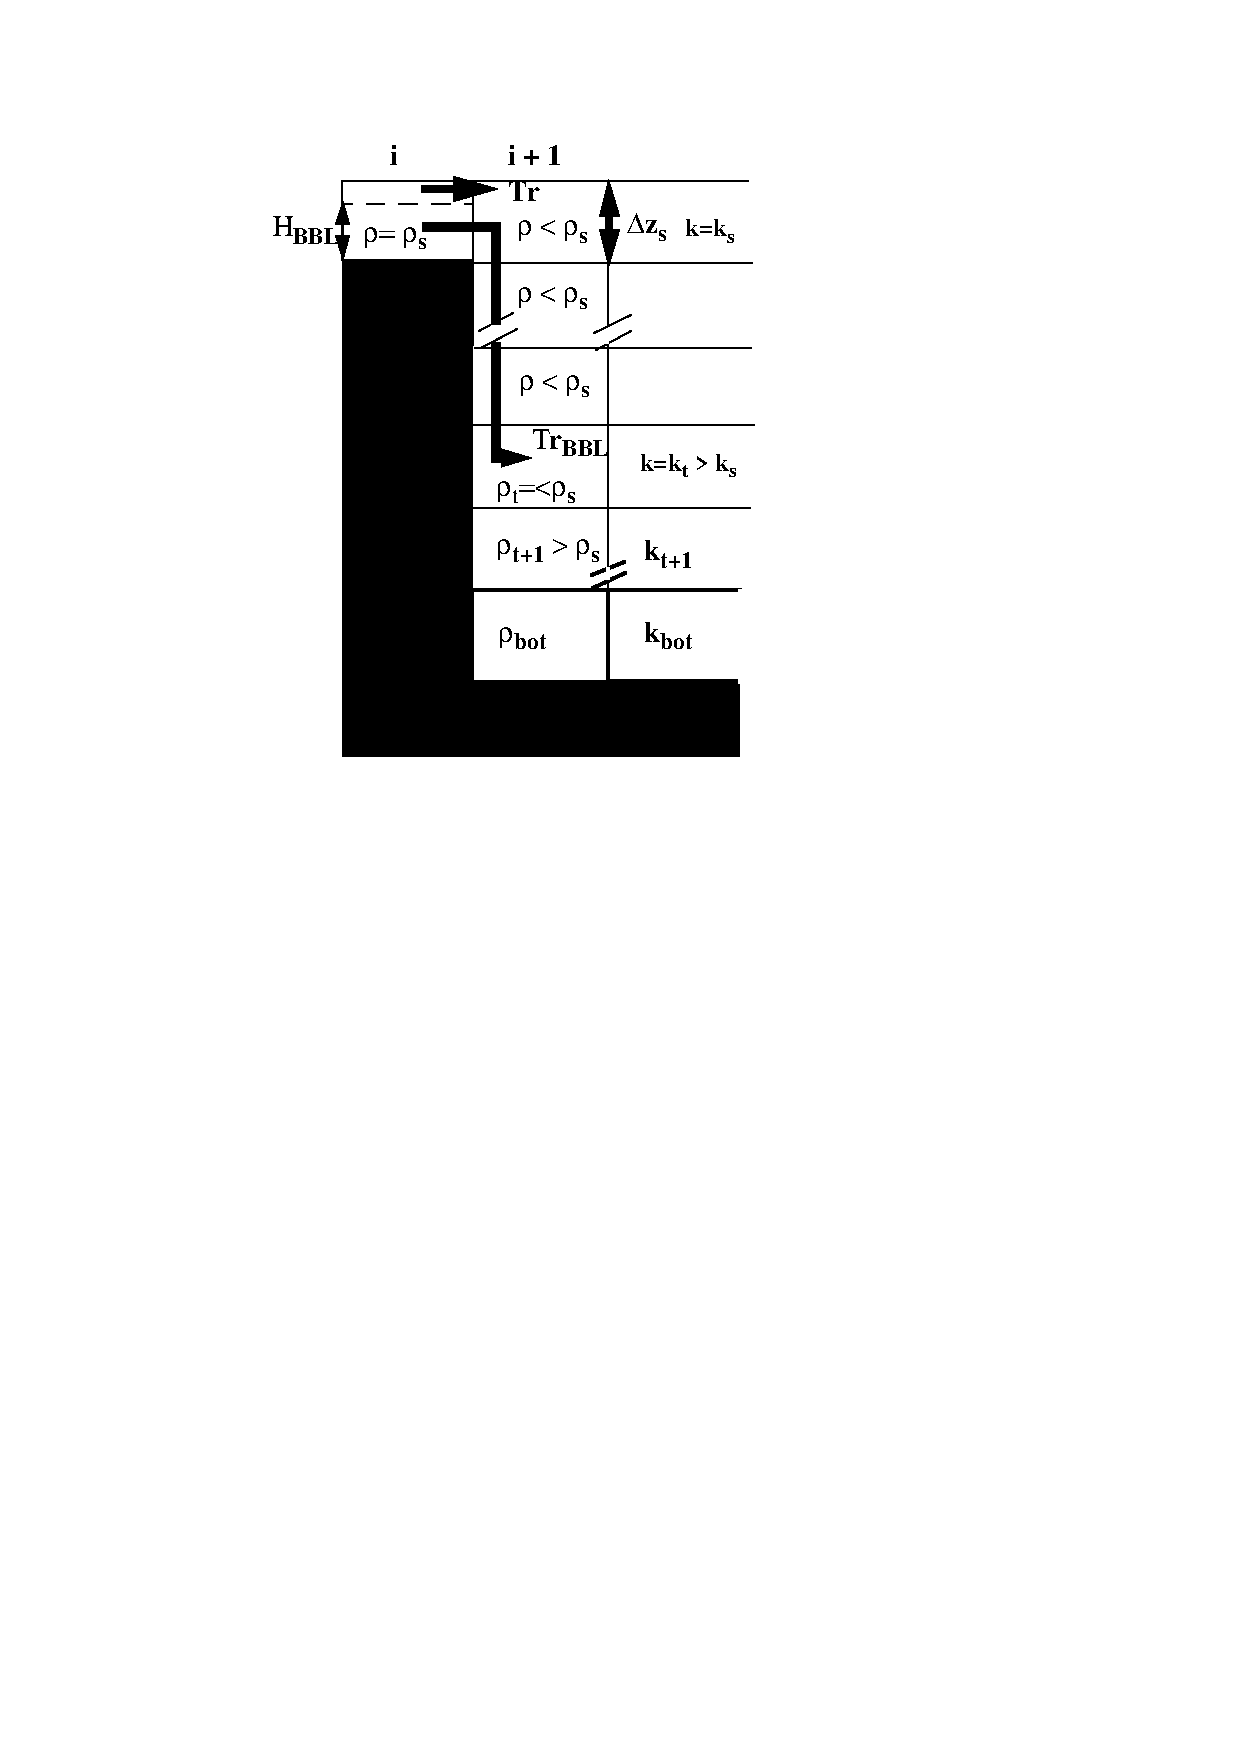
\includegraphics[width=6.cm,angle=0,clip]{bblschem}}}}
\caption{Schematic diagram of the bottom boundary layer advective transport to neutral density level.
Model levels are indicated by k where
k$_s$ and k$_t$ indicate the levels of the source and target cells respectively.
The grid index i refers to either meridional or parallel directions in the curvilinear 
horizontal discretization.
For additional details refer to the text.
}
\label{fig:bbl}
\end{figure}

\subsection{Eddy Viscosity}


The horizontal and vertical eddy viscosity are treated separately.
Horizontal eddy viscosity ${\vec F}_H$ is parameterized 
using a scale-dependent biharmonic formulation
\begin{equation}
\label{eqn:momvisc}
{\vec F}_H =
%- {\vec \nabla_{H}} B_H {\vec\nabla}^3_{H}{\vec v_o}
%- {\vec \nabla_{H}} {\vec B}_H {\vec\nabla_H} \Delta_H {\vec v_o}
- {\vec \nabla_{H}} \cdot \left( B_H {\vec\nabla_H} \Delta_H {\vec v_o} \right)
\end{equation}
where $B_H$ is a coefficient proportional to the fourth power
of the grid spacing.
 
Vertical eddy viscosity ${\vec F}_V$ is parameterized as
\begin{equation}
\label{eqn:vedd}
{\vec F}_V =
{\partial \over {\partial z}}
\left(A_V{\partial \over {\partial z}}{\vec v}_o \right).
\end{equation}
The eddy coefficient $A_V$ is partially relaxed to the value at the previous time step
by use of a time filter to avoid 2$\Delta t$ oscillation.
Using $n$ and $\Lambda_V$ to denote the time increment and relaxation coefficient gives:
\begin{equation}
\label{eqn:vedd2}
{A_V}^n =
\left(1 - \Lambda_V\right){A_V}^{n-1} + \Lambda_V\left(A_{\mathit{VO}}\left(1 + C_{\mathit{RA}}R_i\right)^{-2}
+ A_w + A_b\right).
\end{equation}
The time linear relaxation coefficient $\Lambda_V$ is set to 0.6
in accordance with past experience.
Following Pacanowski and Philander (PP; 1981)\nocite{pacanowski81}
the Richardson number $R_i$ dependent mixing term includes constant coefficients $A_{\mathit{VO}}$ and $C_{\mathit{RA}}$. A small constant background viscosity representing mixing by internal wave breaking is denoted by $A_b$.
The PP scheme in its classical form underestimates turbulent mixing close to the surface. Therefore an additional parameterization for the wind induced stirring $A_w$ is included.  
The near surface wind mixing is proportional to the cube of the local ten meter wind speed $V_{10m}$,
and is reduced in proportion to the fractional sea ice cover $I$.
It decays exponentially with depth and depends on the local static stability $\delta_z \rho$.

\begin{eqnarray}
\label{eqn:awmix}
{A_w(1)}&=&{(1-I) W_T  V_{10m}^3}\\
{A_w(k)}&=&{A_w(k-1) {{\lambda \over{\Delta z}} \over{{\lambda \over{\Delta z}}+ \delta_z \rho}} e^{\Delta z \over{z_0}}  }
\end{eqnarray}
where k=2,3,...,$k_{bot}$ is the vertical level and $\Delta z$ is the level thickness; 
$\lambda$, $z_0$, and $W_T$ are adjustable parameters which were tuned for optimal mixed layer depths.

Tracer diffusion in Eqns~\ref{eqn:tempdiff} and \ref{eqn:saltdiff} 
is represented in two optional ways. The diffusion tensor {\bf K} 
can be chosen either to represent: 
a) standard horizontal/vertical diffusion
\begin{equation}
\label{eqn:khor}
{\bf K} = { D_H \left[ \matrix{1 & 0 & 0 \cr
                     0 & 1 & 0 \cr
                     0 & 0 & \epsilon}\right]}
\end{equation}
with $\epsilon={D_V \over{D_H}}$ ; or
b) isoneutral/dianeutral diffusion

\begin{equation}
\label{eqn:kiso}
{\bf K} = { D_H \left[ \matrix{1 & 0 & S_x \cr
                                0 & 1 & S_y \cr
                   S_x & S_y & \epsilon + S_{\mathit{dif}}^2}\right]}
\end{equation}

with $\epsilon={D_V \over{D_H}}$
and $S_{\mathit{dif}} = (S_x, S_y, 0 )
       = ( {-\delta_x \rho \over{\delta_z \rho}}
       ,   {-\delta_y \rho \over{\delta_z \rho}} 
       ,0 )$.\\ 
The transformation follows \citet{redi82}  with the small slope approximation by 
\citet{gent95}. 
The scheme is numerically implemented following \citet{griffies98b}.
%All the experiments presented in this article utilise 
%isoneutral/dianeutral diffusion.

The effect of tracer mixing by advection with the unresolved mesoscale eddies
is parameterized after Gent et al. (1995).  
 
The vertical eddy diffusivity coefficient $D_V$ is treated similarly to 
Eqn~\ref{eqn:vedd2},
except for the cubic dependence on the shear instability-dependent (Richardson number) term:
\begin{equation}
\label{eqn:hedd}
{D_V}^n =
\left(1 - \Lambda_D\right){D_V}^{n-1} + \Lambda_D\left(D_{\mathit{VO}}\left(1 + C_{RD}R_i\right)^{-3}
+ D_w + D_b\right).
\end{equation}
As with the vertical viscosity,
$D_{\mathit{VO}}$, $C_{RD}$ and the small background term $D_b$ are constant.
The wind-induced term $D_w$ is treated in the same manner as for viscosity.

There are several choices for parameterization of convection currently available in the \mbox{MPI-OM} model.
For details please see \ref{ch:timestepping:octher}

%Convective adjustment follows \citet{bryan69}. 
%Traditionally this technique involved the full mixing of vertically adjacent grid cells 
%in the presence of static instability.
%The \mbox{MPI-OM} formulation is similar but only mixes the upper grid cell with an equivalent thickness
%of the lower grid cell.
%This approach aims to increase the penetrative depth of convection.
%Alternatively \mbox{MPI-OM} allows for the use of a much more physically based parameterization based on the
%penetrative plume convection scheme of \citet{paluszkiewicz97}.
%Plume convection was found to significantly improve the deep water characteristics and
%the simulation of Southern Ocean sea ice in the {HOPE} model \citep{kim2001}.
%However, the penetrative plume convection scheme is computationally quite expensive and is not used
%in the simulations described in this paper.
%The third scheme, and also the one used in this study, is the parameterization of convection
%by greatly enhanced vertical diffusion in the presence of static instability
%(e.g.\ Marotzke, 1991; Klinger at al., 1996). \nocite{marotzke91,klinger96}
%Such an approach avoids the excessive intermediate mixing associated with the traditional adjustment scheme
%by introducing a timescale associated with the choice of (constant) convective-diffusion coefficient.



%%%%%%%%%%%%%%%%%%%%%%%%%%%%%%%%%%%%%%%%%%%%%%%%%%%%%%%%%%%%%%%%%%%%%%%%%%%%%%%
\section{Model Grid}
\label{ch:numeric:grid}




% horizontal discretization
Horizontal discretization of the \mbox{MPI-OM} model is on a staggered Arakawa C-grid \citep{arakawa77}.
The reference grid is shown in figure \ref{fig:numeric:grid:horizontal}.
It consists of prism-shaped finite volumes with the edges aligned with coordinates. 
Vertical discretization is on a so called `z-coordinate' system 
(differentiating from pressure or density coordinate systems).

\subsection{Horizontal discretization}
\label{ch:numeric:grid:horizontal}


\begin{figure}[!!!h]
\centerline{\hbox{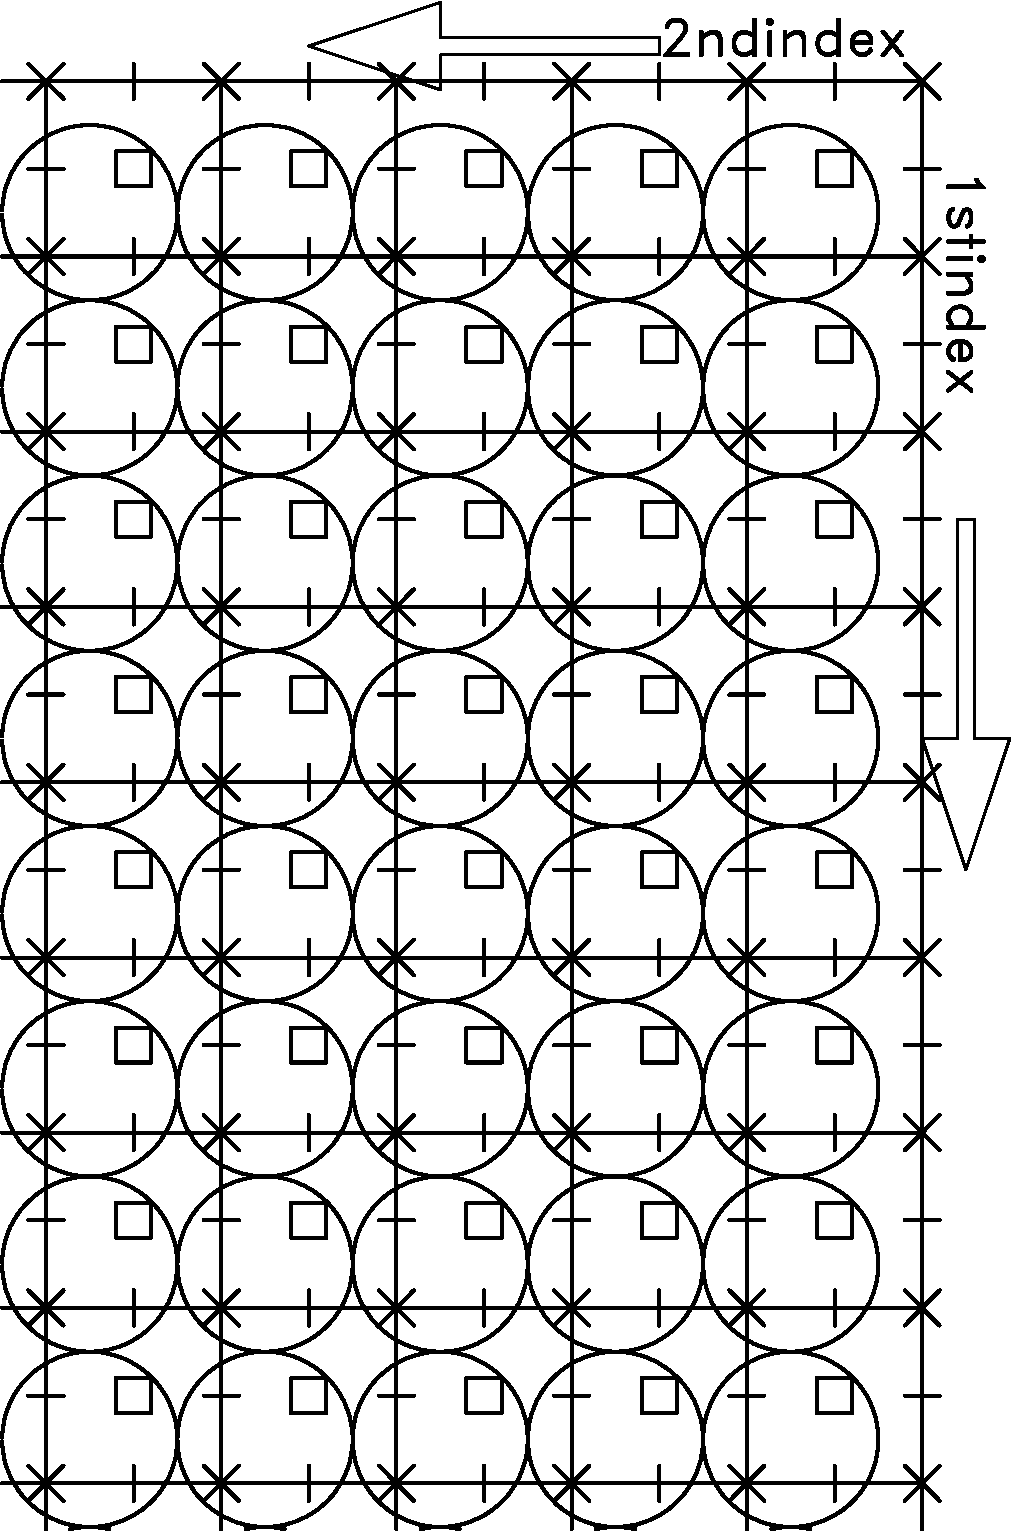
\includegraphics[width=10.0cm,angle=90,clip]{cgricon_new}}}
\mycaption{Layout of the Arakawa C--grid. Boxes denote scalar points, slashes vector points (u in i-direction and v in j-direction) and stars 
the points where the stream function $\psi$ is defined.}
\label{fig:numeric:grid:horizontal}
\end{figure}


Variables defined on vector points are :
\begin{itemize}
\item{horizontal velocities $(u,v)$} 
\item{wind stress $\underline\tau=(\tau^\phi ,\tau^\lambda)$}  
\item{coefficients of vertical viscosity} 
\end{itemize}
Variables defined on scalar points are :
\begin{itemize}
\item{potential temperature $\Theta$} 
\item{salinity $S$} 
\item{density $\rho$} 
\item{pressure $p$} 
\item{vertical velocity $w$}  
\item{coefficients of vertical diffusivity} 
\item{sea surface elevation $\zeta$} 
\item{heat-- and freshwater fluxes across the air sea interface} 
\end{itemize}
Diagnostic stream functions are defined in the $\psi$ points of the grid.

Multiple grid-refinements on an orthogonal grid are possible, i.e.\ MPI-OM calculates a grid using
two vectors, one containing information on longitudes
and one on latitudes. A high resolution in a specified region may cause very ``slim'' grid cells
elsewhere. 

Indexing is done as follows:

West -- East : $\mbox{\tt I} = 1,\ldots,\mbox{\tt IE}$,\\
North -- South : $\mbox{\tt J} = 1,\ldots,\mbox{\tt JE}$,\\
Sea surface -- Bottom : $\mbox{\tt K} = 1,\ldots,\mbox{\tt KE}$

The points with west--east indices 1 and 2
correspond to points with indices {\tt IE-1} and {\tt IE}, respectively,
when periodic boundaries are chosen.


The spherical geometry of the earth is taken into
account by storing all grid distances
$\Delta x(\lambda,\phi)$ and $ \Delta y(\lambda,\phi)$ on arrays, which are then used in the discretization
formulas.

\subsection{Vertical discretization}
\label{ver}

The vertical discretization is the same as used in the {HOPE} model \citep{wolff97},
which includes partial vertical grid cells, i.e.\ at each point in the horizontal grid
the deepest wet cell has a uniform thickness that is adjusted to resolve the discretised bathymetry.
The surface layer thickness is also adjusted to account for the sea surface elevation and 
the sea ice/snow draft where appropriate.

%\vspace{2.0cm}
\unitlength1.0cm
%
\newsavebox{\vecscal}
\savebox{\vecscal}(0,0)[l]{
% plus fuer zeta  2mm
\put(0.4,0.5){\line(1,0){0.2}}
\put(0.5,0.4){\line(0,1){0.2}}
% x fuer vektorpunkte 2mm
\put(1.5,0.5){\circle*{0.2}}
}
%
\newsavebox{\wdot}
\savebox{\wdot}(0,0)[l]{
\put(0.5,0.5){\circle{0.2}}
% abgrenzung i=const
}

\begin{figure}[h]
\begin{picture}(15,9)
% sea surface line at y=9cm
\thinlines
\put(0.,9){\line(1,0){14}}\put(14.3,9.0){\makebox(1,0)[l]{$w_1(z=0)$}}
\put(0.,7){\line(1,0){14}}\put(14.3,7.0){\makebox(1,0)[l]{$w_2, A_{V2}, D_{V2}$}}
\put(0.,3){\line(1,0){14}}\put(14.3,3.0){\makebox(1,0)[l]{$w_k, A_{Vk}, D_{Vk}$}}
\put(0.,0){\line(1,0){14}}\put(14.3,0.0){\makebox(1,0)[l]{$w_{k+1}$}}
\put(14.3,8.0){\makebox(1,0)[l]{$p_1, {\bf v}_1$}}
\put(14.3,5.0){\makebox(1,0)[l]{$p_2, {\bf v}_2$}}
\put(14.3,1.5){\makebox(1,0)[l]{$p_k, {\bf v}_k$}}
%
% scalar vector lines
%
\multiput(6.0,7.75)(2.0,0.0){4}{\usebox{\vecscal}}
\multiput(6.0,4.75)(2.0,0.0){4}{\usebox{\vecscal}}
\multiput(6.0,1.25)(2.0,0.0){4}{\usebox{\vecscal}}
\multiput(6.0,8.75)(2.0,0.0){4}{\usebox{\wdot}}
\multiput(6.0,6.75)(2.0,0.0){4}{\usebox{\wdot}}
\multiput(6.0,2.75)(2.0,0.0){4}{\usebox{\wdot}}
\multiput(6.0,-0.25)(2.0,0.0){4}{\usebox{\wdot}}
%
% topography
%
\thicklines
\put(5.,1.){\line(1,0){4.5}}
\put(9.5,1.){\line(0,1){1.5}}
\put(9.5,2.5){\line(1,0){2}}
\put(11.5,2.5){\line(0,1){1}}
\put(11.5,3.5){\line(1,0){2}}
\put(13.5,3.5){\line(0,1){5.5}}
%
% w-vectors
%
\put(6.5,0.){\vector(0,1){1.0}}
\put(8.5,0.){\vector(0,1){1.0}}
\put(10.5,3.){\vector(0,-1){.5}}
\put(12.5,3.){\vector(0,1){.5}}
%
% distances
%
\put(1.5,8.4){\vector(0,1){0.6}}
\put(1.3,8.0){\makebox(1,0)[l]{$\Delta z_{w1}$}}
\put(1.5,7.6){\vector(0,-1){0.6}}
%
\put(1.3,5.4){\vector(0,1){1.6}}
\put(1.1,5.0){\makebox(1,0)[l]{$\Delta z_{w2}$}}
\put(1.3,4.6){\vector(0,-1){1.6}}
%
\put(1.1,1.9){\vector(0,1){1.1}}
\put(0.9,1.5){\makebox(1,0)[l]{$\Delta z_{wk}$}}
\put(1.1,1.1){\vector(0,-1){1.1}}
%
% distances u-points
%
\put(3.7,8.8){\vector(0,1){0.2}}
\put(3.7,8.5){\makebox(1,0)[l]{$\Delta z_{u1}$}}
\put(3.7,8.2){\vector(0,-1){0.2}}
%
\put(3.5,6.9){\vector(0,1){1.1}}
\put(3.3,6.5){\makebox(1,0)[l]{$\Delta z_{u2}$}}
\put(3.5,6.1){\vector(0,-1){1.1}}
%
\put(3.3,2.8){\vector(0,1){2.2}}
\put(3.1,2.4){\makebox(1,0)[l]{$\Delta z_{uk}$}}
\put(3.3,2.0){\vector(0,-1){0.6}}
%
\put(5.3,0.4){\vector(1,1){0.6}}
\put(1.8,0.5){\makebox(1,0)[l]{Model topography}}
% actual layer thicknesses
\put(7.8,6.0){\vector(0,1){1.0}}
\put(7.6,5.6){\makebox(1,0)[l]{$d_{u2}$}}
\put(7.8,5.2){\vector(0,-1){2.2}}
%
\put(7.8,2.5){\vector(0,1){0.5}}
\put(7.6,2.1){\makebox(1,0)[l]{$d_{uk}$}}
\put(7.8,1.7){\vector(0,-1){0.7}}
%
\put(9.8,6.0){\vector(0,1){1.0}}
\put(9.6,5.6){\makebox(1,0)[l]{$d_{u2}$}}
\put(9.8,5.2){\vector(0,-1){2.7}}
\end{picture}
\caption{\label{fig:numeric:grid:vertical} Vertical structure of model grid }
\end{figure}


The choice of depth values at vector points, and thus the assignment
of layer thicknesses, is free. The vertical velocity component is then
computed  as indicated in fig.\ \ref{fig:numeric:grid:horizontal}.
Model arrays are defined as follows:

\label{depp}
\begin{description}
\item {Array({\sl dimensions})} : description
\item {\tt DZW(KE)} : Vertical distance between two
vertical velocity points (layer thickness). The layer thicknesses
are set in the main program via {\tt DATA DZW / \ldots /} and may be
changed by the user. All other vertical distances are computed from this
array.
\begin{eqnarray*}
  \mbox{\tt DZW(K)} = \Delta z_{wk}\qquad k=1,\ldots,\mbox{\tt KE}
\end{eqnarray*}
%
\item{\tt TIESTW(KE+1)} : Actual depth of $w-$ levels
 ({\tt TIESTW(1)}=0)
\begin{eqnarray*}
 \mbox{\tt TIESTW(K)} = \sum_{l=2}^k \Delta z_{wl-1}\qquad k=2,\ldots,\mbox{\tt KE}
\end{eqnarray*}
\item{\tt TIESTU(KE+1)} : Actual depth of vector/scalar levels
(depend only on $k$)
\begin{eqnarray*}
 \mbox{\tt TIESTU(K)} = {\tt 0.5 * (TIESTW(K+1)-TIESTW(K))}\qquad
 k=1,\ldots,\mbox{\tt KE}
\end{eqnarray*}
\item{\tt DZ(KE)} : Vertical distance between two vector/scalar
 points (for K=1 this is half of the first layer thickness)
\begin{eqnarray*}
 \mbox{\tt DZ(K)} = \Delta z_{uk}\qquad k=1,\ldots,\mbox{\tt KE}
\end{eqnarray*}
%
\end{description}

After a  topography dataset has been supplied on the user specified
grid (at the positions of vector points) MPI-OM recalculates the actual depth of scalar points as
the maximum depth of the four surrounding vector points.
Having done this, local layer thicknesses are computed  taking into account
the adjustment of near bottom vertical velocity points (see fig.\ \ref{fig:numeric:grid:vertical}).

The layer thicknesses are stored on arrays {\tt DDUE, DDUO} and {\tt DDPO}
\begin{description}
\item {${\tt DDU}_{E/O}{\tt (IE,JE,KE)}$} : Layer thicknesses at vector points
\item {${\tt DDPO}{\tt (IE,JE,KE)}$} : Layer thicknesses at scalar points
\end{description}
where E/O indicate the vector points in u and v direction.


\subsection{Curvilinear Coordinate System}
\label{ch:numeric:curvilinear}


\begin{figure}[!tb]%\psdraft
\centerline{\hbox{\includegraphics[height=14.cm,angle=-90,clip]{grob_grid}}}
\caption{Standard \mbox{MPI-OM} orthogonal curvilinear grid for global climate study applications at MPIfM.}
\label{fig:numeric:antagrid}
\end{figure}

% curvilinear coord system
The \mbox{MPI-OM} model uses a bipolar orthogonal spherical coordinate system.
If the poles are antipodes (diametrically opposed) then the coordinate system
is reduced to a rotated spherical grid.
Otherwise, orthogonal meridians and parallels are constructed
according to the choice of zonal and meridional resolution and are used to define the spatial mesh.
Although it may be desirable to maintain `quadrature' of the grid
(i.e.\ within each grid cell the local zonal and meridional grid distances are equal),
it is by no means a necessary condition.
Two advantages can be achieved by assignment of a radius to the poles.
Firstly, land points can be removed from the computational matrix.
Secondly, by choosing non-equal pole radii horizontal resolution can be
concentrated about the pole of smaller radius for regional studies.
Implementation of the curvilinear grid is relatively straightforward
but does require 
some additional computational expense.
In terms of memory many additional arrays must be added for storage of all terms
related to horizontal metrics between both scalar and vector neighboring pairs.
The processing time is therefore extended for all operations including horizontal metrics
that could otherwise be factored on a regular grid.
This condition is omnipresent throughout the model code with the exception of purely vertical
operations such as convection.

The standard MPIfM horizontal ocean grid used for climate studies has traditionally been at a spatial resolution
approximating spectral truncation T42 with additional equatorial meridional grid refinement
(e.g.\ HOPE, Legutke and Voss, 1999; OPYC, Roeckner at al., 1999). \nocite{legutke99,roeckner99}
With the 2005 IPCC experiments this has changed to the GROB15 grid with a formal
resolution of 1.5~\degs. In this setup,
one pole is located over Greenland and the other over Antarctica.
The horizontal resolution gradually varies between 10 km in the Arctic
and about 170 km in the Tropics. This arrangement gives highest resolution in the 
main sinking regions associated with the thermohaline circulation (THC).
It has 40 vertical levels with level
thickness increasing with depth. Eight layers are within the upper 90 m
and 20 are within the upper 600m. Also common is the GR30 setup with a formal
resolution of 3.0~\degs.
The models bathymetry was created by interpolation of the
ETOPO-5 dataset (Data Announcement 88-MGG-02, Digital relief of the
Surface of the Earth. NOAA, National Geophysical Data Center, Boulder,
Colorado, 1988) to the model grid.
The spectral truncation T42 grid and other grid versions, 
used for more regionally focused studies, are shown in \citet{Marsland:2003}.


%===========================================================================

\section{Bulk Formulae}
\label{sec:bulkformule}
Simulation with the ocean model requires the specification of heat,
fresh water and momentum fluxes at the air/sea interface. 
Introducing $Q_{\mathit{srf}}$ to denote either $Q_{w}$ or $Q_{i}$ in Eqn~\ref{eqn:icethermo}
the surface heat balance is given by
\begin{equation}
\label{eqn:icethermo1}
Q_{\mathit{srf}} = Q_{\mathit{srf}}^{\mathit{se}} + Q_{\mathit{srf}}^{\mathit{la}}
+                  Q_{\mathit{srf}}^{\mathit{lw}} + Q_{\mathit{srf}}^{\mathit{sw}}
\end{equation}
where $Q_{\mathit{srf}}^{\mathit{se}}$, $Q_{\mathit{srf}}^{\mathit{la}}$,
$Q_{\mathit{srf}}^{\mathit{lw}}$ and $Q_{\mathit{srf}}^{\mathit{sw}}$
are parameterizations of the sensible, latent, long-wave and short-wave heat fluxes, respectively.

Following \citet{oberhuber93} the turbulent fluxes are parameterized as
\begin{eqnarray}
%
% sensible
%
\label{se}  Q_{\mathit{srf}}^{\mathit{se}}             &=&
\rho_{a}c_{a}C_{H}V_{\mathit{10m}}(T_{a} - T_{\mathit{srf}})            \\
%
% latent
%
\label{la} Q_{\mathit{srf}}^{\mathit{la}}              &=&
\rho_{a}L_{\mathit{srf}}C_{L}V_{\mathit{10m}}(q_a - q_{\mathit{srf}})
\end{eqnarray}
Constants $\rho_a$, $c_a$ and $L_{\mathit{srf}}$ denote the air density,
the air specific heat capacity and the latent heat of vaporization or sublimation as appropriate.
The 10~m wind speed $V_{\mathit{10m}}$ and 2~m air temperature $T_{a}$ are taken as prescribed forcing.
Variable coefficients of sensible $C_H$ and latent $C_L$ heat transfer 
are formulated according to \citet{large82}.
The surface temperature $T_{\mathit{srf}}$ represents either the ocean model upper layer temperature
or the sea ice/snow layer skin temperature as in Eqn~\ref{cond1}.
The specific humidity $q$ is a function of water vapor pressure $e$ (units of Pascal)
and air pressure $p$ (currently approximated by a constant 1000 hPa in MPI-OM-1).
\begin{equation}
q = (0.623e)/(p-0.378e)
\end{equation}
At the 2~m level ($q_a$) the water vapor pressure is a function of dew point temperature,
while at the surface ($q_{\mathit{srf}}$) the saturation vapor pressure 
is a function of the water or ice/snow surface temperature.
In both cases the vapor pressures ($e$) are calculated according to the formulae of \citet{buck81}.
 
The radiant fluxes are parameterized as 
\begin{eqnarray}
%
% longwave
%
\label{lw} Q_{\mathit{srf}}^{\mathit{lw}}              &=&
\varepsilon \sigma T_{a}^{4} (.39-.05 \sqrt{e/100})(1-{\chi}n^2)
+ 4\varepsilon \sigma T_a^3(T_{\mathit{srf}} - T_a)         \\
%
% shortwave
%
\label{sw}  Q_{\mathit{srf}}^{\mathit{sw}}             &=&
 (1-\alpha_{\mathit{srf}})Q^{\mathit{incsw}}
%
\end{eqnarray}
The parameterization of net longwave radiation is based on that of \citet{berliand52},
with the fractional cloud cover $n$ taken as prescribed forcing.
The surface thermal emissivity and Stefan-Boltzmann constant are denoted by
$\varepsilon$ and $\sigma$ respectively.
The saturation vapor pressures $e$ depend on water or sea ice/snow conditions and are also calculated
according to the formulae of \citet{buck81}.
The cloudiness factor $\chi$ is a modified form of that proposed by \citet{budyko74} and is a function
of latitude $\phi$.
\begin{equation}
\chi = 0.5 + 0.4 ( \min (|\phi|,60^{\circ}) )/90^{\circ}
\end{equation}
The incident shortwave radiation $Q^{\mathit{incsw}}$ is 
provided as part of the forcing data and implicitly modified 
by cloud cover in the ERA model.
The surface reflectivity $\alpha_{\mathit{srf}}$ in Eqn~\ref{sw}
is either that appropriate for open water or
takes one of four possible values determined by both the
absence or presence of snow
and by whether the surface temperature
of the sea ice or snow is below 0$^{\circ}$C (freezing)
or equal to 0$^{\circ}$C (melting).
\begin{equation}
\label{eqn:albedo}
\alpha_{\mathit{srf}} = \left\{ \begin{array}{cc}
\alpha_{\mathit{w}}  & \mbox{open water} \\
\alpha_{\mathit{im}} & \mbox{sea ice surface and melting} \\
\alpha_{\mathit{if}} & \mbox{sea ice surface and freezing} \\
\alpha_{\mathit{sm}} & \mbox{snow surface and melting} \\
\alpha_{\mathit{sf}} & \mbox{snow surface and freezing}
                                \end{array}
                         \right.
\end{equation}
Over open water $Q_{\mathit{w}}^{\mathit{sw}}$ is allowed to penetrate
beyond the upper model layer with an exponential decay profile.
% In the experiments considered in Section~\ref{ch:numeric:curvilinear}
% approximately 15\% of $Q_{\mathit{w}}^{\mathit{sw}}$
% is redistributed to deeper model levels  (mostly to the second level).

%para SFWF
The surface freshwater forcing effect on sea level displacement
is given by
\begin{equation}
\label{eqn:sfwf1}
Q_{\zeta} = P - E + R + G
\end{equation}
where $P$, $E$, $R$ and $G$ are fluxes of freshwater in units of \mbox{m s$^{-1}$} due to
precipitation, evaporation, river runoff and glacial meltwater, respectively.
For the ocean only simulations considered here 
$P$ is taken as prescribed forcing,
$R$ is taken from
the observed mean monthly discharge of the world's 50 largest rivers \citep{duemenil93},
and $G$ is neglected.
Finally, $E$ is calculated from the latent heat flux (Eqn~\ref{la}) as
\begin{equation}
\label{eqn:evap}
E = 
Q_{\mathit{srf}}^{\mathit{la}}/(L_{\mathit{srf}}\rho_{w})
%\left\{ \begin{array}{lcll}
%V_{\mathit{10m}} \left(
%    (1-I)C_{L\mathit{o}}{\rho_a \over \rho_o} (q_a - q_{\mathit{o}}) 
%\right.&+&\left.   I C_{L\mathit{i}}{\rho_a \over \rho_i} (q_a - q_{\mathit{i}}) \right)
%& \mbox{for ice surface} \\
%V_{\mathit{10m}} \left(
%    (1-I)C_{L\mathit{o}}{\rho_a \over \rho_o} (q_a - q_{\mathit{o}})
%\right.&+&\left.   I C_{L\mathit{s}}{\rho_a \over \rho_s} (q_a - q_{\mathit{s}}) \right)
%& \mbox{for snow surface}
%\end{array}\right.
\end{equation}
where 
$\rho_{w}$ is the density of sea water and $L_{\mathit{srf}}$
is once again the latent heat of vaporization or sublimation as appropriate
for water or ice/snow surfaces respectively.
%$q_{\mathit{o}}$ ($C_{L\mathit{o}}$), 
%$q_{\mathit{i}}$ ($C_{L\mathit{i}}$) and $q_{\mathit{s}}$ ($C_{L\mathit{s}}$)
%denote the specific humidities (exchange coefficients of latent heat) 
%over open water, ice and snow respectively.
The corresponding change in surface model layer salinity $\Delta S_1$ is given by
\begin{equation}
\label{eqn:numeric:sfwf2}
\Delta S_1 = \left( {\Delta z_1 + Q_{\zeta} \over {\Delta z_1}} \right) S_1 + ( S_1 - S_{\mathit{obs}})/S_R
\end{equation}
where 
$S_R$ is a time-linear restoring coefficient (units s$^{-1}$),
and $S_{\mathit{obs}}$ is a prescribed observed (monthly or annual) surface salinity (see also equation~\ref{eqn:numeric:relaxation}).
%The Salinity restoring for the experiments considered in Section~\ref{ch:numeric:curvilinear} 
%has a timescale (inverse) of 39~days which is quite strong.
The salinity restoring helps to correct for an 
unbalanced globally integrated surface freshwater flux,
along with errors in the poorly known forcing fields ($P$, $R$, and $G$).
The restoring has the positive effect of reducing long term model drift.
However, it does damp model variability.
A more thorough discussion of the effects of surface relaxation is given by \citet{killworth2000}.
The timescale of the restoring is set in the namelist (see table \ref{tb:using:namelist}), restoring to a monthly climatology is an 
option which requires a CPP switch (Section~\ref{ch:using:compiling:conditional}).

%para surface wind stress
Momentum forcing by atmospheric wind stress over sea ice is applied directly in Eqn.~\ref{eqn:icemomentum}.
For the ocean surface layer velocity $\vec{v_1}$,
the wind stress over open water and the ocean-ice stress otherwise 
result in a change of
\begin{equation}
\label{eqn:ocstress}
{\partial \vec{v_1} \over {\partial t}} = 
{1-I \over {\rho_w \Delta z_1}} \vec{\tau_a}
+{I \over {\rho_w \Delta z_1}} \vec{\tau_i}
%         TAUWATU(I,J)=CW*RHOICWA*SPEEDU(I,J)*(SICUO(I,J)-UKO(I,J,1))
%      UOO(I,J,1)=UOO(I,J,1)+DTDECT*AMSUO(I,J,1)*(TXO(I,J)*UR
%     X  +(1.-UR)*AMSUO(I,J,1)*TAUWATU(I,J))
\end{equation}
where the ice to ocean stress $\vec{\tau_i} = -\vec{\tau_o}$ from Eqn~\ref{eqn:icestress}.

%===========================================================================
\section{OMIP Atmospheric Forcing}
\label{sec:numeric:omip}

The OMIP forcing is a climatological forcing dataset with daily temporal resolution
and atmospheric synoptic scale variability. It provides the 
heat, freshwater and momentum fluxes at the air/sea interface required by the \mbox{MPI-OM} model
The forcing data is taken from the German Ocean Model Intercomparison Project (OMIP)
climatology, and hereafter is called the OMIP-forcing.
OMIP was a collaboration between MPIfM,
the German Climate Computing Center (DKRZ)
and the Alfred Wegener Institute for Polar and Marine Research.
The OMIP project 
\footnote{www.mpimet.mpg.de/Depts/Klima/natcli/omip/omip\_report.html}
compared the mean state of the global circulation of {HOPE}
with that of the Modular Ocean Model (MOM2; Pacanowski, 1995). \nocite{pacanowski95}
Considerable emphasis was also placed on the generation of a surface heat and
freshwater flux climatology.
The OMIP-forcing was derived from the ECMWF Re-Analysis (ERA; Gibson et al., 1997)\nocite{gibson97} 
15 year dataset and is documented by \citet{roeske01}.

Three criteria were used for the design of the OMIP-forcing:
that the forcing be global;
that the forcing resolves timescales associated with weather systems;
and that the horizontal resolution of the forcing be somewhat finer than that
commonly used in OGCMs.
The forcing was constructed by Gaussian filtering of the ERA data
to produce a low-frequency and a high-frequency component.
The low-frequency components from all years were averaged to create a single mean year.
Then the high-frequency component of a single year 
was superimposed onto the mean year to maintain
quasi-realistic synoptic scale space-time variability.
The criterion for choosing a particular year for the high-frequency component
was to maximize the variance of the OMIP-forcing relative to the
variance of the original ERA data.
For dynamical consistency it was considered desirable to choose
only one high-frequency year for all forcing products (winds, temperatures etc).
As different products have maximum variance in different years,
the maximization of variance was arbitrarily limited to zonal wind stress.
This resulted in the choice of the year 1982,
with preservation of 78\% of the original ERA
variability relative to monthly means.

%===========================================================================

\section{NCEP/NCAR Atmospheric Forcing}
\label{sec:numeric:ncep}
The NCEP/NCAR reanalysis is a dataset with daily
temporal resolution and atmospheric synoptic scale variability
\citep{kalnay96}. Daily 2 m air and dew-point temperatures,
precipitation, cloud cover, downward shortwave radiation, 10 m wind
speed and surface wind stress are available for the full period
that is covered by the NCEP/NCAR reanalysis (1948-today). Dew point
temperature $T_{Dew}$ is derived from specific humidity $q$ and air
pressure $p$ according to \cite{oberhuber88}.

\begin{eqnarray}
\label{tdew}
e & = & q * p / (0.378 * q + 0.623)\\
\alpha & = & 1 / 7.5 * (log_{10} * e/611)\\
T_{Dew} & = & (273.16 - (35.86 * \alpha ))/(1-\alpha)
\end{eqnarray}

On global average NCEP/NCAR downward short wave radiation is
appr.~10\% higher than ECMWF reanalysis data and 20\% higher
than ERBE estimates. To correct for this systematic offset in the
NCEP/NCAR downward shortwave radiation a global scaling factor of 0.89
can be applied by using an CPP switch (Section~\ref{ch:using:compiling:conditional}). 



% work areas are denoted by #####
%
%
%new intro chapter starting 31/05/01

%$Source: /server/cvs/mpiom1/mpi-om/doc/tecdoc_mpiom/Attic/c5.tex,v $\\
%$Revision: 1.1.2.1.4.2.2.2.2.3.2.1 $\\
%$Date: 2006/03/07 14:50:43 $\\
%$Name: mpiom_1_2_0 $\\


%\pagenumbering{arabic}
\thispagestyle{empty}
 
\chapter[Time Stepping]
{\Large{\bf Time Stepping}\label{ch:timestepping}}


\section{Time stepping method}
\label{ch:timestepping:method}


The motions associated with the vertically integrated velocity field (barotropic
part) are solved implicitly which  damps the external
gravity wave mode and thus allows the use of  a longer time-step in the integrations.
Time stepping in MPI-OM is based on the idea of operator splitting, which
is also called {\sl time splitting} or {\sl method of fractional steps},
as described by e.g.\ \citet{press88}. 
The method is illustrated with the following example (taken from \citet{press88}).

Suppose you have an initial value equation of the form
\begin{eqnarray}
{{\partial u}\over{\partial t}} = \mbox{\op L}u
\end{eqnarray}
where {\op L} is some operator. While {\op L} is not necessarily linear, suppose that it can
at least be written as a linear sum of $m$ pieces, which act additively on $u$,
\begin{eqnarray}
\mbox{\op L}u=\mbox{\op L}_1u+\mbox{\op L}_2u + \cdots \mbox{\op L}_m u
\end{eqnarray}
Finally, suppose that for each of the pieces, you already know a differencing scheme
for updating the variable $u$ from time-step $n$ to time-step $n+1$, valid if
that piece of the operator were the only one on the right-hand side. We will write
these updating symbolically as
\begin{eqnarray}
u^{n+1} & = & \mbox{\op U}_1(u^n,\Delta t)\nonumber \\
u^{n+1} & = & \mbox{\op U}_2(u^n,\Delta t)\nonumber \\
        & \cdots & \\
u^{n+1} & = & \mbox{\op U}_m(u^n,\Delta t)\nonumber
\end{eqnarray}
Now, one form of operator splitting would be to get from $n$ to $n+1$ by the
following sequence of updating:
\begin{eqnarray}
u^{n+(1/m)} & = & \mbox{\op U}_1(u^n,\Delta t) \nonumber \\
u^{n+(2/m)} & = & \mbox{\op U}_2(u^{n+(1/m)},\Delta t) \nonumber \\
            & \cdots & \\
u^{n+1} & = & \mbox{\op U}_m(u^{n+(m-1)/m},\Delta t) \nonumber
\end{eqnarray}

This operator splitting is used in {\sl MPI-OM}.

%%%%%%%%%%%%%%%%%%%%%%%%%%%%%%%%%%%%%%%%%%%%%%%%%%%%%%%%%%%%%%%%%%%%%%%%%%%%%%%%%
% Klar wie Klosbruehe
\section{Timestepping in the Model}
\label{ch:timestepping:model}

The timestepping proceeds by the method of operator splitting or fractional steps
as described in Section~\ref{ch:timestepping:method}. 
That is, prognostic variables are updated
successively in several subroutines.
Prescribed forcing is read in at the start of each time-step after which the 
sea ice dynamics equations are solved by means of 
%successive over-relaxation with Chebychev acceleration.
functional iteration with under relaxation.
Then the sea ice thermodynamics are implemented.
The ocean momentum equation  is first solved partially for the friction terms and 
then the advection terms.
This results in a partially updated momentum equation which is 
decomposed into baroclinic and barotropic subsystems.
These are solved separately as described below.
As in HOPE \citep{wolff97} the prognostic equation for the free surface is solved
implicitly, which allows for the model's barotropic time-step
to equal the baroclinic time-step.

All subroutine called during one time step are listed in table \ref{tb:timestepping:sbr}
and are described in the following.
All symbols are explained in section \ref{sec:appendix:los} ``list of variables''.


\begin{table}[ht]
\begin{footnotesize}
        \begin{tabular}[t]{l|p{8cm}|l}
        \hline
          SBR name &
          Action &
          Ref. \\
        \hline\hline
         \texttt{octher.f90} &	   
           -boundary forcing on salt and temperature
	   
           -baroclinic pressure
	   
           -convective adjustment
	   
           -vertical eddy viscosity and diffusivity coefficients &
          \ref{ch:timestepping:octher} \\	  
         \texttt{-ocice.f90} &
	   Sea ice model as described by \citet{hibler79}&
          ch. \ref{ch:ice} \\		  
         \texttt{--growth.f90} &
	   Update of ice thickness, compactness, snow depth, upper ocean
           temperature and salinity due to atmospheric heat and freshwater fluxes.
          \\	
         \texttt{ocwind.f90} &
	   Update ocean velocities with the surface stress (wind forcing).&
          \ref{ch:timestepping:ocwind} \\
         \texttt{octide.f90} &
	   Include forcing from tides (optional).&
          \\
         \texttt{ocmodmom.f90} &
	   Decomposition into barotropic and baroclinic field.&
          \ref{ch:timestepping:ocmodmom} \\
%         \texttt{ocbarp.f90} &
%	   &
%          \\
         \texttt{occlit.f90} &
	   Solution of the baroclinic system.&
          \ref{ch:timestepping:occlit} \\
         \texttt{bartim.f90} &
	   Calculate sea level hight for the barotropic subsystem with gauss elimination and back-substitution (default).&
          \ref{ch:timestepping:bartim}\\
         \texttt{troneu.f90} &
	   Calculate sea level hight for the barotropic subsystem with iterative solver (SOR, optional).&
          \ref{ch:timestepping:troneu}\\
         \texttt{ocvtro.f90} &
	   Calculate new barotropic velocities.&
          \ref{ch:timestepping:ocvtro}\\
         \texttt{ocvtot.f90} &
	   Calculate new total velocities $u, v$ and $w$.&
          \ref{ch:timestepping:ocvtot}\\	  
         \texttt{ocuad.f90} &
	   Advection of momentum analogous to \texttt{ocadpo.f90} in u direction.&
          \ref{ch:timestepping:ocuad}\\	  
         \texttt{ocvad.f90} &
	   Advection of momentum analogous to \texttt{ocadpo.f90} in v direction.&
          \\		  
         \texttt{slopetrans.f90} &
	   Calculate bottom bondary layer (BBL) transport for tracer advection (optional).&
          \ref{ch:timestepping:slopetrans}\\		  
         \texttt{ocadpo.f90} &
	   Computes advection with a second order total variation diminishing (TVD) scheme 
	   \citep{Sweby:1984}. Called for temperature and salinity (optional).&
          \ref{ch:timestepping:ocadpo}\\		  
         \texttt{ocadfs.f90} &
	   Compute advection with predictor-corrector scheme
           or the quick-scheme as proposed by \citet{Farrow:1995} (optional).&
          \ref{ch:timestepping:ocadfs}\\		  
         \texttt{ocjitr.f90} &
	   Parameterize sub grid-scale eddy-induced tracer transport
           following \citet{Gent:1995} (optional).&
          \ref{ch:timestepping:ocjitr}\\	  
         \texttt{octdiff\_base.f90} &
	   Compute tracer-independent matrices for horizontal, isopycnal diffusion.&
          \ref{ch:timestepping:octdiff-base}\\		  
         \texttt{octdiff\_trf.f90} &
	   Calculate vertical diffusion and 
	   harmonic and biharmonic horizontal diffusion 
	   (with matrices calculated in \texttt{octdiff\_base.f90})
	   for temperature and salinity.&
          \ref{ch:timestepping:octdiff-trf}\\	  	  
         \texttt{relax\_ts.f90} &
	   3-D restoring of temperature and salinity to initial conditions.&
          \ref{ch:timestepping:relax-ts}\\	
%         \texttt{octimf.f90} &
%	   Update u and v velocities with ... ???? &
%          \\		  
         \texttt{ocschep.f90} &
	   Harmonic horizontal diffusion of momentum. &
          \ref{ch:timestepping:ocschep}\\		  
         \texttt{ocvisc.f90} &
	   Vertical diffusion of momentum, 
	   bottom friction, biharmonic horizontal momentum diffusion &
%	   and shear dependent diffusion&
          \ref{ch:timestepping:ocvisc}\\			  
        \end{tabular}
\end{footnotesize}
\caption{List of subroutine calls during one time-step.}
\label{tb:timestepping:sbr}
\end{table}


\subsection{octher.f90}
\label{ch:timestepping:octher}
\subsubsection{boundary forcing}

TO DO: The source has to be cleaned up. Encapsulate different parameterizations. 
CPP flag "NURMISCH" is identical to "CDVOCON == 0".  "NURDIFF" has to be default.

In ice free or non--compact ice covered areas the salinity is changed according to
\begin{eqnarray}
S^{n+1/m}\bigg\vert_{k=1}& = &S^n\bigg\vert_{k=1} + \Delta t\lambda_{S}\left(
                 S_{Levitus} - S^n\bigg\vert_{k=1}\right)\cdot (1-A)
\end{eqnarray}
where $A$ is the sea ice compactness. The salinity is further modified
in the sea ice model due to freezing or melting processes.
In addition, the sea surface temperature can relaxed to a SST climatology \citep{Levitus:1998}
\begin{eqnarray}
\Theta^{n+1/m}=\Theta_1^n + \Delta t \: \lambda_T\cdot(\Theta_{Levitus}-\Theta^n\bigg\vert_{k=1})
\end{eqnarray}
Default for the time constants is $\lambda_{S} = 3.*10^{-7}$ and $\lambda_{T} = 0.$ 
$\lambda_{S}$ and $\lambda_{T}$ can be modified in the namelist (\ref{tb:using:namelist}).
Both are weighted with the actual thickness of the first layer with respect to a thickness of 20~m
($\lambda = \lambda_{namelist}*20~m/DZW_{(1)}$).
Salinity and temperature restoring does only work if MPI-OM is not coupled to ECHAM. 
 
\clearpage
 
Discharge from rivers is affecting salinity and sea surface elevation. 
\begin{eqnarray}
S^{n+1/m}\bigg\vert_{k=1}& = &S^n\bigg\vert_{k=1} + {{\Delta z_{w}}\over{\Delta z_{1} + \Delta R_{input}}}\\
ZO^{n+1/m}& = &ZO + \Delta R_{input}\\
\end{eqnarray}
Local river input is calculated from discharge data for the given position (see section \ref{sec:using:input}):
\begin{eqnarray}
\Delta R_{input}& = &{{discharge*\Delta t}\over{\Delta x*\Delta y}}
\end{eqnarray}
 
%DRIV=GIRIV(I,J)*DT/(DLXP(I,J)*DLYP(I,J))
%     SAO(I,J,1)=SAO(I,J,1)*ZZZDZ/(ZZZDZ+DRIV)
%      ZO(I,J)=ZO(I,J)+DRIV


\subsubsection{baroclinic pressure and stability}


Hydrostatic pressure and stratification is computed.
Potential temperatures $\Theta$ are converted to in--situ temperatures $T$ (subroutine \texttt{adisitj.f90})
by solving the \citet{Gill:1982} formula with a Newton's method.
The density is computed in subroutine \texttt{rho1j.f90} with the \citet{unesco83} formula.

\begin{eqnarray}
p_1 &=& g\Delta z_{w1}\: \rho\left(S_1^{n+2/m}, T_1^{n+2/m}, p_{1(ref)}\right)\\
p_k &=& p_{k-1} + g\Delta z_{wk}\: \rho\left(S_k^{n+2/m}, T_k^{n+2/m}, p_{k(ref)}\right)\\
{{\partial\rho_k}\over{\partial z}} &=& {1\over\Delta z_{uk}} (\rho_{k-1}-\rho_k)^{n+2/m}
\end{eqnarray}
where the density $\rho$ is calculated using a reference pressure
\begin{eqnarray}
p_{(ref)k}= g\rho_0 h_k
\end{eqnarray}
where $h_k$ is the  depth of layer $k$.

There are several choices for parameterization of convection currently available in the \mbox{MPI-OM} model.
\begin{itemize}
\item
Default in cases of unstable stratification is a combination of vertical diffusion and mixing.
Other mechanisms are activated with compile flags (table \ref{tb:using:cpp-flags-physical}). 
\item
Compile flag "NURDIFF" disables the default mixing.
\item
Compile flag "UMKLAP" activates the convective adjustment. 
Convective adjustment follows \citet{bryan69}.
Traditionally this technique involved the full mixing of vertically adjacent grid cells 
in the presence of static instability.
The \mbox{MPI-OM} formulation is similar but only mixes the upper grid cell with an equivalent thickness
of the lower grid cell.
This approach aims to increase the penetrative depth of convection.
It is done with only one sweep through the water column per timestep, i.e.
for $\rho_z > 0$
\begin{eqnarray}
\Theta_k^{n+3/m} = {{\displaystyle \Delta z_{wk-1}\Theta_{k-1}^{n+2/m}+\Delta z_{wk}\Theta_{k}^{n+2/m}}\over
               {\displaystyle \Delta z_{wk-1}+\Delta z_{wk}}}\\
S_k^{n+3/m} = {{\displaystyle \Delta z_{wk-1}S_{k-1}^{n+2/m}+\Delta z_{wk}S_{k}^{n+2/m}}\over
               {\displaystyle \Delta z_{wk-1}+\Delta z_{wk}}}
\end{eqnarray}
for stable stratification $\rho_z < 0$ (or {\tt ICONVA = 0})
\begin{eqnarray}
\Theta_k^{n+3/m} =\Theta_{k}^{n+2/m}\\
S_k^{n+3/m} =S_{k}^{n+2/m}
\end{eqnarray}
If convective adjustment was active the stratification array is adjusted.

\item
Compile flag "PLUME" activates the so-called "PLUME" convection scheme (subroutine \texttt{nlopps.f90}). 
It is based on an original routine by E. Skyllingstad and T. Paluszkiewicz.
It is a much more physically based parameterization based on the
penetrative plume convection scheme of \citet{paluszkiewicz97}.
Plume convection was found to significantly improve the deep water characteristics and
the simulation of Southern Ocean sea ice in the {HOPE} model \citep{kim2001}.
However, the penetrative plume convection scheme is computationally quite expensive.
%For the parameter setting {\tt IEDDY = 1}

\item
If the compile flag  "NURMISCH" is set, only the  Richardson number depending coefficients are used for the diffusion.
Richardson number depending  coefficients for eddy viscosity and eddy diffusivity 
are computed every timestep \citep{pacanowski81}.
%(see e.g.\ Pacanowski and Philander, 1981, Monin and Yaglom, 1971, Jones, 1973).
Additionally, a mixed layer turbulence contribution is included.

\begin{eqnarray}\label{av1}
A_V^{\bf n+1} &=& \lambda_V A_V^n + (1-\lambda_V)\left[ {A_{V0}\over{1+(C_{RA} Ri)^2}}
\right] + A_B+ \delta_{\Delta T} W_T \\ \label{dv1}
D_V^{\bf n+1} &=& \lambda_V D_V^n + (1-\lambda_V)\left[ {D_{V0}\over{1+(C_{RD} Ri)^2}}
\right] + \delta_{\Delta T} W_T
\end{eqnarray}

where $0 \leq \lambda \leq 1$, $A_{V0}$ and $D_{V0}$ are constant values,
$A_B$ is the background mixing (set to $10^{-6}\mbox{ m}^2/\mbox{s}^{-1}$),
 $W_T$ is a value for
a wind induced mixed layer turbulence (increased turbulent
viscosity and diffusivity), $\delta_{\Delta T}$ is a
switch which is 1 for a vertical temperature difference to the sea surface temperature smaller than a preset $\Delta T$
and 0 elsewhere, and $Ri$ is the local Richardson number
\begin{eqnarray}
Ri = - {{g\partial\rho/ \partial z}\over{(\partial  u/ \partial z)^2+(\partial v/ \partial z)^2}}
\end{eqnarray}
Eqs.\ (\ref{av1}) and (\ref{dv1}) are slightly modified with respect to
the original formulations by \citet{pacanowski81}.

% For {\tt IEDDY = 0}
% all eddy coefficients are set constant in time and space.
\item
If the compile flag  "NURMISCH" is not set,
in cases of unstable stratification the coefficient is replaced by the mixing term "CDVOCON" which is set in the 
namelist (table \ref{tb:using:namelist}), if "CDVOCON" is larger that the Richardson coefficient.
This leads to a greatly enhanced vertical diffusion in the presence of static instability
(e.g.\ Marotzke, 1991; Klinger at al., 1996). \nocite{marotzke91,klinger96}
Such an approach avoids the excessive intermediate mixing associated with the traditional adjustment scheme
by introducing a timescale associated with the choice of (constant) convective-diffusion coefficient.
\end{itemize}

\subsection{ocwind.f90}
\label{ch:timestepping:ocwind}

TO DO: Clean Up, get rid of "SICOMU" and "SICOMV".

Wind stress and ice stress (per unit density) are added to the ocean velocities.
\begin{eqnarray}
u^{n+(1/m)} = u^n + \Delta t {{\tau^{x}_{wind}}\over{\Delta z_{w1}}}\cdot(1-A) + \Delta t {{\tau^{x}_{ice}}\over{\Delta z_{w1}}}\cdot A \\
v^{n+(1/m)} = v^n + \Delta t {{\tau^{y}_{wind}}\over{\Delta z_{w1}}}\cdot(1-A) + \Delta t {{\tau^{y}_{ice}}\over{\Delta z_{w1}}}\cdot A 
\end{eqnarray}
$A$ is the sea ice compactness. The ice stress is computed in subroutine \texttt{ocice.f90}.


\subsection{ocice.f90}
\label{ch:timestepping:ocice}

The sea ice model is computed in routine \texttt{ocice.f90} and its subroutines \texttt{growth.f90}, 
\texttt{budget.f90} and \texttt{obudget.f90}. A detailed described is given in chapter "Sea Ice Model".

In addition, the penetration of solar radiation is described in \texttt{ocice.f90} by a simple vertical
profile, constant with latitude and longitude.

\begin{eqnarray}
{I\over{I_0}}=(1-R)e^{(z/D)}
\end{eqnarray}

The radiation profile is converted to an absorption profile and used to update the temperatures.
There is no heat-flux through the bottom of the ocean, so all remaining heat is absorbed in the bottom layer.
If the marine biogeochemical model HAMOCC is included, there is an option to calculate the absorption as a 
function of chlorophyll. 

\subsection{ocmodmom.f90}
\label{ch:timestepping:ocmodmom}

The velocity fields $({\bf v}=(u,v))$ are decomposed into barotropic
(vertically averaged) and baroclinic parts
\begin{eqnarray}
{\bf V}&=&\int_{-H}^0 {\bf v} \: dz \\
{\bf v}' &=& {\bf v} - {1\over H}\int_{-H}^0 {\bf v} \: dz
\end{eqnarray}
The definition of ${\bf V}=(U,V)$ was chosen to be consistent with the coding, i.\ e.\ it is
the barotropic transport mode not a velocity.

\subsection{ocbarp.f90}
\label{ch:timestepping:ocbarp}

TO DO: No real function. Fill common block VSE, VZE, USO, UZO. Move to "bartim.f90" ????

\subsection{occlit.f90}
\label{ch:timestepping:occlit}

Solution of the baroclinic system. See section \ref{ch:timestepping:subsystem}

\subsection{bartim.f90}
\label{ch:timestepping:bartim}

Calculate sea level hight for the barotropic subsystem with an implicit method.
The equations are solved with a Gaussian triangulisation method.
Requires the subroutines \texttt{ocbarp.f90} and \texttt{trian.f90}.
See section \ref{ch:timestepping:subsystem}.

\subsection{troneu.f90}
\label{ch:timestepping:troneu}

If the compile flag  "SOR" is set (table \ref{tb:using:cpp-flags-physical}), the equations for the barotropic subsystem are solved by iteration
which requires less memory, but considerably more cpu time.
Requires the subroutines \texttt{itprep.f90} and \texttt{trotest.f90}.
See section \ref{ch:timestepping:subsystem}.

\subsection{ocvtro.f90}
\label{ch:timestepping:ocvtro}

The ``new'' sea level values are used to calculate new barotropic velocities.
%using eqs.\ \ref{uvdir}.

\subsection{ocvtot.f90}
\label{ch:timestepping:ocvtot}


\begin{itemize}
\item
Baroclinic and barotropic velocities are added to give total velocity fields.
The vertical velocity component is calculated from the continuity equation ($h$ is
layer thickness)

\parbox{13cm}{\begin{eqnarray*}
{\partial w^{n+1}\over{\partial z}}&=& -\beta\left[ {\partial\over\partial x}(hu^{n+1})
+ {\partial\over\partial y}(hv^{n+1})\right] \\
 & &-(1-\beta)\left[ {\partial\over\partial x}(hu^{n})
+ {\partial\over\partial y}(hv^{n})\right]\end{eqnarray*}}\hfill
\parbox{1cm}{\begin{eqnarray}\end{eqnarray}}

 The total velocity field of the new time step is available
in this subroutine
for further use (e.\ g.\ for diagnostics and post--processing).
\item
A very powerful consistency test for  the barotropic implicit
system and/or the correct back-substitution
 is available at this point, i.e. the consistency
of sea level change with the vertical velocity at z=0
\begin{eqnarray}
{\partial\zeta\over\partial t} - w|_{z=0} = 0
\end{eqnarray}
The results of this test should be of  round--off--error precision
(modified by the effects of twofold differencing, empirically : $10^{-8}$).

\item
Update time levels of velocity and sea level fields.

\item
Time memory of viscous dissipation according to local rate of strain ${\tt TURB}_{E/O}$.

\end{itemize}

\subsection{ocuad.f90 and ocvad.f90}
\label{ch:timestepping:ocuad}
Advection of momentum analogous to \texttt{ocadpo.f90} in u and v direction.

\subsection{slopetrans.f90}
\label{ch:timestepping:slopetrans}
Calculate bottom bondary layer (BBL) transport for tracer advection. 
For more details see section \ref{sec:bbl}.

\subsection{ocadpo.f90}
\label{ch:timestepping:ocadpo}
TO DO: BBL and ocadpo are not default. Is it necessary to 
compute the new vertical velocities in ocadpo (20 times with BGC)? 

First, new vertical velocities are calculated, including the BBL transport velocities.
Second, advection of scalar traces is computed with a second order total variation 
diminishing (TVD) scheme \citep{Sweby:1984}.
The total variation of a solution is defined as:
\begin{eqnarray}
TV_{(u^{n+1})}&=&\sum{u^{n+1}_{k+1}-u^{n+1}_{k}}
\end{eqnarray}
A difference scheme is defined as being total variation 
diminishing (TVD) if:
\begin{eqnarray}
TV_{(u^{n+1})}&\le&TV_{(u^{n})}
\end{eqnarray}
Momentum advection of tracers is by a mixed scheme that
employs a weighted average of both central-difference and upstream methods.
The weights are chosen in a two step process. First, according to the 
ratio of the first minus the second spatial derivative
over the first spatial derivative of the advected quantity T,
\begin{eqnarray}
r=max\left\{0,{|T^{\prime}|-|T^{\prime\prime}| \over |T^{\prime}|}\right\}
\end{eqnarray}
with $T^{\prime}=T_{k-1}-T_{k+1}$ and $T^{\prime\prime}=T_{k-1}+T_{k+1}-2\cdot T_{k}$.
If the second derivative is small usage of central-differencing is save and therefor favorably.
In contrast, if the first derivative is small and the second derivative is large there
is an extrema in the middle and an upstream scheme is preferred.

In a second step the ratio is weighted with strength of the flow
(the time it takes to fully ventilate the grid-box). 
Water transport in and out of a grid-box is given as:
\begin{eqnarray}
U_{in}&=&0.5\cdot\delta t \cdot\delta x \cdot\delta y \cdot(w_k +|w_{k-1}|) \nonumber \\
U_{out}&=&0.5\cdot\delta t \cdot\delta x \cdot\delta y \cdot(|w_{k+1}|-w_{k+1})
\end{eqnarray}
The total weight $R$ is defined as:
\begin{eqnarray}
R=min\left\{1,{\delta x \cdot\delta y \cdot\delta z \over U_{in}+U_{out}}\cdot r\right\}
\end{eqnarray}
If the flow is weak and $r$ is small, the magnitude of this ratio 
is less than 1 and the weights favor usage of central-differencing.
With a stronger flow or a larger $r$ the upstream scheme is preferred.
The idea is to incorporate the benefit of positive-definiteness of the upstream scheme
(and thus limit numerically spurious tracer sources and sinks),
while avoiding large implicit numerical diffusion in regions where strong gradients
exist in the tracer field.

Advection is computed as follows. Tracer transport in and out of a grid-box is defined as:
\begin{eqnarray}
T_{in}&=& U_{in}\cdot(1-R)\cdot T_k + R\cdot 0.5 \cdot (T_k+T_{k-1}) \nonumber \\
T_{out}&=& U_{out}\cdot(1-R)\cdot T_k + R\cdot 0.5 \cdot (T_k+T_{k+1})
\end{eqnarray}

The new tracer concentration $T_k^{n+1}$ is given by the old concentration $T_k^n$ 
plus tracer in-, and out-fluxes,
normalized by the "new" volume of the grid-box (volume plus in-, and out-fluxes of water).
\begin{eqnarray}
T_k^{n+1}&=&  \left(T_k^n \cdot\delta x \cdot\delta y \cdot\delta z  
+ T_{in \, k+1} - T_{in \, k} - T_{out \, k} + T_{out \, k-1}\right)\cdot{1\over V_{new}}
\nonumber \\
V_{new}&=& \delta x \cdot\delta y \cdot\delta z 
+ U_{in \, k+1} - U_{in \, k} - U_{out \, k} + U_{out \, k-1}
\end{eqnarray}



\subsection{ocadfs.f90}
\label{ch:timestepping:ocadfs}
Compute advection with either a predictor-corrector scheme
or with the quick-scheme as proposed by \citet{Farrow:1995}.
This routine does not work with BBL transport (\ref{ch:timestepping:slopetrans}).
\subsection{ocjitr.f90}
\label{ch:timestepping:ocjitr}
Parameterize sub grid-scale eddy-induced tracer transport
following \citet{Gent:1995}. The advection at the end is done with an upwind scheme.
\subsection{octdiff\_base.f90}
\label{ch:timestepping:octdiff-base}
Tracer-independent matrices for horizontal, isopycnal diffusion are computed for use 
in \texttt{octdiff\_trf.f90}.
See also equation \ref{eqn:kiso} in chapter \ref{ch:numeric}.
\subsection{octdiff\_trf.f90}
\label{ch:timestepping:octdiff-trf}
Calculate vertical diffusion and harmonic and biharmonic horizontal diffusion 
(with matrices calculated in \texttt{octdiff\_base.f90}) for scalar tracers
(temperature and salinity).
\subsection{relax\_ts.f90}
\label{ch:timestepping:relax-ts}
3-D restoring of temperature and salinity to initial conditions \citep{levitus98}.
\subsection{ocschep.f90}
\label{ch:timestepping:ocschep}
Harmonic horizontal diffusion of momentum.
\subsection{ocvisc.f90}
\label{ch:timestepping:ocvisc}
TO DO: clean up, TRIDSY to TRIDSY(i,j,k) as in HAMOCC routine octdiff\_bgc.f90 ?

Horizontal velocities are modified due to bottom friction, vertical harmonic momentum diffusion 
and horizontal biharmonic momentum diffusion. 
The vertical diffusion uses the vertical friction "avo" calculated in \texttt{oocther.f90}.


%Bottom friction (linear)
%\begin{eqnarray}
%{{\partial {\bf v}_{-H}}\over{\partial t}}&=& -\epsilon \cdot{\bf v}_{-H}\\
%{\bf v}_{-H}^{n+5/m}&=&{\bf v}_{-H}^{n+4/m} -\Delta t\: \epsilon \cdot{\bf v}_{-H}^{n+4/m}
%\end{eqnarray}


%%%%%%%%%%%%%%%%%%%%%%%%%%%%%%%%%%%%%%%%%%%%%%%%%%%%%%%%%%%%%%%%%%%%%%%%%%%%%%%%%%%%%%%

\section{Baroclinic and Barotropic Subsystem}
\label{ch:timestepping:subsystem} 

Denoting the internal baroclinic pressure divided by reference density as $p^{\prime}$,
and the three dimensional baroclinic velocities as ($u^{\prime},v^{\prime},w^{\prime}$),
the partially updated baroclinic momentum equations can be expressed by
\begin{equation}
\label{eqn:baroclinic_mom_u}
{\partial u^{\prime} \over{\partial t}} - f v^{\prime}
= 
{1 \over{H}} \int_{-H}^{\zeta}{\partial p^{\prime} \over{\partial x}}dz
- {\partial p^{\prime} \over{\partial x}}
\end{equation}
\begin{equation}
\label{eqn:baroclinic_mom_v}
{\partial v^{\prime} \over{\partial t}} + f u^{\prime}
=
{1 \over{H}} \int_{-H}^{\zeta}{\partial p^{\prime} \over{\partial y}}dz
- {\partial p^{\prime} \over{\partial y}}
\end{equation}
where $x$, $y$, $z$ and $t$ indicate the curvilinear parallel, curvilinear meridional,
vertical and temporal dimensions respectively.
The local depth is given by $H$, 
$\zeta$ is the sea surface displacement from the z-coordinate uppermost surface,
and $f$ is the Coriolis parameter.
Assuming only disturbances of small amplitude (linearization) 
allows the vertical density advection
to be expressed as 
${\partial \rho \over{\partial t}}=-w{\partial \rho \over{\partial z}}$.
This can be combined with the time derivative of the hydrostatic approximation
(${\partial \rho^2 \over{\partial z \partial t}}=
{-g \over \rho_0 }{\partial \rho \over{\partial t}}$)
to give an equation for the time evolution of the linearized internal baroclinic pressure
\begin{equation}
\label{eqn:baroclinic_press}
{\partial^{2} p^{\prime} \over{\partial z \partial t}}
=
{w g \over \rho_0} {\partial \rho \over \partial z}.
\end{equation}
Then the baroclinic subsystem is closed with the baroclinic continuity equation.
\begin{equation}
\label{eqn:baroclinic_cont}
  {\partial u^{\prime} \over{\partial x}} 
+ {\partial v^{\prime} \over{\partial y}} 
+ {\partial w^{\prime} \over{\partial z}} 
= 0
\end{equation}

Introducing the superscripts $n$ and $n+1$ to denote 
old and new time levels respectively,
the time discretization of the partially updated 
linearized baroclinic subsystem can then be written as
\begin{eqnarray}
\label{eqn:baroclinic_mom_u_discr}
u^{\prime^{n+1}} - u^{\prime^{n}}
&=&
\alpha \Delta{t}
\left(
f v^{\prime^{n+1}}
+ {1 \over{H}} \int_{-H}^{\zeta}p_{x}^{\prime^{n+1}} dz
- p_{x}^{\prime^{n+1}}
\right)
\nonumber \\
&&
+ (1-\alpha) \Delta{t}
\left(
f v^{\prime^{n}}
+ {1 \over{H}} \int_{-H}^{\zeta}p_{x}^{\prime^{n}} dz
-p_{x}^{\prime^{n}}
\right)
\\
\label{eqn:baroclinic_mom_v_discr}
v^{\prime^{n+1}} - v^{\prime^{n}}
&=&
\alpha \Delta{t}
\left(
- f u^{\prime^{n+1}}
+ {1 \over{H}} \int_{-H}^{\zeta}p_{y}^{\prime^{n+1}} dz
- p_{y}^{\prime^{n+1}}
\right)
\nonumber \\
&&
+ (1-\alpha) \Delta{t}
\left(
- f u^{\prime^{n}}
+ {1 \over{H}} \int_{-H}^{\zeta}p_{y}^{\prime^{n}} dz
-p_{y}^{\prime^{n}}
\right)
\\
\label{eqn:baroclinic_press_discr}
p_{z}^{\prime^{n+1}} - p_{z}^{\prime^{n}}
&=&
{g \over \rho_0} \Delta{t} \rho_z
\left(
\beta w^{\prime^{n+1}} + (1-\beta)w^{\prime^{n}}
\right)
\end{eqnarray}
Here $\Delta t$ is the model's timestep,
and $0 \le \alpha, \beta \le 1$ 
are stability coefficients partially weighting 
the new velocities to the old velocities.
For stability reasons it is required that $\alpha \ge 1-\alpha$ and $\beta\ge 1-\beta$.
In the semi-implicit case where $\alpha = \beta = {1 \over 2}$ the system is neutrally
stable, but similar to the familiar leapfrog-scheme this tends to produce
a computational mode with \mbox{$2\Delta t$} oscillations. 
These are suppressed
by the choice $\alpha$ = 0.55 and $\beta$ = 0.5.
The system is solved iteratively with the old baroclinic velocities used as a first guess.

For the partially updated barotropic subsystem, the momentum equations are
\begin{equation}
\label{eqn:barotropic_mom_u}
{\partial U \over{\partial t}}
- f V
+ g H {\partial \zeta \over{\partial x}}
+ \int_{-H}^{\zeta} {\partial \over{\partial x}}p^{\prime}dz
= 0
\end{equation}
\begin{equation}
\label{eqn:barotropic_mom_v}
{\partial V \over{\partial t}}
+ f U
+ g H {\partial \zeta \over{\partial y}}
+ \int_{-H}^{\zeta} {\partial \over{\partial y}}p^{\prime}dz
= 0
\end{equation}
where $U$ and $V$ are the partially updated barotropic velocities 
on the model's curvilinear grid.
The barotropic subsystem is closed with a continuity equation accounting for the
time derivative of the sea level $\zeta$
\begin{equation}
\label{eqn:barotropic_cont}
  {\partial \zeta \over{\partial t}}
+ {\partial U     \over{\partial x}}
+ {\partial V     \over{\partial y}}
=
Q_{\zeta}
\end{equation}
where the forcing term $Q_{\zeta}$ represents the surface freshwater flux 
(see Eqn~\ref{eqn:sfwf1} below).
The sea level is partially updated according to $Q_{\zeta}$ before the
baroclinic subsystem is solved and so is ignored in the following time discretization.

Denoting the partially updated sea level by $\zeta^{\prime}$,
the discretized partially updated barotropic subsystem can then be written as 
\begin{eqnarray}
\label{eqn:barotropic_mom_u_discr}
U^{n+1} - U^{n} -f \Delta t
\left( \alpha V^{n+1} + (1-\alpha)V^{n} \right)
&&
\nonumber \\
+ g H \Delta t 
\left( \alpha \zeta_x^{\prime^{n+1}} + (1-\alpha) \zeta_x^{\prime^n}  \right)
+ \Delta t 
\int_{-H}^{\zeta}p_{x}^{\prime^{n+1}} dz
&=& 0
\\
%\end{eqnarray}
%\begin{eqnarray}
\label{eqn:barotropic_mom_v_discr}
V^{n+1} - V^{n} +f \Delta t
\left( \alpha U^{n+1} + (1-\alpha)U^{n} \right)
&&
\nonumber \\
+ g H \Delta t
\left( \alpha \zeta_y^{\prime^{n+1}} + (1-\alpha) \zeta_y^{\prime^n}  \right)
+ \Delta t 
\int_{-H}^{\zeta}p_{y}^{\prime^{n+1}} dz
&=& 0
\end{eqnarray}
\begin{equation}
\label{eqn:barotropic_cont_discr}
\zeta^{\prime^{n+1}} - \zeta^{\prime^n} 
+ \Delta t 
%\left( \beta U_x^{n+1} + (1-\beta)U_x^{n} 
%  +    \beta V_y^{n+1} + (1-\beta)V_y^{n} \right)
\left( \beta ( U_x^{n+1} + V_y^{n+1}) + (1-\beta) (U_x^{n} + V_y^{n}) \right)
= 0
\end{equation}
where the partial temporal relaxation weights $\alpha$ and $\beta$ are the same as
for the baroclinic subsystem.
The set of equations \ref{eqn:barotropic_mom_u_discr}, \ref{eqn:barotropic_mom_v_discr}
and \ref{eqn:barotropic_cont_discr} is rearranged into matrix form and solved by
Gaussian elimination with back substitution.
Alternatively, when the model dimensions exceed the availability of core computing memory,
the matrix can be solved iteratively using successive over-relaxation.
For a discussion of how the implicit free surface approach of \mbox{MPI-OM}
compares with explicit treatment of the free surface the reader is referred to \citet{griffies2000}.

Momentum advection of tracers is by a mixed scheme that
employs a weighted average of both central-difference and upstream methods.
The weights are chosen according to the ratio of the second spatial derivative
over the first spatial derivative of the advected quantity.
When the magnitude of this ratio 
is less than 1 the weights favor usage of central-differencing,
and when greater than 1 the upstream scheme is preferred.
The idea is to incorporate the benefit of positive-definiteness of the upstream scheme
(and thus limit numerically spurious tracer sources and sinks),
while avoiding large implicit numerical diffusion in regions where strong gradients
exist in the tracer field.


%%%%%%%%%%%%%%%%%%%%%%%%%%%%%%%%%%%%%%%%%%%%%%%%%%%%%%%%%%%%%%%%%%%%%%%%%%%%%%%%%
\clearpage



  


% work areas are denoted by #####
%
%
%new intro chapter starting 31/05/01

%$Source: /server/cvs/mpiom1/mpi-om/doc/tecdoc_mpiom/Attic/c6.tex,v $\\
%$Revision: 1.1.2.1.4.2.2.2.2.3.2.1 $\\
%$Date: 2006/03/07 14:50:43 $\\
%$Name: mpiom_1_2_0 $\\


%\pagenumbering{arabic}
\thispagestyle{empty}
 
\chapter[Sea Ice Model]
{\Large{\bf Sea Ice Model}}
\label{ch:ice}

The sea ice model in routine \texttt{ocice.f90} and its subroutines \texttt{growth.f90}, 
\texttt{budget.f90} and \texttt{obudget.f90} consists of three parts:
the dynamics of sea ice circulation, the thermodynamics of sea ice growth and melt and 
the thermohaline coupling to the ocean model (brine rejection).
The following description is mostly identical to \citet{Marsland:2003}
and very similar to the {HOPE} model description by \citet{wolff97}.


\section{Sea Ice Dynamics}
\label{ch:ice:dynamics}

Sea ice motion is determined by a two-dimensional momentum balance equation.
\begin{equation}
\label{eqn:icemomentum}
{d{\vec{v}_i} \over {dt}} + f(\vec{k}\times\vec{v}_i) =
- g\vec{\nabla}\zeta + {\vec{\tau_{a}}\over {\rho_i{h_i}}}
+ {\vec{\tau}_o \over {\rho_i h_i}} + \vec{\nabla}\cdot\sigma_{\mathit{mn}}
\end{equation}
Here $f$, $\vec{k}$, $\zeta$, $g$, and $t$ are as in Eqn~\ref{eqn:mom}.
Sea ice of thickness $h_i$ and density $\rho_i$
has a velocity $\vec{v}_i$ which responds to wind stress $\vec{\tau_{a}}$,
ocean current stress $\vec{\tau_{o}}$,
and an internal ice stress
represented by the two dimensional stress tensor $\sigma_{\mathit{mn}}$.
It is noted that inclusion of the nonlinear (advective) terms 
in Eqn~\ref{eqn:icemomentum}
considerably reduces the model time-step.
For the standard \mbox{MPI-OM} setup considered in Section~\ref{ch:numeric:curvilinear} the time-steps
with and without the advective terms are 15 and 36 minutes respectively.
To reduce computational expenditure the nonlinear terms were therefore neglected
in the simulations considered here.
In Eqn.~\ref{eqn:icemomentum} the stress terms are in units of \mbox{N m$^{-2}$}.
From above $\vec{\tau_a}$ is taken as prescribed forcing,
while from below $\vec{\tau_o}$ is parameterized as
\begin{equation}
\label{eqn:icestress}
{\vec{\tau_o}}  = \rho_w C_W 
|\vec{v}_1 - \vec{v}_i| (\vec{v}_1 - \vec{v}_i)
\end{equation}
where 
$\vec{v}_1$ is the upper ocean layer velocity
and
the constant coefficient of bulk momentum exchange is given by $C_W$.
Currently no turning angles are employed for the atmosphere and ocean/ice stress terms.

The choice of sea ice rheology $\sigma_{\mathit{mn}}$ determines 
the way in which ice flows, cracks, ridges, rafts and deforms.
Following Hibler (1979) internal sea ice stress is modeled
in analogy to  a nonlinear viscous compressible fluid obeying
the constitutive law
\begin{equation}
\label{eqn:constitutivelaw}
\sigma_{\mathit{mn}}=2\eta\dot\epsilon_{\mathit{mn}} +
\left\{(\xi -\eta)(\dot\epsilon_{11} + \dot\epsilon_{22}) -
{P_i\over{2}}\right\}
\delta_{\mathit{mn}}
\end{equation}
where $\dot\epsilon_{\mathit{mn}}$ is the strain rate tensor
and $\delta_{\mathit{mn}}$ 
($m,n \in \{1,2\}$) 
is the Kronecker delta.
The internal sea ice pressure $P_i$ 
is a function of 
sea ice thickness $h_i$
and subgridscale areal fractional sea ice compactness
\begin{equation}
\label{eqn:hibpress}
P_i = P^*h_i e^{-C(1-I)}
\end{equation}
where $P^*$ and $C$ are empirically derived constants.
% with values ($5000 Nm^{-1}$ and 20 respectively)
%taken from Hibler (1979).
The pressure is related to the nonlinear bulk $\xi$ and shear $\eta$ viscosities according to:
\begin{equation}\label{eqn:etazeta}
\xi = {P_i\over{2\Delta}} \hspace*{.1cm};\hspace*{.1cm} \eta = {\xi \over{e^2}}
\end{equation}
\begin{equation}\label{eqn:hibdelta}
\Delta = \left[ \left(\dot\epsilon_{11}^2 +
\dot\epsilon_{22}^2\right)\left(1+{1\over{e^2}}\right)
+4{\dot\epsilon_{12}^2\over{e^2}} +
2 \dot\epsilon_{11}\dot\epsilon_{22}\left(1-{1\over{e^2}}\right)
\right]^{\frac{1}{2}}
\end{equation}
Here $e$ is the ratio of the lengths
of the principal axes of the yield ellipse
(these correspond to the principal components in stress space,
i.e.\ $\sigma_{11}$ and $\sigma_{22}$ from Eqn~\ref{eqn:constitutivelaw}).
The yield ellipse discriminates between linear-viscous (internal)
and plastic (boundary) points in stress space, 
while exterior points cannot be reached.
Numerical problems arise when the strain rates are small.
Then the $\Delta$ in Eqn~\ref{eqn:hibdelta} approaches zero,
and the viscosities in Eqn~\ref{eqn:etazeta} approach infinity.
%rev%The problem is avoided by choosing the viscosities to be a maximum of their
%rev%function value given in Eqn~\ref{eqn:etazeta}, 
%rev%and an empirically chosen maximum value corresponding to
%rev%the function value when \mbox{$\Delta = \Delta_{\mathit{min}} = 2.0 \times 10^{-9}$}.
Following Hibler (1979), \nocite{hibler79}
the problem is avoided by choosing the viscosities to be a maximum of their
function value given in Eqn~\ref{eqn:etazeta},
and an empirically chosen maximum value corresponding to
the function value when 
\mbox{$\Delta = \Delta_{\mathit{min}} = 2.0 \times 10^{-9} s^{-1}$}.

\section{Sea Ice Thermodynamics}
\label{ch:ice:thermodynamics}

Thermodynamics of sea ice involves the determination
of the local growth or melt rate at the base of the sea ice and the local
melt rate at the surface. 
To allow for the prognostic treatment of the subgridscale fractional sea ice cover
the surface heat balance is solved separately for the ice covered and ice free areas.
That is,
the net atmospheric heat flux $Q_{a}$ is weighted according to the
open water heat flux $Q_{w}$ and heat
flux over sea ice (or sea ice and snow) $Q_{i}$.
\begin{equation}
\label{eqn:icethermo}
Q_{a} = (1 - I)Q_{w} + IQ_{i}
\end{equation}
 
%% iterative solution of sea ice/snow layer surface temperature
A thermodynamic equilibrium is sought at the interface between
the atmosphere and the sea ice/snow layer.
An initial solution $T_{\mathit{srf}}^{\ast}$
is found for the sea ice/snow layer
surface temperature
$T_{\mathit{srf}}$
from the energy balance equation
\begin{equation}
\label{eqn:icesurf}
Q_i + Q_{\mathit{cond}} = 0.
\end{equation}
The conductive heat flux $Q_{\mathit{cond}}$ within the sea ice/snow layer is assumed to be
directly proportional to the temperature gradient across
the sea ice/snow layer and inversely proportional to the
thickness of that layer (i.e.\ the so-called zero-layer formulation of Semtner, 1976).\nocite{semtner76}
\begin{equation}
\label{cond1}
Q_{\mathit{cond}} = k_i \frac{(T_{\mathit{freeze}} - T_{\mathit{srf}})}{\tilde{h}_i}
\end{equation}
Here $k_i$ is the thermal conductivity of sea ice,
$T_{\mathit{freeze}}$ the freezing temperature of sea water
and $\tilde{h}_i$ the effective thermodynamic sea ice thickness of
the sea ice/snow layer.
This effective thickness is defined to be
\begin{equation}
\label{cond2}
\tilde{h}_i = \frac{1}{I}\left(h_i + h_s \frac{k_i}{k_s}\right)
\end{equation}
where $h_s$ is the snow layer thickness
and $k_s$ is the thermal conductivity of the snow.
The ratio of the thermal conductivity of sea ice with respect to
that of snow
%,$\frac{k_i}{k_sn}$, 
is approximately 7.
This means that snow is seven times more effective as an insulator against
oceanic heat loss to the atmosphere than sea ice.
Hence, even a relatively thin snow cover will result
in a much increased effective sea ice thickness.
Atmospheric precipitation is converted to snow fall when
$T_{a}$ is below 0$^{\circ}$C\@.
Snow loading on the sea ice may result in the
submerging of the sea ice/snow interface.
In such cases the thickness of the snow draft is converted to sea ice.
Since the heat of fusion of snow is slightly greater than the heat of fusion
of sea ice this process results in a net heat gain to the sea ice/snow layer.
To close the heat balance of the conversion process a small additional
amount of snow is also melted.

When the initial solution $T_{\mathit{srf}}^{\ast}$ in Eqn~\ref{cond1}
is greater than 0$^{\circ}$C
the left-hand side of Eqn~\ref{eqn:icesurf} is recalculated with
$T_{\mathit{srf}}$ replaced by 0$^{\circ}$C and the resultant
energy  is used to melt snow and then sea ice from above.
In the case where the entire sea ice/snow layer is melted from
above any remaining heat is added to $Q_w$ in
Eqn~\ref{eqn:icethermo}.

%update of oceanic surface temperature
To complete the sea ice thermodynamic evolution a heat balance
equation must also be applied at
the ocean/sea ice and ocean/atmosphere interfaces.
The balance equation takes the form
\begin{equation}
\label{iceundersurf}
\rho_w c_w \Delta{z}_{1}^{\prime}{\partial{\hat{\theta}_1} \over{\partial t}} =
(1-I) Q_w + I(Q_{\mathit{cond}} - h_i \rho_i L_i)
\end{equation}
and is solved for an interim upper layer oceanic temperature $\hat{\theta}_1$.
Here $c_w$ is the specific heat capacity of sea water,
$L_i$ is the latent heat of fusion of sea ice
and $\Delta{z}_{1}^{\prime}$ is the thickness of the upper ocean layer,
given by
\begin{equation}
\label{eqn:draft}
\Delta{z}_{1}^{\prime} = \Delta{z}_{1} + \zeta - h_{\mathit{draft}}
\end{equation}
where $\Delta{z}_{1}$ is the defined constant thickness of the ocean model's upper layer.
The draft of the sea ice/snow layer $h_{\mathit{draft}}$ is given by
\begin{equation}
\label{eqn:draft2}
h_{\mathit{draft}} = \frac{1}{\rho_w}
\left( \rho_ih_i + \rho_sh_s \right).
\end{equation}
where $\rho_i$ and $\rho_s$ are the densities
of the sea ice and snow layers respectively.
Note that the treatment of a sea ice draft is purely for thermodynamic considerations,
and that the ocean momentum balance is not effected.
The embedding of sea ice into the upper ocean layer,
as opposed to allowing sea ice to exist in multiple ocean layers,
is for computational convenience.
However, such treatment introduces an upperbound to the sea thickness.
In \mbox{MPI-OM} the sea ice draft is not allowed to remain above a local
maximum sea ice draft specified as
\begin{equation}
\label{eqn:maxice}
h_{\mathit{maxdraft}} = 0.7 (\Delta{z}_{1} + \zeta).
\end{equation}
Any additional sea ice draft is converted to water
in a salt (but currently not heat) conserving way.
It is noted that this critical sea ice thickness is never reached in
simulations using the standard grid of \mbox{MPI-OM} (Section~\ref{ch:numeric:curvilinear})
forced with OMIP (Section~\ref{sec:numeric:omip}) or NCEP (Section~\ref{sec:numeric:ncep}) surface forcing.
For the sea ice
undersurface to be in thermal equilibrium with the upper ocean it is
required that $T_{\mathit{melt}} \le \theta_1 \le T_{\mathit{freeze}}$.
To maintain this inequality
sea ice/snow is melted when the solution for $\hat{\theta}_1$ from
Eqn~\ref{iceundersurf} is above $T_{\mathit{melt}}$
and new sea ice is formed
when $\hat{\theta}_1$ is below $T_{\mathit{freeze}}$.
For the purposes of this study the effect of salinity on the freezing
and melting temperatures is ignored
and constant values of $T_{\mathit{freeze}}$
and $T_{\mathit{melt}}$ are used.
The model upper layer ocean temperature $\theta_1$
is only allowed to rise above $T_{\mathit{melt}}$ when all of
the sea ice/snow layer has been melted within a grid cell.
Then the new upper ocean temperature $\theta_1$
and the change in sea ice thickness $\Delta h_i$
are given by 
\begin{equation}
\label{melt1}
\theta_1 = \hat{\theta}_1 -
\min\left\{\frac{h_i{\rho_i}L_f}{\rho_w{c_w}\Delta{z}^{\prime}_1},
\hat{\theta}_1 - T_{\mathit{freeze}}\right\}
\end{equation}
\begin{equation}
\label{melt2}
\Delta{h_i} = \max\left\{ (T_{\mathit{freeze}} - \hat{\theta}_1)
\frac{\rho_w{c_w}\Delta{z}^{\prime}_1}{{\rho_i}L_f},0 \right\}  .
\end{equation}
For freezing conditions, 
the upper ocean temperature and the sea ice thickness change are
\begin{equation}
\label{freeze0}
\theta_1 = T_{\mathit{freeze}}
\end{equation}
\begin{equation}
\label{freezing}
\Delta h_i = \frac{\hat{\theta}_1 - T_{\mathit{freeze}}}{\rho_i L_f}
{\rho_w}c_w\Delta{z}^{\prime}_1 .
\end{equation}


%thermodynamic lead opening/closing
Subgridscale thermodynamic processes of sea ice growth and melt are assumed
to effect the sea ice compactness within a grid cell in the
following ways.
When freezing occurs over open water areas the sea ice compactness
increases (i.e.\ leads concentration decreases) at a rate given by
\begin{equation}
\label{eqn:leads-freeze}
\Delta I^{\mathit{thin}} = \max\left\{\frac{\Delta
h_i^{\mathit{thin}}(1 - I)}{h_o \Delta t},0\right\}
\end{equation}
where $\Delta t$ is the model time-step,
$\Delta h_i^{\mathit{thin}} = \Delta t Q_w/(\rho_i L_f)$ is thermohaline coupling to the ocean model
the thickness of new sea ice formed and 
$h_o$ is an arbitrary demarcation thickness
(taken to be 0.5~m following Hibler, 1979).\nocite{hibler79}
When melting of thick sea ice occurs the sea ice compactness
decreases (i.e.\ leads concentration increases) at a rate given by
\begin{equation}
\label{eqn:leads-melt}
\Delta I^{\mathit{thick}} = \min \left\{\frac{\Delta h_i^{\mathit{thick}}
I}{2 h_i \Delta t},0\right\}
\end{equation}
where $\Delta h_i^{\mathit{thick}}$ is the change in sea ice
thickness due to the melting.
This formulation is based on the assumption that sea ice
thickness within a grid cell has a uniform distribution between $0$
and $2 h_i$.
The change in compactness of sea ice due to thermodynamic lead
opening and closing is then calculated as the sum of both these
terms.
\begin{equation}
{\partial I \over {\partial t}} =
\Delta I^{\mathit{thin}} + \Delta I^{\mathit{thick}}
\end{equation}


\section{Update of Salinity (Brine Rejection)}
\label{ch:ice:brine}
%update of salinity (brine rejection}
Completion of the sea ice thermohaline coupling to the ocean model
requires consideration of salt and fresh water exchanges during
sea ice growth and melt.
Sea ice is assumed to have a constant salinity independent of it's age
and denoted by $S_{\mathit{ice}}$.
While multi-year Arctic sea ice has a salinity of around 3~psu,
thinner ice in both hemispheres has a much higher salinity \citep{cox74,eicken92}.
For the simulations with the standard grid (Section~\ref{ch:numeric:curvilinear}) an intermediate value of 5~psu 
representing this global diversity has been chosen.
The ocean model's upper layer salinity S$_1$ is changed by an amount
$\Delta S$ due to the surface fresh water flux (modified by snow fall
which accumulates on top of the sea ice) and due to sea ice growth or melt,
according to:
\begin{equation}
\label{eqn:icesalt}
\left( S_1 + \Delta S \right) \Delta z^{\prime \mathit{old}}
+ \frac{\rho_i h_i^{\mathit{old}}}{\rho_w} S_{\mathit{ice}}
=
S_1 \Delta z^{\prime \mathit{new}}
+ \frac{\rho_i h_i^{\mathit{new}}}{\rho_w} S_{\mathit{ice}}
\end{equation}
Here $\Delta z^{\prime \mathit{old}}$ is the
upper ocean layer thickness accounting for sea surface
elevation and sea ice draft as in Eqn~\ref{eqn:draft},
and also for the atmospheric precipitation minus evaporation.
$\Delta z^{\prime \mathit{new}}$ is $\Delta z^{\prime \mathit{old}}$
modified by the new sea ice draft due to melt or growth,
and $h_i^{\mathit{new}} - h_i^{\mathit{old}}$ is the amount of
sea ice growth (if positive) or melt (if negative).

\section{Subroutines}
\label{ch:ice:subroutines}
\begin{itemize}
\item
Subroutine \texttt{growth.f90} calculates the ice thickness, compactness, snow depth, upper ocean
temperature and salinity due to atmospheric heat and freshwater fluxes.
\item
 Subroutine \texttt{budget.f90} calculates the growth rates for the ice covered part of a grid
cell with standard bulk formulas. First, the snow or ice skin temperature and the surface residual heat flux
at the interface to the atmosphere and at the bottom are computed. Second, surface melt of snow or ice 
and bottom ablation or aggregation are deduced.        
\item
 Subroutine \texttt{obudget.f90} calculates growth rates of new ice in the ice free part of a grid
cell with bulk formulas or the net atmospheric heat flux at the water-atmosphere interface.
      
\end{itemize}

%%%%%%%%%%%%%%%%%%%%%%%%%%%%%%%%%%%%%%%%%%%%%%%%%%%%%%%%%%%%%%%%%%%%%%%%%%%%%%%%%
\clearpage



  

% work areas are denoted by #####
%
%
%new intro chapter starting 31/05/01

%$Source: /server/cvs/mpiom1/mpi-om/doc/tecdoc_mpiom/Attic/c7.tex,v $\\
%$Revision: 1.1.2.1.4.2.2.2.2.3.2.1 $\\
%$Date: 2006/03/07 14:50:43 $\\
%$Name: mpiom_1_2_0 $\\


%\pagenumbering{arabic}
\thispagestyle{empty}
 
\chapter[Diagnostic and Mean Output]
{\Large{\bf Diagnostic and Mean Output}}
\label{ch:diagnostic}



MPI-OM generates a large number of output files. Most of them are mean values of ocean properties (temperate, salinity ...). 
In addition, there is mean output for diagnostic and flux variables, as well as grid, forcing or coupling (ECAHM) information.
Time averaging is controlled by the namelist (see \ref{tb:using:namelist}) variable \texttt{IMEAN}.
The number of output can be controlled with CPP switches (see \ref{ch:using:compiling:conditional}).
Each code is written into a separate file named \texttt{fort.}\textit{\texttt{unit}} according to the unit the file is written to. 
The file format is \texttt{EXTRA}. 
Tables \ref{tb:diagnostic:output:mean} to \ref{tb:diagnostic:output:meanoasis} given an overview over all possible output codes.
This chapter deals with the structure of the MPI-OM output and the coding behind
some of the diagnostic variables of which the meaning might not be strait-forward. 


\begin{table}[ht]
\begin{footnotesize}
        \begin{tabular}[t]{l|p{6cm}|l}
        \hline
          SBR name                  & Action            & CPP flag \\ \hline\hline	    
         \texttt{mo\_commodiag.f90} & Define variables for the mean diagnostic output.   &        \\
         \texttt{mo\_mean.f90}      & Define all variables for mean model output.        &  MEAN     \\	  
         \texttt{mo\_commconv.f90}  & Define variables for the mean depth of convection  &  CONVDIAG \\	  
         \texttt{diag\_ini.f90}     & Diagnostic output for the time-series is initialized. &        \\	
                                    & begin timestepping &               \\ \hline
         after \texttt{ocvtot.f90}  & new total velocities $u, v$ and $w$ are available &            \\	
         \texttt{wrte\_mfl.f90} & write divergence free velocity just after the new velocities are computed    &  MFLDIAG  \\
         \texttt{diagnosis.f90} & prepare diagnostic output (see \ref{sec:diagnostic:subroutines:diagnosis} )   &          \\  \hline

         after \texttt{octdiff\_trf.f90} & advection and diffusion of tracers is done &           \\	  
         \texttt{wrte\_mean.f90}         & write mean output                          &  MEAN     \\ \hline
                                         & end of one day                             &           \\ \hline
         \texttt{wrte\_amlddiag.f90}     & write max. monthly mixed layer depth       &  AMLDDIAG \\ \hline
                                         & end of one month                           &		  \\ 
                                         & end of one year                            &		  \\ \hline
         \texttt{wrte\_konvdiag.f90}     & write convection overturning               &  KONVDIAG \\		  
         \texttt{wrte\_gridinfo.f90}     & write grid information                     &  GRIDINFO \\		
        \end{tabular}
\end{footnotesize}
\caption{List of diagnostic and output subroutine calls in the order in which they are called.}
\label{tb:diagnostic:sbr}
\end{table}



\section[Subroutines]
{\Large{\bf Subroutines}}
\label{sec:diagnostic:subroutines}

All subroutine calls for diagnostic and mean output in successive order 
are listed in table \ref{tb:timestepping:sbr}. 
A complete list of subroutines called during one time-step.
is given in table \ref{tb:timestepping:sbr}. 

\subsection{diagnosis.f90}
\label{sec:diagnostic:subroutines:diagnosis}
Compute diagnostic output for the time-series and mean output.
Write the time-series once a day.

\subsubsection{mixed layer depth}

Mixed layer depth (variable ZMLD) is computed based on the density difference criterion
$\sum_{1}^{k}\delta\rho_{insitu}(z) < 0.125 kg/m^3$;
the depth where the density has 
increased by 0.125 $kg/m^3$ as compared to the value in the surface box.

The monthly maximum of the variable ZMLD is stored in the variable AMLD (see table \ref{tb:diagnostic:output:mean}).

\subsubsection{barotropic stream function}

The vertically integrated, horizontal barotropic stream function (variable PSIUWE)
is computed as
$\Psi_{(i,j)} = \sum_{k} \sum_{2}^{j} \delta x \cdot \delta z \cdot v_y  $.
The stream function is also used for the time-series output for the golf stream and the Kuroshio,
as well as for Banda, Drake and Bering strait transports.

\subsection{wrte\_mean.f90}
\label{sec:diagnostic:subroutines:wrte-mean}

Compute the heat flux and the sea ice transport in x- and y-direction.
Average (daily, monthly or yearly) and write the mean and diagnostic output.

\subsection{wrte\_mfl.f90}
\label{sec:diagnostic:subroutines:wrte-mfl}

Average (daily, monthly or yearly) and write the u- and v-velocities just after
the new total velocities $u, v$ and $w$ have computed in \texttt{ocvtot.f90}.
At this point in time, the velocity field is divergence free. Velocities written
in  \texttt{wrte\_mean.f90} at the end of the time-step have already been updated by various processes
such as the slope-convection.


\section[Output Files]
{\Large{\bf Output Files}}
\label{sec:diagnostic:output}

The following tables give an overview of all available output fields with variable names, units and the
EXTRA format code numbers. Most output is optional an can be switched on with CPP compile flags
(table \ref{tb:using:cpp-flags-diag}).

\begin{table}
\begin{footnotesize}

\begin{tabular}{r|l|l|l|r|l|c|c}

Code & Content  		       & L.    &  Variable	&   Unit    &	 fort.x &  CPP  &    CP    \\ \hline
  2  & temperature		       & 40    &  THO (P,R)	&   C	    &	 71	&  M	&    (x)   \\
  5  & salinity 		       & 40    &  SAO (P,R)	&   psu     &	 72	&  M	&    (x)   \\
  3  & x velocity		       & 40    &  UKO (P,R)	&   m/s     &	 73	&  M	&    ( )   \\
  4  & y velocity		       & 40    &  VKE (P,R)	&   m/s     &	 74	&  M	&    ( )   \\
303  & x velocity (divergence free)    & 40    &  UKOMFL (P,R)  &   m/s     &	303	&  M	&    (x)   \\
304  & y velocity (divergence free)    & 40    &  VKEMFL (P,R)  &   m/s     &	304	&  M	&    (x)   \\
  8  & insitu density		       & 40    &  RHO  (D,?)	&   kg/m**3 &		&	&	   \\
  6  & pressure 		       & 40    &  PO   (?)	&   Pa      &		&	&	   \\
 67  & freshwater flux by restoring     &  1    &  EMINPO	&   m/s     &	 79	&  M	&	   \\
 70  & total heat-flux		       &  1    &  FLUM  	&   W/m**2  &	 84	&  M	&    (x)   \\
 79  & total freshwater flux	       &  1    &  PEM		&   m/s     &	 85	&  M	&    (x)   \\
 13  & ice thickness		       &  1    &  SICTHO (P,R)  &   m	    &	 86	&  M	&    (x)   \\
 15  & ice compactness  	       &  1    &  SICOMO (P,R)  &   frac.   &	 87	&  M	&    (x)   \\
 35  & x ice velocity		       &  1    &  SICUO  (P,R)  &   m/s     &	 88	&  M	&    (x)   \\
 36  & y ice velocity		       &  1    &  SICVE  (P,R)  &   m/s     &	 89	&  M	&    (x)   \\
141  & snow thickness		       &  1    &  SICSNO (P,R)  &   m	    &	136	&  M	&    (x)   \\
176  & heat flux short-wave	       &  1    &  QSWO   (F)	&   W/m**2  &	137	&  M	&	   \\
177  & heat flux long-wave	       &  1    &  QLWO   (F)	&   W/m**2  &	138	&  M	&	   \\
147  & heat flux latent 	       &  1    &  QLAO   (F)	&   W/m**2  &	139	&  M	&	   \\
146  & heat flux sensible	       &  1    &  QSEO   (F)	&   W/m**2  &	140	&  M	&	   \\
 65  & net freshwater flux + runoff    &  1    &  PRECO  (F)	&   m/s     &	141	&  M	&    (x)   \\
  1  & sea-level 		       &  1    &  ZO	 (P,R)  &   m	    &	 82	&  M	&    (x)   \\ 
 82  & sea-level change  	       &  1    &  Z1O		&   m	    &		&	&	   \\
 27  & hor. bar. stream-function        &  1    &  PSIUWE  (D)	&   Sv      &	143	&  M	&    (x)   \\
 83  & max. monthly mixed layer depth  &  1    &  AMLD    (D)	&   m	    &	142	&  M	&    (x)   \\ 
142  & sea-ice transport x	       &  1    &  SICTRU	&   m**2/s  &  147      &  M    &    (x)   \\
143  & sea-ice transport y	       &  1    &  SICTRV	&   m**2/s  &  148      &  M    &    (x)   \\
183  & mixed layer depth (SJ)	       &  1    &  zmld  	&   m	    &	        &       &	   \\ 
305  & River Runoff		       &  1    &  rivrun	&   m/s     &  305      &  M    &	   \\
158  & mon. mean depth of convection   &  1    &  TMCDO 	&   level   &	        &       &	   \\

\end{tabular}
\end{footnotesize}

\caption{Code Table for MPI-OM mean output. \newline
(x): Reasonable in the coupled setup.\newline
 M : Can be switch on with CPP flag MEAN.}
\label{tb:diagnostic:output:mean}
\end{table}

\begin{table}
\begin{footnotesize}
\begin{tabular}{r|l|l|l|r|l|c|c}
Code & Content  		       & L.    &  Variable	&   Unit    &	 fort.x &  Cpp  &    CP    \\ \hline
  7  & ver. velocity		       & 40    &  WO   (P,R)	&   m/s     &	146	&  M D  &    (x)   \\
 69  & depth of convection	       &  1    &  KCONDEP (D)	&   level   &	 90	&  K	&    (x)   \\
110  & vertical momentum diffusion       & 40    &  AVO		&   m**2/s  &  144     &  M D  &    (x)   \\
111  & vertical T,S diffusion	       & 40    &  DVO		&   m**2/s  &  145     &  M D  &    (x)   \\
612  & wind mixing		       & 40    &  WTMIX 	&   m**2/s  &  245     &  M D  &    (X)   \\
207  & GM vertical velocity	       & 40    &  WGO		&   m/s     &  246     &  M G  &    (x)   \\
?    & GM BolX  		       &  1    &  BOLX  	&   ?	    &  159     &  M G  &    (x)   \\
?    & GM BolY  		       &  1    &  BOLY  	&   ?	    &  160     &  M G  &    (x)   \\
\end{tabular}
\end{footnotesize}
\caption{Code Table for MPI-OM mean diagnostic output. \newline
(x): Reasonable in the coupled setup.\newline
 M : Can be switch on with CPP flag MEAN.\newline
 D : Can be switch on with CPP flag DIFFDIAG. \newline
 K : Can be switch on with CPP flag KONVDIAG. \newline
 G : Can be switch on with CPP flag GRIDINFO.}
\label{tb:diagnostic:output:mean diag}
\end{table}


\begin{table}
\begin{footnotesize}
\begin{tabular}{r|l|l|l|r|l|c|c}
Code & Content  		       & L.    &  Variable	&   Unit    &	 fort.x &  Cpp  &    CP    \\ \hline
 92  & surface air temperature         &  1    &  TAFO   (F)	&   C	    &	131	&  M F  &	   \\ 
164  & cloud cover		       &  1    &  FCLOU  (F)	&	    &	132	&  M F  &	   \\
 52  & surface u-stress 	       &  1    &  TXO	 (F)	&  Pa/1025. &	149	&  M F  &    (X)   \\
 53  & surface v-stress 	       &  1    &  TYE	 (F)	&  Pa/1025. &	150	&  M F  &    (X)   \\
260  & prescr. precipitation	       &  1    &  FPREC  (F)	&   m/s     &	133	&  M F  &	   \\
 80  & downward short-wave rad.         &  1    &  FSWR   (F)	&   W/m**2  &	134	&  M F  &	   \\
 81  & dew-point temperature	       &  1    &  FTDEW  (F)	&   K	    &	135	&  M F  &	   \\
171  & 10m wind-speed		       &  1    &  FU10   (F)	&   m/s     &	130	&  M F  &	   \\
\end{tabular}
\end{footnotesize}
\caption{Code Table for MPI-OM mean forcing output. \newline
(x): Reasonable in the coupled setup.\newline
 M : Can be switch on with CPP flag MEAN.\newline
 F : Can be switch on with CPP flag FORCEDIAG.}
\label{tb:diagnostic:output:meanforc}
\end{table}



\begin{table}
\begin{footnotesize}
\begin{tabular}{r|l|l|l|r|l|c|c}
Code & Content  		       & L.    &  Variable	&   Unit    &	fort.x &  Cpp  &    CP   \\ \hline
247  & heat-flux sw over water	       &  1    &  DQSWO 	&   W/m**2  &	247    &  M H  &	  \\
248  & heat-flux lw over water	       &  1    &  DQLWO 	&   W/m**2  &	248    &  M H  &	  \\
249  & heat-flux se over water	       &  1    &  DQSEO 	&   W/m**2  &	249    &  M H  &	  \\
250  & heat-flux la over water	       &  1    &  DQLAO 	&   W/m**2  &	250    &  M H  &	  \\
251  & heat-flux net over water         &  1    &  DQTHO 	&   W/m**2  &	251    &  M H  &	  \\
252  & heat-flux sw over seaice         &  1    &  DQSWI 	&   W/m**2  &	252    &  M H  &	  \\
253  & heat-flux lw over seaice         &  1    &  DQLWI 	&   W/m**2  &	253    &  M H  &	  \\
254  & heat-flux se over seaice         &  1    &  DQSEI 	&   W/m**2  &	254    &  M H  &	  \\
255  & heat-flux la over seaice         &  1    &  DQLAI 	&   W/m**2  &	255    &  M H  &	  \\
256  & heat-flux net over seaice        &  1    &  DQTHI 	&   W/m**2  &	256    &  M H  &	  \\
257  & Equi. temp over seaice	       &  1    &  DTICEO	&   K	    &	257    &  M H  &	  \\  

\end{tabular}
\end{footnotesize}
\caption{Code Table for MPI-OM mean heat-flux output. \newline
(x): Reasonable in the coupled setup.\newline
 M : Can be switch on with CPP flag MEAN.\newline
 F : Can be switch on with CPP flag TESTOUT\_HFL.}
\label{tb:diagnostic:output:meanheat}
\end{table}



\begin{table}
\begin{footnotesize}
\begin{tabular}{r|l|l|l|r|l|c|c}
Code & Content  		       & L.    &  Variable	&   Unit    &	fort.x &  Cpp  &    CP    \\ \hline
172  & landseamask (pressure points)   & 40    &  WETO  	&	    &	93     &  G    &    (x)   \\
507  & landseamask (vector points v)   & 40    &  AMSUE 	&	    &  212     &  G    &    (x)   \\
508  & landseamask (vector points u)   & 40    &  AMSUO 	&	    &  213     &  G    &    (x)   \\
 84  & depth at pressure points        &  1    &  DEPTO 	&   m	    &	96     &  G    &    (x)   \\
484  & depth at vector points (u)      &  1    &  DEUTO 	&   m	    &  196     &  G    &    (x)   \\
584  & depth at vector points (v)      &  1    &  DEUTE 	&   m	    &  197     &  G    &    (x)   \\
184  & level thickness (vector u )     & 40    &  DDUO  	&   m	    &  198     &  G    &    (x)   \\
284  & level thickness (vector v )     & 40    &  DDUE  	&   m	    &  199     &  G    &    (x)   \\
384  & level thickness (pressure )     & 40    &  DDPO  	&   m	    &  200     &  G    &    (x)   \\
 85  & grid distance x  	       &  1    &  DLXP  	&   m	    &  151     &  G    &    (x)   \\
 86  & grid distance y  	       &  1    &  DLYP  	&   m	    &  152     &  G    &    (x)   \\
185  & grid distance x  (vector u)     &  1    &  DLXU  	&   m	    &  201     &  G    &    (x)   \\ 
186  & grid distance y  (vector u)     &  1    &  DLYU  	&   m	    &  202     &  G    &    (x)   \\
285  & grid distance x  (vector v)     &  1    &  DLXV  	&   m	    &  203     &  G    &    (x)   \\
286  & grid distance y  (vector v)     &  1    &  DLYV  	&   m	    &  204     &  G    &    (x)   \\
 54  & latitude in radians	       &  1    &  GILA  	&   rad     &	94     &  G    &    (x)   \\
 55  & longitude in radians	       &  1    &  GIPH  	&   rad     &	97     &  G    &    (x)   \\
354  & latitude in degrees (pressure)  &  1    &  ALAT  	&   deg     &  205     &  G    &    (x)   \\
355  & longitude in degrees (pressure) &  1    &  ALON  	&   deg     &  206     &  G    &    (x)   \\
154  & latitude in degrees (vector u)  &  1    &  ALATU 	&   deg     &  208     &  G    &    (x)   \\
155  & longitude in degrees (vector u) &  1    &  ALONU 	&   deg     &  209     &  G    &    (x)   \\
254  & latitude in degrees (vector v)  &  1    &  ALATV 	&   deg     &  210     &  G    &    (x)   \\
255  & longitude in degrees (vector v) &  1    &  ALONV 	&   deg     &  211     &  G    &    (x)   \\ 
\end{tabular}
\end{footnotesize}
\caption{Code Table for MPI-OM grid information output. \newline
(x): Reasonable in the coupled setup.\newline
 G : Can be switch on with CPP flag GRIDINFO.}
\label{tb:diagnostic:output:grid}
\end{table}

\begin{table}
\begin{footnotesize}
\begin{tabular}{r|l|l|l|r|l|c|c}
Code & Content  		       &  L.   &  Variable	&   Unit    &	fort.x &  Cpp     & CP  \\ \hline
270  & oasis net heat flux water       &  1    &  AOFLNHWO	&   W/m**2  &	270    &  O M OFD & (x) \\
271  & oasis downward short wave       &  1    &  AOFLSHWO	&   W/m**2  &	271    &  O M OFD & (x) \\
272  & oasis residual heat flux ice    &  1    &  AOFLRHIO	&   W/m**2  &	272    &  O M OFD & (x) \\
273  & oasis conduct. heat flux ice    &  1    &  AOFLCHIO	&   W/m**2  &	273    &  O M OFD & (x) \\
274  & oasis fluid fresh water flux    &  1    &  AOFLFRWO	&   m/s     &	274    &  O M OFD & (x) \\
275  & oasis solid fresh water flux    &  1    &  AOFLFRIO	&   m/s     &	275    &  O M OFD & (x) \\
276  & oasis wind stress water x       &  1    &  AOFLTXWO	&   Pa/1025 &	276    &  O M OFD & (x) \\
277  & oasis wind stress water y       &  1    &  AOFLTYWO	&   Pa/1025 &	277    &  O M OFD & (x) \\
278  & oasis wind stress ice x         &  1    &  AOFLTXIO	&   Pa/1025 &	278    &  O M OFD & (x) \\
279  & oasis wind stress ice x         &  1    &  AOFLTYIO	&   Pa/1025 &	279    &  O M OFD & (x) \\
280  & oasis wind speed 	       &  1    &  AOFLWSVO	&   m/s     &	280    &  O M OFD & (x) \\

\end{tabular}
\end{footnotesize}
\caption{Code Table for MPI-OM/ECHAM5 mean coupler output. \newline
(x): Reasonable in the coupled setup.\newline
 M : Can be switch on with CPP flag MEAN.\newline
 O : Can be switch on with CPP flag OASIS. \newline
 OFD : Can be switch on with CPP flag OASIS\_FLUX\_DAYLY.}
\label{tb:diagnostic:output:meanoasis}
\end{table}




%%%%%%%%%%%%%%%%%%%%%%%%%%%%%%%%%%%%%%%%%%%%%%%%%%%%%%%%%%%%%%%%%%%%%%%%%%%%%%%%%
\clearpage



  


%
% This handles the appendices:
%
% This re-defines the equation numbering style for the appendices:
%
\renewcommand{\theequation}{\Alph{chapter}.\arabic{section}.\arabic{equation}}

%$Source: /server/cvs/mpiom1/mpi-om/doc/tecdoc_mpiom/Attic/appendix.tex,v $\\
%$Revision: 1.1.2.1.4.2.2.2.2.3.2.1 $\\
%$Date: 2006/03/07 14:50:42 $\\
%$Name: mpiom_1_2_0 $\\


%\pagenumbering{arabic}
%\thispagestyle{myheadings} \markright{Introduction}

\thispagestyle{empty}
\chapter[Appendix]
{\Large{\bf Appendix}}

\section{Appendix A Auxiliary Subroutines}

\subsection{trian.f90}

Called from {\tt mpiom.f90}. Matrix triangulation 
to solve a set of linear equations by Gaussian elimination.

\subsection{mo\_parallel}
\label{ch:appendix:mo-parallel} 

Variables and subroutines for the parallelization.
Including the subroutine {\tt bounds\_exch} which
updates the cyclic boundaries of arrays

\subsection{mo\_mpi}
\label{ch:appendix:mo-mpi} 

Variables and subroutines for the MPI parallelization.

\subsection{mo\_couple}
\label{ch:appendix:mo-couple} 
Variables and subroutines for the coupling to ECHAM.


\subsection{rho1j.f90}

Calculates the density $\rho(S,T,p)$, using the equation of state
defined by the Joint Panel on Oceanographic Tables and Standards (UNESCO,
1981). See Gill (1982, appendix A3.1).

This subroutine calculates the density
at all scalar "i" points for a given "j", i.e. even on land points.
 As a consequence the values of $T$ and $S$ on land points should have sensible
magnitudes (e.g. $S$ must be positive !).

\subsection{rho2.f90}

Calculates the density $\rho(S,T,p)$, using the equation of state
defined by the Joint Panel on Oceanographic Tables and Standards (UNESCO,
1981). See Gill (1982, appendix A3.1).

{\tt rho2.f90} returns the density of one location only and is used to compute
the reference stratification.


\subsection{adisit1.f90}

Transformation from potential temperature $\Theta$ to in situ temperature
$T$ for use in the UNESCO equation of state.

\subsection{adisitj.f90}

Transformation from potential temperature $\Theta$ to in situ temperature
$T$ for use in the UNESCO equation of state.
This subroutine calculates the temperature
at all scalar "i" points for a given "j", i.e. even on land points.

\subsection{diagnosis.f90}


Computes the total vertical mass fluxes, layer mean temperatures
and kinetic energies in each time-step. Temperatures and kinetic energies are
stored  for diagnostics in a time series file.

\subsection{nlopps.f90}

Computes the so-called "PLUME" convection scheme
based on an original routine by E. Skyllingstad and T. Paluszkiewicz.
Activated by the compile flag "PLUME". 


\newpage
\section{Appendix B \hspace{0.5cm} List of Variables}
\label{sec:appendix:los}

\subsection{Model Constants and Parameters}
%%%%%%%%%%%%%%%%%%%%%%%%%%%%%%%%%%%%%%%%%%%%%%%%%%%%%%%%%%%%%%%%%%%%%%%%%%%%%%%



\begin{table}[!bh]
\begin{footnotesize}
\centerline{\hbox{\begin{tabular}{|c|l|c|}
\hline
Symbol & Description & Value\\ 
\hline
\hline
$\alpha_{\mathit{if}}$ & freezing sea-ice albedo & 0.75 \\
$\alpha_{\mathit{im}}$ & melting sea-ice albedo & 0.70 \\
$\alpha_{\mathit{sf}}$ & freezing snow albedo & 0.85 \\
$\alpha_{\mathit{sm}}$ & melting snow albedo & 0.70 \\
$\alpha_{\mathit{w}}$ & sea water albedo & 0.10 \\
$\lambda$ & wind mixing stability parameter & 0.03 kg m$^{-3}$ \\
$\varepsilon$ & emissivity of sea water & 0.97 \\
$\rho_a$ & density of air     & 1.3 kg m$^{-3}$ \\
$\rho_i$ & density of sea-ice & 910 kg m$^{-3}$ \\
$\rho_s$ & density of snow    & 330 kg m$^{-3}$ \\
$\rho_w$ & density of sea water & 1025 kg m$^{-3}$ \\
$\sigma$ &Stefan-Boltzmann constant & 5.5$\times$10$^{-8}$ W m$^{-2}$ K$^{-4}$ \\
%$\Delta x$ &  parallel grid distance & m \\
%$\Delta y$ &  meridional grid distance & m \\
%$\Delta z$ &  vertical grid distance & m \\
$\Lambda_V$ & eddy viscosity relaxation coefficient & 0.6 \\
$\Lambda_D$ & eddy diffusivity relaxation coefficient & 0.6 \\
$c_a$ & specific heat capacity of air & 1004 J kg$^{-1}$ K$^{-1}$ \\
$c_w$ & specific heat capacity of sea water & 4.0$\times$10$^3$ J kg$^{-1}$ K$^{-1}$ \\
$e$ & ratio of principle axis of yield ellipse & 2.0 \\
$g$ & acceleration due to gravity & 9.81 m s$^{-2}$ \\
$k_i$ & thermal conductivity of sea ice & 2.17 W m$^{-1}$ K$^{-1}$ \\
$k_s$ & thermal conductivity of snow    & 0.31 W m$^{-1}$ K$^{-1}$ \\
$z_{0}$ & wind mixing penetration depth  & 40 m \\
$A_b$ & PP background vertical viscosity & 1.0$\times$10$^{-4}$ m$^2$ s$^{-1}$ \\
$A_w$ & PP wind mixing & 5.0$\times$10$^{-4}$ m$^2$ s$^{-1}$  \\
$A_{\mathit{VO}}$ & PP vertical viscosity parameter & 1.0$\times$10$^{-2}$ m$^2$ s$^{-1}$ \\
$B_H$ & biharmonic horizontal viscosity & 1.1$\times$10$^{-6}$ s$^{-1}\times({\Delta x}^4,{\Delta y}^4)$ \\
BBL$_{max}$ & maximum BBL thickness & 500~m \\
$C$ & empirical internal ice pressure const. & 20 \\
$C_{RA}$ & PP viscosity tuning constant & 5.0 \\
$C_{RD}$ & PP diffusivity tuning constant & 5.0 \\
$C_W$ & ocean-ice stress bulk transfer & 0.0045 \\
$D_b$ & PP background vertical diffusivity & 1.0$\times$10$^{-5}$ m$^2$ s$^{-1}$ \\
$D_H$ & harmonic horizontal diffusion & $2.5\times10^{-3}$ m s$^{-1}\times(\Delta x, \Delta y)$ \\
$D_w$ & PP wind mixing & 5.0$\times$10$^{-4}$ m$^2$ s$^{-1}$  \\
$D_{\mathit{VO}}$ & PP vertical diffusivity parameter & 1.0$\times$10$^{-2}$ m$^2$ s$^{-1}$ \\
$L_f$ & latent heat of fusion & $2.5\times10^6$ J kg$^{-1}$ \\
$L_s$ & latent heat of sublimation & $2.834\times10^6$ J kg$^{-1}$ \\
$L_v$ & latent heat of vaporization &$2.5\times10^6$ J kg$^{-1}$ \\
$P^*$ & empirical internal ice pressure const.  & 5000 N m$^{-1}$ \\
$S_{\mathit{ice}}$ & salinity of sea-ice & 5 psu \\
$T_{\mathit{freeze}}$ & freezing temperature of sea water & -1.9$^{\circ}$C \\
$T_{\mathit{melt}}$ & melting temperature of sea ice/snow & 0$^{\circ}$C \\
$W_{T}$ & wind mixing amplitude parameter &  5.0$\times$10$^{-4}$ m$^2$ s$^{-1}$ \\
\hline
\end{tabular}}}
\caption{Constants and parameters used in the GROB3 setup of the ocean/sea ice
model. Table is taken from \citet{Haak:2004}.}
\end{footnotesize}
\end{table}





\subsection{Global Parameters}

\begin{table}[!bh]
\begin{footnotesize}
\centerline{\hbox{\begin{tabular}{|c|l|c|} \hline
Parameter & Description & GROB3\\
\hspace*{2.5cm}          &  \hspace*{9.0cm}          &  \hspace*{2.0cm}   \\ \hline
{\tt IE }      & number of zonal grid points & 122 \\ \hline
{\tt JE }      & number of meridional grid points & 101 \\ \hline
{\tt KE }      & number of vertical levels & 40 \\ \hline
\end{tabular}}}
\caption{Global values for version GROB3}
\end{footnotesize}
\end{table}




\subsection{Model Variables}
%{\bf 3--dimensional arrays {\tt (IE,JE,KE+1)}}

TO DO: Name all vector point defined variables in the U/V convention.

U/V denote the vector points in u and v direction on the C-grid.
For every array that is indexed by U/V there exist two arrays.
Sometimes, U/V points are still called E/O which used to denotes the 
EVEN/ODD parity of the north--south index of the HOPE model E-grid.


\begin{table}[!bh]
\begin{footnotesize}
\centerline{\hbox{\begin{tabular}{|l|c|l|} \hline
Name & Symbol & Description \\
\hspace*{1.5cm}          & \hspace*{1.0cm}&\hspace*{11.0cm}  \\ \hline
$\mbox{\tt AVO}$ & $A_V$ &  vertical eddy viscosity  \\ \hline
$\mbox{\tt DVO}$ & $D_V$ &  vertical eddy diffusivity      \\ \hline
$\mbox{\tt WO}$ & $w$ & vertical velocity   \\ \hline
$\mbox{\tt WPO}$ &$p'^{n+1,l}$  & pressure in baroclinic subsystem iteration   \\ \hline
\end{tabular}}}
\caption{3--dimensional arrays {\tt (IE,JE,KE+1)}}
\end{footnotesize}
\end{table}



%{\bf 3--dimensional arrays {\tt (IE,JE,KE)}}


\begin{table}[!bh]
\begin{footnotesize}
\centerline{\hbox{\begin{tabular}{|l|c|l|} \hline
Name & Symbol & Description \\
\hspace*{1.5cm}          & \hspace*{1.0cm}&\hspace*{11.0cm}  \\ \hline
$\mbox{\tt DDU}_{E/O}$ & $d_{uk}$  & layer thicknesses at vector points   \\ \hline
$\mbox{\tt DDPO}$ & $d_{wk}$ &layer thicknesses at scalar points  \\ \hline
$\mbox{\tt PO}$ & $p$ & pressure   \\ \hline
$\mbox{\tt SAO}$ & $S$ & salinity   \\ \hline
$\mbox{\tt STABIO}$ & $-\partial\rho / \partial z$  &negative of vertical density gradient (stability)
    \\ \hline
$\mbox{\tt THO}$ & $\Theta$ & potential temperature   \\ \hline
$\mbox{\tt UKO}$ & $u', u$ & baroclinic zonal velocity / total zonal velocity  \\ \hline
$\mbox{\tt VKE}$ & $v', v$ & baroclinic merid.\ velocity / total merid.\ velocity  \\ \hline
$\mbox{\tt UOO}$ &$ u$ & total zonal velocity   \\ \hline
$\mbox{\tt VOE}$ & $v$ & total meridional velocity    \\ \hline
\end{tabular}}}
\caption{3--dimensional arrays {\tt (IE,JE,KE)}}
\end{footnotesize}
\end{table}

%\newpage
%\subsection{Model variables (2--D)}
%{\bf 2--dimensional arrays {\tt (IE,JE)}}

\begin{table}[!bh]
\begin{footnotesize}
\centerline{\hbox{\begin{tabular}{|l|c|l|} \hline
Name & Symbol & Description \\
\hspace*{1.5cm}          & \hspace*{1.0cm}&\hspace*{11.0cm}  \\ \hline
$\mbox{\tt DEPTO}$ & $H_p$ &  total depth at scalar points  \\ \hline
$\mbox{\tt DEUT}_{E/O}$ & $H_u$ &  total depth at vector points  \\ \hline
$\mbox{\tt DEUTI}_{E/O}$ &$1./H_u$  & inverse of total depth at vector points  \\ \hline
$\mbox{\tt DLX}_{U/V}$ & $\Delta x_\zeta$  & zonal distance of 2  vector-points   \\ \hline
$\mbox{\tt DLY}_{U/V}$ & $\Delta y$  & meridional distance of 2 vector/scalar points   \\ \hline
$\mbox{\tt DPY}_{E/O}$ & $\Delta t/ \Delta y$  &    \\ \hline
$\mbox{\tt DTDXP}_{E/O}$ &$\Delta t/ \Delta x_\zeta$  &    \\ \hline
$\mbox{\tt DTDXU}_{E/O}$ & $\Delta t/ \Delta x_u$ &    \\ \hline
$\mbox{\tt DTDYO}$ & $\Delta t/ \Delta y$ &    \\ \hline
$\mbox{\tt EMINPO}$ &$E-P$  & Evaporation minus precipitation    \\ \hline
$\mbox{\tt PX}_{E/O}\mbox{\tt IN}$ & $\int p_x dz$ & vertically integrated zonal pressure gradient   \\ \hline
$\mbox{\tt PY}_{E/O}\mbox{\tt IN}$ &$\int p_y dz$  & vertically integrated meridional pressure gradient     \\ \hline
%$\mbox{\tt RHELP}$ &   & dummy (2--D density field)   \\ \hline
%$\mbox{\tt SHELP}$ &   &  dummy (2--D salinity field)  \\ \hline
%$\mbox{\tt SLOW}$  &   &  dummy (2--D salinity field lower layer)  \\ \hline
%$\mbox{\tt SSUP}$  &   &  dummy (2--D salinity field upper layer)  \\ \hline
%$\mbox{\tt SLN}$ & $I_0$ & incoming surface solar radiation [W/M**2]   \\ \hline
%$\mbox{\tt QSW}$ & $I_A$ & absorbed solar radiation    [W/M**2]    \\ \hline
%$\mbox{\tt TAFO}$ & $\Theta_{ML}$ & mixed layer temperature   \\ \hline
%$\mbox{\tt THELP}$ &   &  dummy (2--D temperature field)  \\ \hline
%$\mbox{\tt TLOW}$  &   &  dummy (2--D temperature field lower layer)  \\ \hline
%$\mbox{\tt TSUP}$  &   &  dummy (2--D temperature field upper layer)  \\ \hline
$\mbox{\tt TXO}$ & $\tau^x$ & wind-stress zonal component  \\ \hline
$\mbox{\tt TYE}$ &$\tau^y$ &wind-stress meridional component   \\ \hline
$\mbox{\tt U1}_{E/O}$ & $U$  & barotropic zonal velocity (also $(1-\beta) U$)   \\ \hline
$\mbox{\tt V1}_{E/O}$ & $V$  & barotropic meridional velocity (also $(1-\beta) V$)    \\ \hline
$\mbox{\tt USO}$ &  & $\beta(\Gamma_U+f\alpha\Delta t\Gamma_V)$ see \ref{ch:timestepping:ocvtro} and \ref{ch:timestepping:ocvtot} \\ \hline
$\mbox{\tt VSE}$ &  & $\beta(\Gamma_V-f\alpha\Delta t\Gamma_U)$ see \ref{ch:timestepping:ocvtro} and \ref{ch:timestepping:ocvtot}  \\ \hline
$\mbox{\tt UZO}$ &$\Gamma_U$  &  see \ref{ch:timestepping:ocvtro} and \ref{ch:timestepping:troneu} \\ \hline
$\mbox{\tt VZE}$ &$\Gamma_V$  &  see \ref{ch:timestepping:ocvtro} and \ref{ch:timestepping:troneu}  \\ \hline
$\mbox{\tt Z1O}$ & $\zeta^n$ &  sea level old time step  \\ \hline
$\mbox{\tt ZO}$  & $\zeta^{n+1}$ & sea level new time step\\ \hline
\end{tabular}}}
\caption{ 2--dimensional arrays {\tt (IE,JE)}}
\end{footnotesize}
\end{table}


\begin{table}[!bh]
\begin{footnotesize}
\centerline{\hbox{\begin{tabular}{|l|l|c|l|} \hline
Name & Dimension &Symbol & Description \\
\hspace*{1.5cm}          & \hspace*{1.0cm}& \hspace*{1.0cm}&\hspace*{9.0cm}  \\ \hline
%5$\mbox{\tt AGL}$ &  {\tt 2*KBB+1} & & 1 row of barotropic system matrix $A$ (optional)    \\ \hline
$\mbox{\tt ALAT}$ & {\tt JE*2} & $\phi$ & latitudes    \\ \hline
$\mbox{\tt ALONG}$ & {\tt IE*2+6} &$\lambda$  & longitudes   \\ \hline
%$\mbox{\tt B}$ & {\tt ILL+KBB} &$b^*_l$  & right hand side of eqs.\ \ref{sys} after triangularization   \\ \hline
%$\mbox{\tt B1}$ & {\tt IE,JE*2} &$\Gamma_\zeta^n$  &    \\ \hline
$\mbox{\tt DZ}$ & {\tt KE+1} & $\Delta z_u$  & vertical distances vector points   \\ \hline
$\mbox{\tt DI}$ & {\tt KE+1} &$1/\Delta z_u$  &    \\ \hline
$\mbox{\tt DZW}$ & {\tt KE} & $\Delta z_w$ & vertical distances vertical velocity points    \\ \hline
$\mbox{\tt DWI}$ & {\tt KE} & $1/\Delta z_w$ &    \\ \hline
%$\mbox{\tt F}$ & {\tt JE*2} &$f$  & Coriolis parameter   \\ \hline
%$\mbox{\tt H}$ & {\tt IE,JE*2} &$H^*$  & modified depth see eq.\ \ref{hsta} on p.\ \pageref{hsta}   \\ \hline
%$\mbox{\tt H00}$ & {\tt IE,JE*2} &  & dummy   \\ \hline
%$\mbox{\tt HP}$ & {\tt IE,JE*2} & $H_p$  &  total depth at scalar points  \\ \hline
%$\mbox{\tt HU}$ & {\tt IE,JE*2} &$H_u$  &  total depth at vector points  \\ \hline
$\mbox{\tt SAF}$ & {\tt KE} & $S_{ref}$ & reference salinity   \\ \hline
$\mbox{\tt TAF}$ & {\tt KE} & $\Theta_{ref}$ & reference temperature   \\ \hline
$\mbox{\tt TIESTU}$ & {\tt KE+1} &  & vertical level of vector/scalar points see section \ref{depp}   \\ \hline
$\mbox{\tt TIESTW}$ & {\tt KE+1} &  & vertical level of vertical velocity points see section \ref{depp}   \\ \hline
$\mbox{\tt TRIDSY}$ & {\tt IE,KE,3} &  & coefficients of vertical tridiagonal system    \\ \hline
$\mbox{\tt NUM}$ & {\tt IE,JE*2} &  & consecutively numbered oceanic scalar points    \\ \hline
$\mbox{\tt PGL}$ & {\tt 2*KBB+1,ILL} & $A$ & barotropic system matrix and elimination factors   \\ \hline
%$\mbox{\tt SKAL}$ & {\tt ILL} & $1/a_{ll}$ & inverse of main diagonal elements of the barotropic system matrix       \\ \hline
\end{tabular}}}
\caption{ variables with various dimensions}
\end{footnotesize}
\end{table}


\begin{table}[!bh]
\begin{footnotesize}
\centerline{\hbox{\begin{tabular}{|l|c|l|} \hline
Name & Symbol & Description \\
\hspace*{1.5cm}          & \hspace*{1.0cm}&\hspace*{11.0cm}  \\ \hline
%$\mbox{\tt HIBDEL}_{E/O}$ & $\Delta$ &  \\ \hline
$\mbox{\tt HIBET}_{E/O}$ & $\eta$ & nonlinear shear viscosity of ice  \\ \hline
$\mbox{\tt HIBZET}_{E/O}$ & $\zeta$ & nonlinear bulk viscosity of ice \\ \hline
$\mbox{\tt SICOMO}$ & $A$ & sea ice compactness   \\ \hline
$\mbox{\tt SICPO}$ & $P_I$ & internal sea ice pressure   \\ \hline
$\mbox{\tt SICSHO}$ &  & sea ice velocity shear   \\ \hline
$\mbox{\tt SICTHO}$ & $h_I$ & sea ice thickness   \\ \hline
$\mbox{\tt SICUO}$ & $u_I$ & zonal sea ice velocity   \\ \hline
$\mbox{\tt SICVE}$ & $v_I$ & meridional sea ice velocity   \\ \hline
\end{tabular}}}
\caption{Sea ice model variables (2--D)}
\end{footnotesize}
\end{table}




\clearpage
%\newpage

\section{Appendix C \hspace{0.5cm} File Formats}
\label{ch:appendix:formats}

\begin{itemize}
\item EXTRA :\\
EXTRA is a binary format which was developed at the University of Hamburg. 
It contains the describing variables date, code, level and field size. It does not 
contain any grid description. EXTRA is described in detail in the DKRZ Technical Report No. 6.

\item NetCDF :\\
NetCDF (network Common Data Form) is an interface for array-oriented data access and a 
library that provides an implementation of the interface. 
The netCDF library also defines a machine-independent format for representing scientific data. 
For a detailed description please refer to: 
\begin{verbatim} http://my.unidata.ucar.edu/content/software/netcdf/index.html \end{verbatim} 
\item ASCII :\\
ASCII is an abbreviation for American Standard Code for Information Interchange, 
developed through the American National Standards Institute. 
ASCII is a scheme of binary notation for machine-readable data.
\end{itemize}





% This does the references and the bibliography with BiBTeX:
%
\addcontentsline{toc}{chapter}{References}
%
% This defines the bibliographical style:
%
%\bibliographystyle{mybib}
%\bibliography{bibliography/thesis,bibliography/irisbib,bibliography/helmutbib}


\clearpage


\begin{thebibliography}{50}
\expandafter\ifx\csname natexlab\endcsname\relax\def\natexlab#1{#1}\fi

\bibitem[\protect\astroncite{Arakawa and Lamb}{1977}]{arakawa77}
Arakawa, A. and V.~R. Lamb, 1977.
\newblock Computational design of the basic dynamical processes of the {UCLA}
  general circulation model.
\newblock {\em Methods Comput.\ Phys.\/}, {\bf 17}, 173--265.

\bibitem[\protect\astroncite{Beckmann and D\"{o}scher}{1997}]{beckmann97}
Beckmann, A. and R.~D\"{o}scher, 1997.
\newblock A method for improved representation of dense water spreading over
  topography in geopotential-coordinate models.
\newblock {\em J.\ Phys.\ Oceanogr.\/}, {\bf 27}, 581--591.

\bibitem[\protect\astroncite{Berliand and Berliand}{1952}]{berliand52}
Berliand, M.~E. and T.~G. Berliand, 1952.
\newblock Determining the net long-wave radiation of the earth with
  consideration of the effects of cloudiness.
\newblock Isv.\ Akad.\ Nauk.\ SSSR Ser.\ Geofis.~1.

\bibitem[\protect\astroncite{Bryan}{1969}]{bryan69}
Bryan, K., 1969.
\newblock A numerical method for the study of the circulation of the world
  ocean.
\newblock {\em J.\ Computational Phys.\/}, {\bf 4}, 347--376.

\bibitem[\protect\astroncite{Buck}{1981}]{buck81}
Buck, A.~L., 1981.
\newblock New equations for computing vapor pressure and enhancement factor.
\newblock {\em J.\ Appl.\ Met.\/}, {\bf 20}, 1527--1532.

\bibitem[\protect\astroncite{Budyko}{1974}]{budyko74}
Budyko, M.~I., 1974.
\newblock {\em Climate and life\/}.
\newblock Academic Press, Int.\ Geophys.\ Ser.

\bibitem[\protect\astroncite{Campin and Goosse}{1999}]{campin99}
Campin, J.~M. and H.~Goosse, 1999.
\newblock Parameterization of density-driven downsloping flow for a
  coarse-resolution ocean model in z-coordinate.
\newblock {\em Tellus\/}, {\bf 51A}, 412--430.

\bibitem[\protect\astroncite{Cox and Weeks}{1974}]{cox74}
Cox, G. F.~N. and W.~F. Weeks, 1974.
\newblock Salinity variations in sea ice.
\newblock {\em J.\ Glaciol.\/}, {\bf 13}, 109--120.

\bibitem[\protect\astroncite{D\"{u}menil {\em et~al}.}{1993}]{duemenil93}
D\"{u}menil, L., K.~Isele, {\ H.-J}.~Liebscher, U.~Schr\"{o}der, M.~Schumacher
  and K.~Wilke, 1993.
\newblock Discharge data from 50 selected rivers for {GCM} validation.
\newblock Report 100, Max-Planck-Institut f\"{u}r Meteorologie, Hamburg,
  Germany.

\bibitem[\protect\astroncite{{\ DYNAMO Group}}{1997}]{dynamo97}
{\ DYNAMO Group}, 1997.
\newblock {DYNAMO Dynamics of North Atlantic Models: Simulation and
  assimilation with high resolution models}.
\newblock {R}eport 294, Institut f\"{u}r Meereskunde, Kiel, Germany.

\bibitem[\protect\astroncite{Eicken}{1992}]{eicken92}
Eicken, H., 1992.
\newblock Salinity profiles of {A}ntarctic sea ice: Field data and model
  results.
\newblock {\em J.\ Geophys.\ Res.\/}, {\bf 97}, 15545--15557.

\bibitem[\protect\astroncite{Ezer and Mellor}{1997}]{ezer97}
Ezer, T. and G.~L. Mellor, 1997.
\newblock Simulations of the {Atlantic Ocean} with a free surface sigma
  coordinate ocean model.
\newblock {\em J.\ Geophys.\ Res.\/}, {\bf 102}, 15647--15657.

\bibitem[\protect\astroncite{Farrow and Stevens}{1995}]{Farrow:1995}
Farrow, D. and D.~Stevens, 1995.
\newblock A new tracer advection scheme for bryan and cox type ocean general
  circulation models.
\newblock {\em J.\ Phys.\ Oceanogr.\/}, {\bf 25}(7), 1731--1741.

\bibitem[\protect\astroncite{Gent {\em et~al}.}{1995{\natexlab{a}}}]{Gent:1995}
Gent, P., J.~Willebrand, T.~McDougall and J.~McWilliams, 1995{\natexlab{a}}.
\newblock Parameterizing eddy-induced tracer transport in ocean circulation
  models.
\newblock {\em J.\ Phys.\ Oceanogr.\/}, {\bf 25}, 463--474.

\bibitem[\protect\astroncite{Gent {\em et~al}.}{1995{\natexlab{b}}}]{gent95}
Gent, P.~R., J.~Willebrand, T.~McDougall and J.~C. McWilliams,
  1995{\natexlab{b}}.
\newblock Parameterizing eddy-induced tracer transports in ocean circulation
  models.
\newblock {\em J.\ Phys.\ Oceanogr.\/}, {\bf 25}, 463--474.

\bibitem[\protect\astroncite{Gibson {\em et~al}.}{1997}]{gibson97}
Gibson, J.~K., P.~K\mbox{\aa}llberg, S.~Uppala, A.~Hernandez, A.~Nomura and
  E.~Serrano, 1997.
\newblock {ERA} description.
\newblock {ECMWF} {R}e-analysis {P}roj.\ {R}ep.\ {S}er.\ 1, Eur.\ Cent.\ for
  Medium-Range Weather Forecasts, Reading, England.

\bibitem[\protect\astroncite{Gill}{2004}]{Gill:1982}
Gill, A., 2004.
\newblock In {\em Atmosphere-Ocean Dynamics\/} (edited by W.~Donn), Volume~30
  of {\em International Geophysics Series\/}. Academic Press, Orlando, Florida,
  U.S.A.

\bibitem[\protect\astroncite{Gouretski and Koltermann}{2004}]{Gouretski:2004}
Gouretski, V.~V. and K.~P. Koltermann, 2004.
\newblock Woce global hydrographic climatologyges.
\newblock Technical Report~35, Bundesamt f�r Seeschifffahrt und Hydrographie,
  Hamburg, Germany.

\bibitem[\protect\astroncite{Griffies}{1998}]{griffies98b}
Griffies, S.~M., 1998.
\newblock {The Gent-McWilliams skew flux}.
\newblock {\em J.\ Phys.\ Oceanogr.\/}, {\bf 28}, 831--841.

\bibitem[\protect\astroncite{Griffies {\em et~al}.}{2000}]{griffies2000}
Griffies, S.~M., C.~B\"{o}ning, F.~O. Bryan, E.~P. Chassignet, R.~Gerdes,
  H.~Hasumi, A.~Hirst, {\ A.-M}.~Treguir and D.~Webb, 2000.
\newblock Developments in ocean climate modelling.
\newblock {\em Ocean Modelling\/}, {\bf 2}, 123--192.

\bibitem[\protect\astroncite{Haak}{2004}]{Haak:2004}
Haak, H., 2004.
\newblock {\em Simulation of Low-Frequency Climate Variability in the North
  Atlantic Ocean and the Arctic\/}, Volume~1.
\newblock Max Planck Institute for Meteorology.

\bibitem[\protect\astroncite{Hibler}{1979}]{hibler79}
Hibler, W.~D., 1979.
\newblock A dynamic thermodynamic sea ice model.
\newblock {\em J.\ Phys.\ Oceanogr.\/}, {\bf 9}, 815--846.

\bibitem[\protect\astroncite{Kalnay}{1996}]{kalnay96}
Kalnay, E.~{\ et al}., 1996.
\newblock The {NCEP/NCAR} 40 year-reanalysis project.
\newblock {\em Bull.\ Amer.\ Meteor.\ Soc.\/}, {\bf 77}, 437--470.

\bibitem[\protect\astroncite{Killworth and Edwards}{1999}]{killworth99}
Killworth, P.~D. and N.~R. Edwards, 1999.
\newblock A turbulent bottom boundary layer code for use in numerical ocean
  models.
\newblock {\em J.\ Phys.\ Oceanogr.\/}, {\bf 29}, 1221--1238.

\bibitem[\protect\astroncite{Killworth {\em et~al}.}{2000}]{killworth2000}
Killworth, P.~D., D.~A. Smeed and A.~J.~G. Nurser, 2000.
\newblock The effects on ocean models of relaxation toward observations at the
  surface.
\newblock {\em J.\ Phys.\ Oceanogr.\/}, {\bf 30}, 160--174.

\bibitem[\protect\astroncite{Kim and St\"{o}ssel}{2001}]{kim2001}
Kim, {\ S.-J}. and A.~St\"{o}ssel, 2001.
\newblock Impact of subgrid-scale convection on global thermohaline properties
  and circulation.
\newblock {\em J.\ Phys.\ Oceanogr.\/}, {\bf 31}, 656--674.

\bibitem[\protect\astroncite{Klinger {\em et~al}.}{1996}]{klinger96}
Klinger, B.~A., J.~Marshall and U.~Send, 1996.
\newblock Representation of convective plumes by vertical adjustment.
\newblock {\em J.\ Geophys.\ Res.\/}, {\bf 101}, 18175--18182.

\bibitem[\protect\astroncite{Large and Pond}{1982}]{large82}
Large, W.~G. and S.~Pond, 1982.
\newblock Sensible and latent heat flux measurements over the ocean.
\newblock {\em J.\ Phys.\ Oceanogr.\/}, {\bf 12}, 464--482.

\bibitem[\protect\astroncite{Legutke and Maier-Reimer}{2002}]{legutke2001}
Legutke, S. and E.~Maier-Reimer, 2002.
\newblock The impact of downslope water-transport parameterization in a global
  ocean general circulation model.
\newblock {\em Clim.\ Dyn.\/}, {\bf 18}, 611--623.

\bibitem[\protect\astroncite{Legutke and Voss}{1999}]{legutke99}
Legutke, S. and R.~Voss, 1999.
\newblock The {H}amburg atmosphere--ocean coupled circulation model {ECHO--G}.
\newblock Technical {R}eport~18, German Climate Computer Center (DKRZ),
  Hamburg, Germany.

\bibitem[\protect\astroncite{Levitus {\em
  et~al}.}{1998{\natexlab{a}}}]{Levitus:1998}
Levitus, S., T.~P. Boyer, M.~E. Conkright, T.~O'Brien, J.~Antonov, C.~Stephens,
  L.~Stathoplos, D.~Johnson and R.~Gelfeld, 1998{\natexlab{a}}.
\newblock {World Ocean Database 1998: Volume 1: Introduction}.
\newblock {NOAA Atlas NESDIS}~18, Ocean Climate Laboratory, National
  Oceanographic Data Center, U.S. Gov. Printing Office, Wash., D.C.

\bibitem[\protect\astroncite{Levitus {\em
  et~al}.}{1998{\natexlab{b}}}]{levitus98}
Levitus, S., T.~P. Boyer, M.~E. Conkright, T.~O'Brien, J.~Antonov, C.~Stephens,
  L.~Stathoplos, D.~Johnson and R.~Gelfeld, 1998{\natexlab{b}}.
\newblock {World Ocean Database 1998: Volume 1: Introduction}.
\newblock {NOAA Atlas NESDIS}~18, Ocean Climate Laboratory, National
  Oceanographic Data Center, U.S. Gov. Printing Office, Wash., D.C.

\bibitem[\protect\astroncite{Marotzke}{1991}]{marotzke91}
Marotzke, J., 1991.
\newblock Influence of convective adjustment on the stability of the
  thermohaline circulation.
\newblock {\em J.\ Phys.\ Oceanogr.\/}, {\bf 21}, 903--907.

\bibitem[\protect\astroncite{Marsland {\em et~al}.}{2003}]{Marsland:2003}
Marsland, S.~J., H.~Haak, J.~H. Jungclaus, M.~Latif and F.~Roeske, 2003.
\newblock The {M}ax-{P}lanck-{I}nstitute global ocean/sea ice model with
  orthogonal curvilinear coordinates.
\newblock {\em Ocean Modelling\/}, {\bf 5}, 91--127.

\bibitem[\protect\astroncite{Oberhuber}{1988}]{oberhuber88}
Oberhuber, J., 1988.
\newblock An atlas based on the {COADS} data set: The budget of heat, buoyancy
  and turbulent kinetic energy at the surface of the global ocean.
\newblock Technical {R}eport~15, Max-Planck Institut f\"ur Meteorologie (MPI).

\bibitem[\protect\astroncite{Oberhuber}{1993}]{oberhuber93}
Oberhuber, J.~M., 1993.
\newblock Simulation of the {A}tlantic circulation with a coupled sea ice-mixed
  layer-isopycnal general circulation model. {Part I: Model description}.
\newblock {\em J.\ Phys.\ Oceanogr.\/}, {\bf 23}, 808--829.

\bibitem[\protect\astroncite{Pacanowski}{1995}]{pacanowski95}
Pacanowski, R.~C., 1995.
\newblock {MOM 2, Documentation, User's Guide and Reference Manual, Version
  1.0.}
\newblock GFDL Ocean Technical Report~3, GFDL, Princeton.

\bibitem[\protect\astroncite{Pacanowski and Philander}{1981}]{pacanowski81}
Pacanowski, R.~C. and S.~G.~H. Philander, 1981.
\newblock Parameterization of vertical mixing in numerical-models of tropical
  oceans.
\newblock {\em J.\ Phys.\ Oceanogr.\/}, {\bf 11}, 1443--1451.

\bibitem[\protect\astroncite{Paluszkiewicz and Romea}{1997}]{paluszkiewicz97}
Paluszkiewicz, T. and R.~D. Romea, 1997.
\newblock A one-dimensional model for the parameterization of deep convection
  in the ocean.
\newblock {\em Dynamics Atmos.\ and Oceans\/}, {\bf 26}, 95--130.

\bibitem[\protect\astroncite{Press {\em et~al}.}{1988}]{press88}
Press, W.~H., B.~P. Flannery, S.~A. Teukolsky and W.~T. Vetterling, 1988.
\newblock {\em Numerical Recipes in C. {T}he Art of Scientific Computing\/}.
\newblock Cambridge University Press.

\bibitem[\protect\astroncite{Price and Baringer}{1994}]{price94}
Price, J.~F. and M.~Baringer, 1994.
\newblock Outflows and deep water productions by marginal seas.
\newblock {\em Prog.\ Oceanogr.\/}, {\bf 25}, 162--200.

\bibitem[\protect\astroncite{Redi}{1982}]{redi82}
Redi, M.~H., 1982.
\newblock Oceanic isopycnal mixing by coordinate rotation.
\newblock {\em J.\ Phys.\ Oceanogr.\/}, {\bf 12}, 1154--1158.

\bibitem[\protect\astroncite{Roeckner {\em et~al}.}{1999}]{roeckner99}
Roeckner, E., L.~Bengtsson and J.~Feichter, 1999.
\newblock Transient climate change simulations with a coupled atmosphere-ocean
  {GCM} including the tropospheric sulfur cycle.
\newblock {\em J.\ Climate\/}, {\bf 12}, 3004--3032.

\bibitem[\protect\astroncite{R\"{os}ke}{2001}]{roeske01}
R\"{os}ke, F., 2001.
\newblock An atlas of surface fluxes based on the {ECMWF Re-Analysis} - a
  climatological dataset to force global ocean general circulation models.
\newblock Report 323, Max-Planck-Institut f\"{u}r Meteorologie, Hamburg,
  Germany.

\bibitem[\protect\astroncite{Semtner}{1976}]{semtner76}
Semtner, A.~J., 1976.
\newblock A model for the thermodynamic growth of sea ice in numerical
  investigations of climate.
\newblock {\em J.\ Phys.\ Oceanogr.\/}, {\bf 6}, 379--389.

\bibitem[\protect\astroncite{Steele {\em et~al}.}{2001}]{Steele:2001}
Steele, M., R.~Morley and W.~Ermold, 2001.
\newblock Phc: A global ocean hydrography with a high-quality arctic ocean.
\newblock {\em J.\ Climate\/}, {\bf 14}(9), 2079--2087.

\bibitem[\protect\astroncite{Sweby}{1984}]{Sweby:1984}
Sweby, P., 1984.
\newblock High resolution schemes using flux limiters for hyperbolic
  conservation laws.
\newblock {\em SIAM J. Numer. Anal.\/}, {\bf 21}, 995--1011.

\bibitem[\protect\astroncite{UNESCO}{1983}]{unesco83}
UNESCO, 1983.
\newblock Algorithms for computation of fundamental properties of seawater.
\newblock UNESCO Technical Papers in Marine Science~44, UNESCO.

\bibitem[\protect\astroncite{Visbeck {\em et~al}.}{1997}]{Visbeck:1997}
Visbeck, M., J.~Marshall, T.~Haine and M.~Spall, 1997.
\newblock Specification of eddy transfer coefficients in coarse-resolution
  ocean circulation models.
\newblock {\em J.\ Phys.\ Oceanogr.\/}, {\bf 27}(3), 381--402.

\bibitem[\protect\astroncite{Wolff {\em et~al}.}{1997}]{wolff97}
Wolff, {\ J.-O}., E.~Maier-Reimer and S.~Legutke, 1997.
\newblock The {H}amburg {O}cean {P}rimitive {E}quation {M}odel {HOPE}.
\newblock Technical {R}eport~13, German Climate Computer Center (DKRZ),
  Hamburg, Germany.

\end{thebibliography}

% This includes the acknowledgements page(s):
%
%\include{preamble/acknowledgements}


\end{document}





